%%%%%%%%%%%%%%%%%%%%%%%%%%%%%%%%%%%%%%%%%
% Version 1.7.2 (2021-01-19)
%
% Created by Vel (vel@latextemplates.com) and Johannes Böttcher
% Based on https://www.latextemplates.com/template/masters-doctoral-thesis
%
% Modified by Nils Höll & Christian Hauff (@christianhauff)
%
% Template license:
% CC BY-NC-SA 4.0 (https://creativecommons.org/licenses/by-nc-sa/4.0/)
%%%%%%%%%%%%%%%%%%%%%%%%%%%%%%%%%%%%%%%%%s

%----------------------------------------------------------------------------------------
%  BASIC DOCUMENT CONFIGURATIONS
%----------------------------------------------------------------------------------------

\documentclass[
  11pt, % The default document font size, options: 10pt, 11pt, 12pt
  oneside, % One side output by default, comment it out to switch to two side with alternating margins
  english, % AE: american, BE: english ngerman for (new) German -> (New spelling, important for line breaks in a word)
  singlespacing, % Single line spacing, alternatives: onehalfspacing or doublespacing
  % draft, % Uncomment to enable draft mode (no pictures, no links, overfull hboxes indicated)
  % nolistspacing, % If the document is onehalfspacing or doublespacing, uncomment this to set spacing in lists to single
  liststotoc, % Uncomment to add the list of figures/tables/etc to the table of contents
  % toctotoc, % Uncomment to add the main table of contents to the table of contents
  % parskip, % Uncomment to add space between paragraphs
  % nohyperref, % Uncomment to not load the hyperref package
  headsepline, % Uncomment to get a line under the header
  chapterinoneline, % Uncomment to place the chapter title next to the number on one line
  % consistentlayout, % Uncomment to change the layout of the declaration, abstract and acknowledgements pages to match the default layout
]{MastersDoctoralThesis} % The class file specifying the document structure

% Change depth of section numbering and table of contents representation
\setcounter{secnumdepth}{2} % Numbers down to \subsection; no \subsubsection
\setcounter{tocdepth}{2} % Printed in toc down to \subsection; no \subsubsection

%----------------------------------------------------------------------------------------
%  MARGIN SETTINGS
%----------------------------------------------------------------------------------------

\geometry{
  paper=a4paper, % Change to letterpaper for US letter
  inner=2.8cm, % Inner margin
  outer=2.8cm, % Outer margin
  bindingoffset=.5cm, % Binding offset
  top=1.5cm, % Top margin
  bottom=1.5cm, % Bottom margin
  % showframe, % Uncomment to show how the type block is set on the page
}


%----------------------------------------------------------------------------------------
%  THESIS INFORMATION
%----------------------------------------------------------------------------------------

% Author information
% Copy `Base/author_info.dist.tex` into `Base/author_info.tex` and set the values
% if you do not want personal data to end up in a public git repository
\IfFileExists{Base/author_info.tex}{\input{Base/author_info.tex}}{\author{John \textsc{Doe}} % Your name, print it elsewhere with \authorname
\matnr{123456} % Matriculation number, print it elsewhere with \matnumber
\mailaddress{j.doe@mail.com} % eMail address, print elsewhere with \email
\addresses{Street 123\\789654 City} % Your address, print it elsewhere with \addressname}

% Thesis information
\thesistitle{Catchy Title} % Your thesis title, print it elsewhere with \ttitle
\degree{Master Thesis} % Your degree name, print it elsewhere with \degreename
\subject{Computer Sciences} % Your subject area, this is not currently used anywhere in the template, print it elsewhere with \subjectname
\keywords{\LaTeX, Master Thesis, Programming} % List of keywords, print it elsewhere with \keywordnames

% Environment information
\supervisor{Dr. Supervisor} % Your supervisor's name, print it elsewhere with \supname
\examiner{Prof. Dr. Examiner} % Your examiner's name, print it elsewhere with \examname
\university{\href{https://myserver.com/}{University}} % Your university's name and URL, this is used in the title page and abstract, print it elsewhere with \univname
\faculty{\href{https://myserver.com/}{Faculty}} % Your faculty's name and URL, this is used in the title page and abstract, print it elsewhere with \facname


%----------------------------------------------------------------------------------------
%  PACKAGES
%----------------------------------------------------------------------------------------

\usepackage{todonotes}
\usepackage{amsmath}
\usepackage{subfig}

\usepackage{algorithm}
\usepackage{algpseudocode}
\usepackage{float}

\usepackage{tabularx}

\usepackage{epigraph}
\setlength{\epigraphwidth}{0.8\textwidth}

\usepackage{bibentry}

% ------ FONTS ------
\usepackage[T1]{fontenc} % Output font encoding
\usepackage[utf8]{inputenc} % Required for inputting international characters
\usepackage{lmodern,textcomp} % Latin modern font
\usepackage{mathpazo} % Use the Palatino font by default


% ------ BIBLIOGRAPHY ------
\usepackage[backend=biber,style=alphabetic,natbib=true]{biblatex}
\usepackage{letltxmacro}\LetLtxMacro{\cite}{\parencite}
\addbibresource{example.bib} % The filename of the bibliography


% ------ FIGURES ------
\usepackage{graphicx}
\usepackage[font=small,labelfont=bf]{caption} % Required for specifying captions to tables and figures
\usepackage{wrapfig} % Required for wrapping text around figures


% ------ TRANSLATIONS ------
\usepackage{translator}

% Include translations
% ---------- CUSTOM TRANSLATIONS ----------

% Define translations for "Chapter"
\newtranslation[to=German]{chapter}
  {Kapitel}
\newtranslation[to=English]{chapter}
  {chapter}

% Define translations for "Figure"
\newtranslation[to=German]{figure}
  {Abbildung}
\newtranslation[to=English]{figure}
  {Figure}
  
  \newtranslation[to=English]{table}
  {Table}

% Define translations for "Appendix"
\newtranslation[to=German]{appendix}
  {Anhang}
\newtranslation[to=English]{appendix}
  {appendix}

% ---------- TITLE PAGE ----------

% Define translations for "Study Programme"
\newtranslation[to=German]{studyProgramme}
  {Studiengang}
\newtranslation[to=English]{studyProgramme}
  {Study Programme}

% Define translations for "Submitted by"
\newtranslation[to=German]{submittedBy}
  {Vorgelegt von}
\newtranslation[to=English]{submittedBy}
  {Submitted by}

% Define translations for "Matriculation Number"
\newtranslation[to=German]{matNum}
  {Matrikelnummer}
\newtranslation[to=English]{matNum}
  {Matriculation Number}

% Define translations for "Initial Examiner"
\newtranslation[to=German]{initEx}
  {Erstprüfer}
\newtranslation[to=English]{initEx}
  {Initial Examiner}

% Define translations for "Secondary Examiner"
\newtranslation[to=German]{secEx}
  {Zweitprüfer}
\newtranslation[to=English]{secEx}
  {Secondary Examiner}


% ---------- CUSTOM TRANSLATIONS ----------

% Use \translate{idToPrint} to print the correct translation
% Define translations for ""
% \newtranslation[to=German]{idToPrint}
%   {German Translation}
% \newtranslation[to=English]{idToPrint}
%   {English Translation}


% ------ ACRONYMS ------
\usepackage[nohyperlinks, printonlyused]{acronym}


% ------ OTHER ------
\usepackage{shortvrb}
\PassOptionsToPackage{hyphens}{url}\usepackage{hyperref}

\usepackage{float}
\restylefloat{table}

% added packages:
\usepackage{multirow}

\usepackage[autostyle=true]{csquotes} % Required to generate language-dependent quotes in the bibliography; generates quotes with \enquote{Text}
\hbadness=99999 %suppresses most underfull hbox warnings


% ------ LISTINGS ------
\usepackage{listings}

% Define JavaScript language support
\lstdefinelanguage{JavaScript}{
  keywords={break, case, catch, continue, debugger, default, delete, do, else, false, finally, for, function, if, in, instanceof, new, null, return, switch, this, throw, true, try, typeof, var, void, while, with},
  morecomment=[l]{//},
  morecomment=[s]{/*}{*/},
  morestring=[b]',
  morestring=[b]",
  sensitive=true
}

% Load required languages
\lstloadlanguages{PHP, XML, HTML, Java, JavaScript, SQL}

% Define colors for highlighting
\definecolor{lstbg}{gray}{0.95}
\definecolor{lstComment}{RGB}{51, 102, 0}
\definecolor{lstKey}{RGB}{0, 51, 204}
\definecolor{lstStr}{RGB}{162, 43, 43}

% Styling
\lstset{
  showtabs=false,
  showspaces=false,
  %tabsize=4,
  %tab=\rightarrowfill,
  showstringspaces=false,
  basicstyle=\ttfamily,
  columns=fullflexible,
  frame=single,
  %frameround=tttt,
  breaklines=true,
  backgroundcolor=\color{lstbg},
  commentstyle=\color{lstComment},
  stringstyle=\color{lstStr},
  keywordstyle=\color{lstKey},
  %prebreak=\mbox{\textbackslash}%,
}


%----------------------------------------------------------------------------------------
%  ADDITIONAL COMMANDS
%----------------------------------------------------------------------------------------

% ---------- CUSTOM COMMANDS ----------

% Option to move href url to footnote for printing
\newcommand{\printurl}[2]{ % Options below are mutually exclusive!
   \href{#1}{#2} % Uncomment for standard href
  % #2\footnote{#1} % Uncomment for print mode, URL in footnote
}

% Better highlighting for inline code
\newcommand{\linecode}[1]{%
  \colorbox{lstbg}{\textcolor{lstStr}{\textbf{\texttt{#1}}}}%
}

% Outputs 'Chapter X' (or translation) as a clickable link
\newcommand{\chapref}[1]{%
  \hyperref[#1]{\translate{chapter} \ref{#1}}%
}

% Outputs 'Figure X' (or translation) as a clickable link
\newcommand{\figref}[1]{%
  \hyperref[#1]{\translate{figure} \ref{#1}}%
}

\newcommand{\tabref}[1]{%
  \hyperref[#1]{\translate{table} \ref{#1}}%
}

% Outputs 'Appendix X' (or translation) as a clickable link
\newcommand{\appref}[1]{%
  \hyperref[#1]{\translate{appendix} \ref{#1}}%
}

\newcommand{\pr}[0]{\operatorname{Pr}}
\newcommand{\prg}[2]{\pr({#1}\!\mid\!{#2})}


% ------ HYPERSETUP ------
\AtBeginDocument{
  \hypersetup{
    pdftitle=\ttitle, % Set the PDF's title to your title
    pdfauthor=\authorname, % Set the PDF's author to your name
    % hidelinks % Prints all links black; comment out the following color defs
    linkcolor=cyan,
    citecolor=olive,
    filecolor=magenta,
    urlcolor=blue,
    }
}


%----------------------------------------------------------------------------------------
%  DOCUMENT START
%----------------------------------------------------------------------------------------

\begin{document}

% ------ PAGE NUMBERING ------
\frontmatter % Use roman page numbering style (I, II, III, IV...) for the pre-content pages
\pagenumbering{Roman} % Capital roman numbers, use "roman" or comment for lower case (i, ii, iii, iv...)

\pagestyle{plain} % Default to the plain heading style until the thesis style is called for the body content

\sloppy

% ------ PRELIMINARY PAGES ------

% Include title page
%----------------------------------------------------------------------------------------
%  TITLE PAGE
%----------------------------------------------------------------------------------------

\begin{titlepage}

\begin{minipage}{3.5cm}

\includegraphics[width=3cm]{logo_unios}
\end{minipage}
\begin{minipage}{0.7\textwidth}
Faculty of Electrical Engineering, Computer Science\\and Information Technology Osijek,\\J. J. Strossmayer University of Osijek, Croatia
\end{minipage}

\vspace{1cm}

\begin{minipage}{3.5cm}
\centering

\includegraphics[width=2.9cm]{logo_ugent}
\end{minipage}
\begin{minipage}{0.7\textwidth}
Faculty of Engineering and Architecture,\\ Ghent University, Belgium
\end{minipage}


  \begin{center}
  	\vspace{3cm}
     \textsc{\Large Marin Benčević}\\[0.5cm] % Thesis type
   
     \HRule \\[0.4cm] % Horizontal line
     {\huge \bfseries \ttitle\par}\vspace{0.4cm} % Thesis title
     \HRule \\[1.5cm] % Horizontal line
\end{center}
     {\large Doctoral dissertation submitted to obtain the academic degrees of\\Doctor of Science, scientific area of Technical Sciences,\\ scientific field of Computer Science at J. J. Strossmayer University of Osijek,\\and Doctor of Computer Science Engineering at Ghent University}\\[0.5cm] % Thesis type
\begin{center}
     \vfill
   
     \vfill
   
     {Osijek, Croatia, \today}\\[2cm] % Date     
  \end{center}
\end{titlepage}

\cleardoublepage

First printed interior sheet:
 Recto: same text and formatting as front cover.
o Verso: ISBN, theme code, NUR code(s) and legal depot number. Position: bottom of the page.

\clearpage

Second printed interior sheet, recto: Members of the examination board
- Title: ‘Members of the Examination Board’ / ‘Leden van de examencommissie’ (same
language as front cover),
- Members, per category:
- Chair / Voorzitter
- Other members entitled to vote / Andere stemgerechtigde leden
- Supervisor(s) / Promotor(en) (they are members!)
- (it is no longer needed to indicate the secretary)
- Every member is listed as Title Name, Affiliation (incl. country if not BE)

\clearpage

% Include quotation page
% %----------------------------------------------------------------------------------------
%  QUOTATION PAGE (For a deep quote about the topic)
%----------------------------------------------------------------------------------------

\vspace*{0.2\textheight}

\noindent\enquote{\itshape Programming today is a race between software engineers striving to build bigger and better idiot-proof programs, and the universe trying to build bigger and better idiots. So far, the universe is winning.}\bigbreak

\hfill Rick Cook

% Include acknowledgements page
%----------------------------------------------------------------------------------------
%  ACKNOWLEDGEMENTS
%----------------------------------------------------------------------------------------

\begin{acknowledgements}
  \addchaptertocentry{\acknowledgementname} % Add the acknowledgements to the table of contents
  Ich bedanke mich bei \supname \,für die Betreuung dieser Arbeit.\\
\end{acknowledgements}

% Include abstract page
%----------------------------------------------------------------------------------------
%  ABSTRACT PAGE
%----------------------------------------------------------------------------------------
\MakeShortVerb{\|}

\begin{abstract}
 \addchaptertocentry{\abstractname} % Add the abstract to the table of contents

Medical image segmentation plays a pivotal role in various medical applications from surgical planning to diagnosis and research. This process heavily relies on neural networks for accurate segmentation across different imaging modalities such as CT, MRI, microscopy dermatoscopy, and others. However, the effectiveness of these models is significantly influenced by the availability and quality of training data, which is often challenging to acquire due to the high time and financial cost of image acquisition, invasiveness of some imaging procedures, large file sizes, and regulatory challenges surrounding medical imaging.

The labor-intensive and expert-driven nature of medical image annotation further compounds these challenges, making the assembly of large, high-quality datasets for neural network training particularly difficult. This scarcity of data necessitates the development of data-efficient segmentation methods that can deliver reliable results with limited training samples.

From the fields of statistics and learning theory, we theoretically establish that as medical image segmentation tasks grow in complexity, they necessitate neural networks with an increasing number of parameters for effective segmentation. This requirement for more parameters, in turn, demands larger sample sizes to avoid overfitting. In medical imaging, however, there is a lack of datasets with large sample sizes. In this thesis, we present an overview of medical image segmentation methods and existing strategies for improving their data efficiency.

We propose various new methods that simplify the segmentation task, allowing neural networks to function with fewer parameters and, by extension, smaller datasets. Our methods center on transforming the segmentation boundary into a representation that can modelled with fewer parameters. We do so by leveraging domain knowledge and traditional image-processing techniques to identify beneficial image transformations. The parameters of the image transformations are dynamically selected for each image using neural networks, breaking down the segmentation task into two more manageable stages: an initial rough localization of the target object followed by the segmentation of a simplified representation of the image.

The effectiveness of these methods is validated across various medical imaging modalities, including CT scans, microscopy, dermatoscopy, and colonoscopy, showing not only enhanced data efficiency but also achieving leading-edge results in certain cases. The techniques introduced are versatile, suitable for a broad spectrum of medical imaging fields, and can serve as general preprocessing steps for any convolutional neural network-based segmentation architecture.

In addressing the challenge of data efficiency in medical image segmentation, this thesis introduces the following original scientific contributions:

\begin{enumerate}
	\item \textbf{A new biomedical image segmentation method based on polar transform preprocessing with a learned center point.} We introduce a novel preprocessing technique for medical images, particularly those with elliptically shaped objects. By applying a polar transform, we simplify circular decision boundaries into linear ones, making segmentation more straightforward. A neural network is developed to identify the optimal center points for segmentation, enhancing performance and allowing the use of less complex networks.
	\item \textbf{An improved method of reducing the input image size in neural networks using salient image crops.} Building on the polar transform insights, we propose a model-driven cropping technique to minimize neural network input sizes without sacrificing fine details. By localizing the target object in a downsampled image and extracting high-resolution crops, we maintain precise segmentation with smaller network input sizes. We show that this improves data efficiency as model complexity increases with image size.
	\item \textbf{A new neural network architecture for high-resolution image segmentation that combines object detection in low-resolution images and segmentation in high-resolution images.} We extend our preprocessing methods to create an end-to-end trainable network that combines low-resolution object detection with high-resolution image segmentation. We allow network convergence in two key ways. First, we use a shared architecture between the rough and fine segmentation subnetworks which allows transfer learning. Secondly, we pass information from one subnetwork to the other, to ensure gradient flow. We show that training this end-to-end network increases the robustness of both the rough and fine segmentation stages.
	\item \textbf{A new method of embedding depth information in two-dimensional convolutional neural network input data.} Acknowledging the data efficiency limitations of 3D networks for volumetric data like CT scans, we develop a method to embed depth information into 2D slices by adding a normalized z-coordinate channel to each slice. We show that this allows effective segmentation of CT images with slice-based 2D networks.
\end{enumerate}

Each of the presented methods can be used as a general preprocessing step independent of the underlying convolutional neural network architecture. These contributions demonstrate the potential for generally simplifying medical image segmentation tasks and improving data efficiency across various medical imaging modalities and tasks.

The research presented in this thesis has resulted in the publication of four research papers in scientific journals (all as first author) and four papers presented at internal scientific conferences (of which three as first author). 

\end{abstract}




%----------------------------------------------------------------------------------------
%  LIST OF CONTENTS/FIGURES/TABLES PAGES
%----------------------------------------------------------------------------------------

{\hypersetup{linkcolor=black} % Black links in all lists
  \tableofcontents % Prints the main table of contents
  \listoffigures % Prints the list of figures
  \listoftables % Prints the list of tables
%  \lstlistoflistings % Prints the list of (code) listings
%  \addchaptertocentry{Listings} % Add the list of listings to the table of contents
}


%----------------------------------------------------------------------------------------
%  ABBREVIATIONS
%----------------------------------------------------------------------------------------
  
\chapter{\abbrevname}
\begin{acronym}[AAAAAA]
  \acro{cnn}[CNN]{convolutional neural network}
\end{acronym}
% Use 
% - \ac{id} for standard behavior (\Ac{id} for first letter capitalized)
% - \acs{id} for acronym
% - \acl{id} for long version
% - \acp{id} for plural (with 's' at the end)
% - \acf{id} for the full version (long name + acronym in parentheses)
% - \newacro{id}[Acronym]{Long Name} to define acronyms outside the abbreviations list; e.g. for shorthands
% See https://ctan.mirror.norbert-ruehl.de/macros/latex/contrib/acronym/acronym.pdf

\newpage


%----------------------------------------------------------------------------------------
%  THESIS CONTENT - CHAPTERS
%----------------------------------------------------------------------------------------

\mainmatter % Begin numeric (1,2,3...) page numbering

\pagestyle{thesis} % Return the page headers back to the "thesis" style

% Include the chapters of the thesis as separate files from the Chapters folder
% Uncomment the lines as you write the chapters

\begin{refsection}
% Kapitel 1
	
\chapter{Introduction}
\label{chap:introduction}

Medical image segmentation, the process of delineating one region of the image such as cancerous tissues from the rest of the image, is a crucial step in computer-assisted medical image analysis. Whether the ultimate goal is surgical planning \cite{selleAnalysisVasculatureLiver2002}, diagnosis \cite{devunooruDeepLearningNeural2021}, performing measurements \cite{sobhaniniaFetalUltrasoundImage2019} or doing population-level research \cite{bastarrikaRelationshipCoronaryArtery2010}, segmentation is often the first step in understanding 2D and 3D medical images.

Neural networks have become the standard tool to achieve biomedical image segmentation in almost all problem areas including, among others, segmenting organs or specific tissues from CT, MRI, or X-ray images \cite{antonelliMedicalSegmentationDecathlon2022}; cells from microscopic images \cite{edlundLIVECellLargescaleDataset2021}; and skin lesions from dermatoscopic images \cite{codellaSkinLesionAnalysis2019c}.

The results of these methods are highly dependent on the quantity and quality of the training data \cite{choHowMuchData2016}. However, obtaining medical imaging data is challenging due to several reasons. Firstly, capturing medical images is costly both in terms of time and finances. For instance, MRI and CT scanning can take 30 minutes or more and require equipment that is inaccessible to large parts of the world. Secondly, such data is often large in terms of file size and stored in complex systems, increasing the friction of sharing and using the data. Finally, some jurisdictions define medical images as personally identifiable data \cite{lotanMedicalImagingPrivacy2020} and thus require explicit consent for their secondary use to train neural networks. While valid and understandable, these patient privacy concerns can limit the use of already existing large databases in medical institutions.

After obtaining a medical image, the image needs to be labeled with high-quality delineations of the target region. Such labeling is often done through a tedious and time-consuming process where multiple experts manually draw curves or polygons on the image. While some labeling methods make this process easier \cite{lutnickIntegratedIterativeAnnotation2019}, each image still needs to be checked by an expert in the field. For challenging problems, this often requires highly trained and experienced specialists.

These challenges make collecting large medical image segmentation datasets infeasible. Therefore, to improve performance and robustness, there is a need to develop data-efficient segmentation methods. Data efficiency sometimes referred to as sample efficiency, measures how well a model performs with respect to the amount of training data. Data-efficient models achieve good results given a small amount of data. Here, the amount of data is determined by both sample size and the number of features inside each sample.

This thesis will demonstrate that as the complexity of segmentation tasks increases, neural networks require a greater number of parameters to achieve effective segmentation. However, the need for more parameters necessitates a larger sample size of training data to develop an accurate model. This presents a significant challenge in medical image segmentation, where there is a need for high-parameter models but insufficient available training data. To address this issue, we introduce various methods designed to mitigate the gap between the need for complex models and the scarcity of training data.

The central idea behind the methods presented in this thesis is simplifying the segmentation problem. By reducing the complexity, neural networks can operate with fewer parameters, consequently lowering the demand for large sample sizes. This simplification is achieved by applying domain knowledge and established image processing techniques to identify image transformations that simplify the segmentation boundary into one that can be modeled using fewer parameters. Neural networks are then employed to dynamically determine the most effective transformation parameters for each image, thereby dividing the complex task of segmentation into two simpler steps: initial rough localization of the object and subsequent segmentation of a simplified image representation based on this localization.

We evaluate our methods on a large variety of medical imaging modalities including CT, microscopy, dermatoscopy, and colonoscopy. The results demonstrate improvements in data efficiency across a wide array of medical image segmentation tasks while achieving state-of-the-art results for some of them. All of the methods presented here are generally applicable across different medical imaging domains and can be used as preprocessing steps independent of the underlying convolutional neural network architecture.

\section{Contributions}

This thesis aims to develop new methods of achieving data efficiency in medical image segmentation. In particular, we propose the following original contributions to the scientific literature:

\subsubsection{A new biomedical image segmentation method based on polar transform preprocessing with a learned center point.}

We propose a method for preprocessing medical images where the objects of interest are elliptically shaped, as is often the case for organ or skin lesion segmentation. Motivated by the intuition that a polar transform transforms circular decision boundaries into linear ones, we show that this can be used to simplify the decision boundary of segmentation models. As a beneficial transformation depends on the selected origin, we construct a neural network to predict the center points of the objects that need to be segmented. Following this preprocessing, we train a segmentation network on polar-transformed images and observe improvements in segmentation performance, allowing for the use of networks with reduced parameters or smaller datasets compared to existing studies. This contribution is explained in more detail in Chapter \ref{chap:model-driven-preprocessing} and has been preliminarily published in a journal article \cite{bencevicTrainingPolarImage2021}, with additional extensions of the method presented in a conference paper \cite{bencevicUsingPolarTransform2022}.

\subsubsection{An improved method of reducing the input image size in neural networks using salient image crops.}

Knowing that reducing network input sizes generally benefits data efficiency and training times and building on the insights from our polar transform approach, we propose model-driven image cropping as a strategy to decrease neural network input sizes. We use a segmentation-like neural network that roughly localizes a target object within a downsampled image. The rough localization is then used to extract high-resolution crops of the target objects in the original image resolution. These cropped images are then segmented using a second specially trained network, enabling precise delineation while working with significantly reduced network input sizes compared to the original image dimensions. This method is presented in Chapter \ref{chap:reducing-input-size} and published in a journal paper \cite{bencevicSegmentthenSegmentContextPreservingCropBased2023a}.

\subsubsection{A new neural network architecture for high-resolution image segmentation that combines object detection in low-resolution images and segmentation in high-resolution images.}

We expand upon our model-driven preprocessing techniques to make it end-to-end trainable. We do so by integrating a rough localization subnetwork with a segmentation subnetwork, connected via a cropping layer. The shared architecture between the two subnetworks allows us to use transfer learning to help the subnetworks converge. Additionally, pass information between the subnetworks to ensure gradient flow throughout the entire network. This integrated approach allows for the fine-tuning of the network as a whole, enhancing the robustness of each subnetwork to the potential inaccuracies of the other. We present this contribution in Chapter \ref{chap:reducing-input-size}. This contribution was published in a conference paper \cite{bencevicCropGuidedNeuralNetwork2024}.

\subsubsection{A new method of embedding depth information in two-dimensional convolutional neural network input data.}

In the thesis, we show that using larger images necessitates higher-capacity models, which negatively impacts data efficiency. Particularly for volumetric data like CT scans, training 2D neural networks often proves more data-efficient than their 3D counterparts. Addressing this, we introduce a straightforward method to incorporate depth information into 2D slices of CT images for use in fully convolutional neural networks. This is achieved by appending the normalized z-coordinate as an additional channel to each image slice, enhancing the network's ability to interpret depth, which, as we demonstrate, leads to improved segmentation outcomes. Details of this method are discussed in Chapter \ref{chap:semi-3d} and have been published in a conference paper \cite{bencevicEpicardialAdiposeTissue2021}.

\section{List of Publications}

\subsection{Publications in Scientific Journals}

\begin{itemize}
	\item \cite{bencevicTrainingPolarImage2021} \printpublication{bencevicTrainingPolarImage2021}
	\item \cite{bencevicRecentProgressEpicardial2022} \printpublication{bencevicRecentProgressEpicardial2022}
	\item \cite{bencevicSegmentthenSegmentContextPreservingCropBased2023a} \printpublication{bencevicSegmentthenSegmentContextPreservingCropBased2023a}
	\item \cite{bencevicUnderstandingSkinColor2024} \printpublication{bencevicUnderstandingSkinColor2024}
\end{itemize}

\subsection{Publications in Scientific Conferences}

\begin{itemize}
	\item \cite{bencevicEpicardialAdiposeTissue2021} \printpublication{bencevicEpicardialAdiposeTissue2021}
	\item \cite{bencevicUsingPolarTransform2022a} \printpublication{bencevicUsingPolarTransform2022a}
	\item \cite{bencevicSelfsupervisedLearningMeans2022} \printpublication{bencevicSelfsupervisedLearningMeans2022}
	\item \cite{verchevalCounterfactualFunctionalConnectomes2023} \printpublication{verchevalCounterfactualFunctionalConnectomes2023}
	\item \cite{bencevicCropGuidedNeuralNetwork2024} \printpublication{bencevicCropGuidedNeuralNetwork2024}
\end{itemize}


\section{Organization of the Thesis}

Aside from this introductory chapter, the thesis is organized into two background and theory chapters followed by three chapters that present the main novel contributions of this thesis, followed by a conclusion at the end.

Chapter \ref{chap:seg-background} offers a detailed look at various medical imaging modalities and their technical details for neural network training. It lays the groundwork for image segmentation, with a focus on segmentation convolutional neural networks. The chapter concludes with a review of medical image segmentation techniques, from traditional image processing techniques to recent neural network-based methods.

Chapter \ref{chap:data-efficiency} delves into the principles underpinning data efficiency from the fields of statistics and learning theory, establishing core dependencies between model complexity, sample size, and segmentation error. These principles guide the methods presented in the remainder of the thesis. This chapter also provides a synopsis of different strategies for improving data efficiency in neural network-based image segmentation.

In Chapter \ref{chap:model-driven-preprocessing}, we show a general overview of the model-driven preprocessing methods described in this thesis. It then shows a specific implementation using the polar transform as the main transformation used to improve data efficiency and shows empirical studies of the method across various medical image modalities.

Following this, Chapter \ref{chap:reducing-input-size} expands on the model-driven preprocessing concept, focusing on a method to reduce the input size for neural networks. We achieve this by predicting salient image crops that are used to crop target objects from a high-resolution image.

Chapter \ref{chap:semi-3d} presents a small detour from the model-driven preprocessing approach as it is a standalone method of preprocessing 3D images to be more easily segmented by 2D neural networks. This is achieved by adding the CT slice depth as a separate channel of a 2D slice image.

The thesis concludes with the \hyperref[chap:conclusion]{Conclusion}, summarizing key findings and contributions made throughout the study and offering an overview of the research outcomes in a wider context of medical image segmentation.

\printbibliography[heading=subbibintoc]
\end{refsection}

\begin{refsection}
\chapter{Neural Network-Based Segmentation of Biomedical Images}
\label{chap:seg-background}

This chapter introduces biomedical images as well as the process of segmenting them. We will first provide an overview of the world of biomedical images and its diverse modalities and imaging techniques. We will touch on the technical details of how these images are stored and used in segmentation algorithms. Then, we will more formally describe the process of image segmentation from traditional segmentation methods to the most current deep learning methods.

Biomedical imaging covers a wide range of techniques used in both biology and medicine. This includes complex modalities like CT scans and simpler ones like photographs of a patient's skin or plants. Because of this variety, a method designed for one modality might not work for another without changes. So, understanding each modality's specifics is crucial when considering segmentation methods. The next section will provide an overview of different biomedical imaging modalities, focusing on those most relevant to this thesis.

\section{Common Types of Biomedical Images}

Broadly, we may classify biomedical images into 3D and 2D images. 3D images include modalities such as CT and MRI. Examples of 2D image modalities, among others, include X-ray imaging, most microscopic images, and dermatoscopic images. However, it's worth noting that biomedical images don't always fit neatly into distinct categories. While our classification provides a general overview, there are emerging techniques that merge different modalities, blurring the classification boundaries presented here.

\subsection{3D Modalities}

It is hard to overstate the importance of 3D modalities such as CT and MRI in contemporary medical practice, scientific advancements, and patient outcomes. These techniques offer medical professionals a non-invasive window into the patient's body, allowing much safer and more reliable diagnosis, treatment, and surgical planning. 

The foundational principle behind these modalities revolves around emitting a signal capable of penetrating tissues. This signal interacts variably with different tissue types. After transmission through the body, the residual signal is detected and used to create an image. By repeating this process across various planes of the body and leveraging computational algorithms, a 3D volume of the patient's anatomy is constructed. From there, these modalities are often stored as voxel-based 3D files, where a voxel is the smallest 3D unit equivalent to a pixel in 2D images. They are usually stored alongside patient data such as age, sex, imaging parameters, and other relevant information.

In the subsequent sections, we will delve deeper into the specifics of the two predominant 3D biomedical imaging modalities: CT and MRI.

\subsubsection{Computed Tomography (CT)}

Computed tomography is an X-ray-based imaging technique where different planes of the subject are captured and then reconstructed into a 3D image using a process called tomography. CT, as opposed to MRI, uses ionizing radiation that can be harmful in large doses. As such, the benefit of each scan should be weighed against potential hazards. Notably, there is a relationship between radiation dose and image quality. The radiation dose has to be carefully balanced to achieve the required image quality without subjecting the patient to undue radiation.

This balance between radiation dose and image quality has implications for segmentation methods. Low-dose and high-dose CT images visually differ --- enough to cause issues in the segmentation model's performance across these two domains. High-quality images result in better neural network models, but their availability is much more limited than low-dose scans.

Another way to enhance the quality of CT images is the use of contrast agents. Typically administered intravenously, these agents are designed to have a high intensity on the resulting CT image. A common example of this is CT angiography where contrast is used to make it easier to delineate blood vessels from surrounding tissue.

CT images are generally stored as $W \times H \times D$ matrices, with each element indicating the grayscale intensity of a voxel (\textit{volumetric pixel}) within the 3D volume. In contrast with regular pixels, voxels can have different lengths along each dimension and usually aren't cubes. The voxel's depth (along the z-axis) is known as slice thickness, and it is chosen based on the task at hand. Thinner slices increase the spatial detail in the image making it easier to see minute details. However, thinner slices generally also increase the noise in the image. Slice thickness is selected to maintain a tradeoff between spatial resolution and level of noise. The width and height of the voxel are governed by the field of view and the scanner itself.

Voxel values in CT images are typically stored as 12-bit signed integers. These values represent the attenuation of the X-ray as it passes through various tissues. Denser structures such as bones attenuate the radiation more strongly than fat tissue and thus result in higher intensity values.

The values of the voxels are usually stored as 12-bit signed integer values. The value corresponds to the attenuation of the X-ray as it passes through the tissue. Denser structures such as bones attenuate the radiation more strongly than fat tissue and thus result in higher intensity values. 

To maintain consistency across scans and machines, the attenuation values in a CT are linearly transformed. Specifically, air is assigned a value of -1000, while water is attributed a value of 0, under standard temperature and pressure conditions. Mathematically, this transformation is expressed as:


\begin{equation}
	{\operatorname{HU}(\mu)}=1000 \cdot {\frac {\mu -\mu _{\textrm {water}}}{\mu _{\textrm {water}}-\mu _{\textrm {air}}}},
\end{equation}

where $\mu$ is the attenuation value of a given voxel while $\mu_{\textrm {water}}$ and $\mu_{\textrm {air}}$ are attenuation values of water and air, respectively. This transformation is called the \textbf{Hounsfield unit} (HU) scale. Calibration according to this scale ensures that the attenuation of any tissue is always relative to water's attenuation. As a result, values remain standardized across different images, CT machines, imaging parameters, and institutions. The approximate Hounsfield unit values corresponding to various tissues are shown in \tabref{tab:hu-tissues}.

\begin{table}[h!]
\centering
\begin{tabular}{l l} 
 \hline
 \textbf{Tissue} & \textbf{Hounsfield value} \\
 \hline
 Fat & -30 to -70 HU\\
 Muscle & 20 to 40 HU\\
 Bone & 1000 HU \\
 Blood & 13 to 50 HU\\
 \hline
\end{tabular}
\caption{Approximate Hounsfield values of various tissues \cite{fosbinder2011essentials, kamalianComputedTomographyImaging2016}.}
\label{tab:hu-tissues}
\end{table}

The Hounsfield unit values play a pivotal role in the analysis of CT scans. Beyond facilitating the identification of specific tissues or structures, variations in Hounsfield values of the same tissues across patients or scans can hold significant diagnostic implications. For example, clotted blood exhibits a higher HU value than its unclotted counterpart, establishing the Hounsfield value as a potential marker for intracranial hemorrhage \cite{kamalianComputedTomographyImaging2016}. In another context, the mean HU value of epicardial fat can be indicative of myocardial infarction \cite{mahabadiCardiacComputedTomographyderived2017}.

The range of gray levels in a CT scan is far wider than what the human eye can discern. Therefore, it's standard practice for professionals to employ a technique called ``windowing'' when reviewing scans. In essence, windowing compresses the value range by applying two specific thresholds ($t_1$, $t_2$), as defined by:

\begin{equation}
y(x) = 
    \begin{cases}
        t_1, & \text{if } x \leq t_1\\
        x, & \text{if } t_1 < x < t_2\\
        	t_2, & \text{if } x \geq t_2\\
    \end{cases}
\end{equation}

where $x$ is a given HU value. This allows CT visualization software to visually stretch the remaining range of gray values, thus enhancing the differences in attenuation, as seen in \figref{fig:windowing-example}. This technique isn't limited to human experts; it finds applications in image segmentation as well. It is common to window CT image inputs into segmentation neural networks. For example, if segmenting fat, it is often beneficial to discard all voxels outside of the fat tissue range \cite{bencevicRecentProgressEpicardial2022}, reducing the number of voxels that the network needs to process.

\begin{figure}[h]
 \centering
 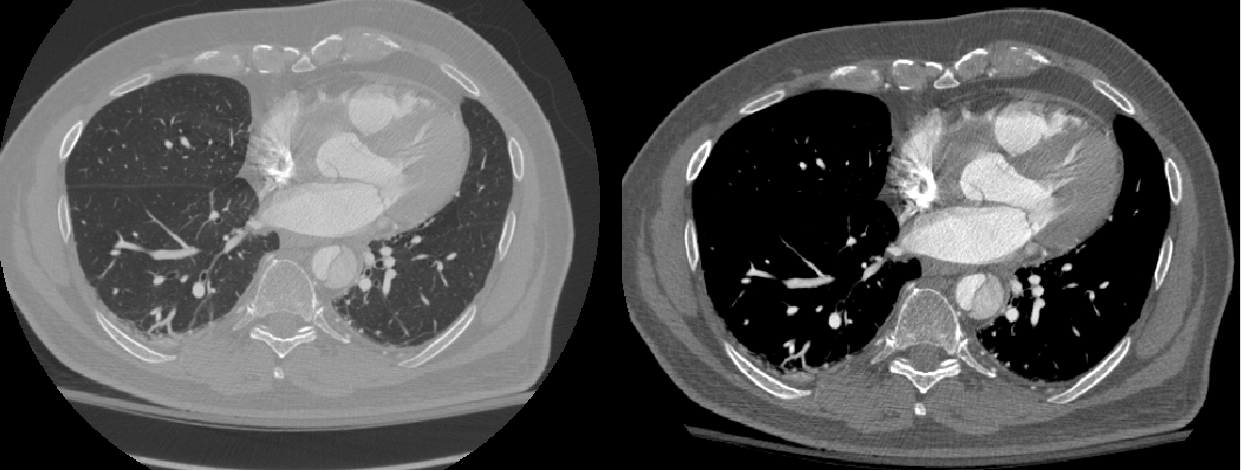
\includegraphics[width=\linewidth]{images/windowing-example}
 \caption{A cardiac CTA in its full range (left) and windowed (right). \cite{radlAVTMulticenterAortic2022a}}
 \label{fig:windowing-example}
 \end{figure}

\subsubsection{Magnetic Resonance Imaging (MRI)}

Much like CT, MRI produces voxel-based images that visualize the insides of an object. The process of obtaining an MRI image can be separated into several steps: 

\begin{enumerate}
	\item The machine applies a strong magnetic field to the subject. This causes protons in the body to align in the same direction --- parallel to the z-axis.
	\item Next, the machine emits a brief radio frequency pulse, perturbing the aligned protons and causing them to deviate from their uniform alignment.
	\item After the pulse is turned off, the protons gradually return back to alignment. As they realign, the movement of their positive charge induces an electric current in a coil inside the MRI machine. In contrast to CT, which gauges the attenuation of X-rays, MRI measures this induced current.
\end{enumerate}

The time to reach the equilibrium state depends on the specific tissue type, so the measured current allows the differentiation of tissues in the image. The equilibrium state is achieved through two independent processes: T1 and T2. T1 measures the time it takes the protons to reach equilibrium longitudinal alignment, while T2 measures the time to regain its equilibrium transverse alignment. Different tissues return to their equilibrium states at varying rates for T1 and T2, enabling two different types of MRI images: T1- or T2-weighted. For example, water exhibits a long T1 time, while fat has a shorter one. This means that in T1-weighted images, fat appears brighter than water, while the opposite is true in T2-weighted images. This can be seen in \figref{fig:t1-t2-example}.

\begin{figure}[h]
 \centering
 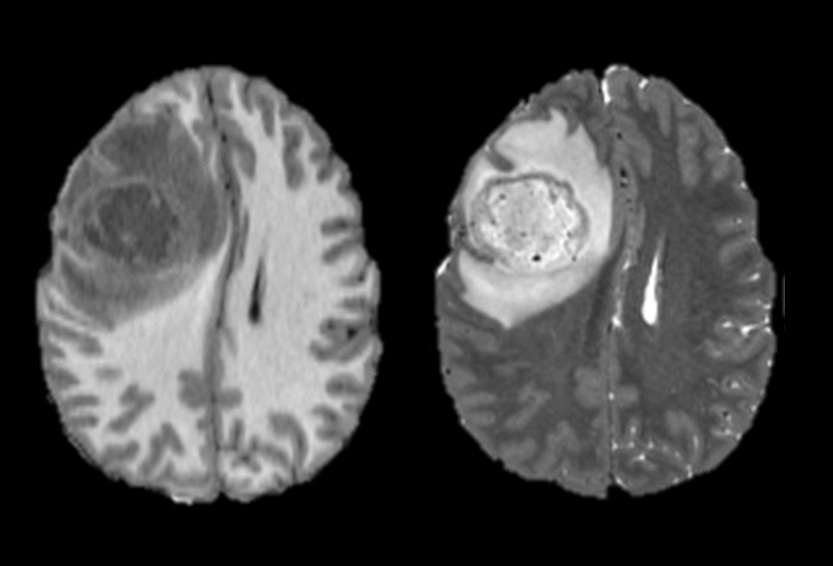
\includegraphics[width=0.65\linewidth]{images/mri-t1-t2-example}
 \caption{An example T1-weighted MRI (left) and a T2-weighted MRI (right) showing a diffuse glioma. \cite{calabreseUniversityCaliforniaSan2022}}
 \label{fig:t1-t2-example}
 \end{figure}
 
 The relative differences in T1 and T2 images make each more suitable for imaging specific tissues. For instance, T1-weighted images allow for identifying fatty tissue or detecting liver lesions, while T2-weighted images are more effective for identifying white matter lesions and edemas.
  
 The voxels in an MRI, much like a CT, are generally rectangular solids and can be different in width, height, and depth. The image resolution is determined by several factors, including the scanner's field of view, the MRI machine itself, and specific imaging parameters. Generally, increasing resolution leads to higher levels of noise and a longer acquisition time. Consequently, an optimal balance between resolution, noise, and scan time must be found, tailored to the tissue being imaged and the specific diagnostic objective.
 
 MRI has several advantages over CT. For one, MRI usually offers superior contrast, especially when imaging soft tissues. This has established MRI as the gold standard for a large number of diagnostic procedures. Much like with CT scans, MRI contrast can be further enhanced using contrast agents. Furthermore, as MRI uses magnetic fields instead of ionizing radiation, it poses no radiation-induced risks to patients.
 
However, MRI has its own set of limitations. MRI scans typically take longer than CT scans, which can be uncomfortable for patients, particularly those who are claustrophobic or have mental and cognitive disabilities. MRI is contraindicated for individuals with certain non-removable magnetic objects, like coronary pacemakers and specific implants. A notable drawback is the lack of standardization in MRI values across different scans and machines. Contrary to CT scans, an MRI voxel's intensity isn't consistent across different scans and can only be reliably interpreted in relation to adjacent tissue in the same scan.

\subsection{2D Modalities}

3D modalities, while offering a detailed view of a subject, often entail time-consuming and infeasible procedures in common clinical use. 2D modalities such as X-ray and diagnostic ultrasound are often quicker and more readily available. This ease and speed of 2D modalities contribute to the large amount of publicly available datasets in 2D modalities compared to 3D ones. For example, analyzing X-ray images is one of the most active fields in computerized medical image analysis research \cite{nguyen2020vindrcxr, irvinCheXpertLargeChest2019}.

\subsubsection{X-ray imaging}

X-ray imaging, also known as radiography, can be thought of as the 2D equivalent of a CT as it also relies on ionizing radiation. To obtain an image, X-rays are emitted on one side of the subject and captured on the opposite side. The intensity of the pixels corresponds to the attenuation of the emitted radiation. Denser materials appear with a higher intensity on the resulting image due to their high attenuation.

When capturing an X-ray image, an expert manually positions the generator. The relative positioning of this generator and the subject directly influences the image's magnification and field of view. If the subject is closer to the detector than the generator, it will appear magnified on the resulting image. Such magnification makes the scale on an X-ray image non-standard and precludes the possibility of making objective length and area measurements.

The expert also determines various parameters that ultimately change the quality and quantity of the X-ray beams. The quality measures the ability of an X-ray to penetrate tissue and is proportional to the X-ray energy level. Quantity, on the other hand, measures the number of photons constituting the beam. A high beam quality is advantageous for imaging denser tissues, like bones, or traversing larger volumes. However, high-quality beams reduce the contrast in soft tissues. Owing to the variability introduced by these parameters, X-ray image intensities lack the uniform standardization found in CT scans. Consequently, there's no standardized unit for gauging X-ray intensity across images.

\subsubsection{Dermatological images (clinical and dermatoscopic)}

The application of deep learning models to dermatology, especially skin lesion analysis, has gained significant momentum. This is driven in part by organizations such as the International Skin Imaging Collaboration (ISIC) which curates large dermatological datasets \cite{rotembergPatientcentricDatasetImages2021}. These datasets consist of two primary types of dermatological images: dermatoscopic and clinical. Clinical images are regular photographs of skin lesions, while dermatoscopic images are captured with a device called a digital epiluminescence dermatoscope. A dermatoscope consists of a camera attached to a magnifying lens with a built-in light source. It allows capturing detailed and magnified images of a skin lesion while filtering out skin reflections.

The primary application of deep learning in dermatological images is for classification, e.g. predicting whether a lesion is benign or not or detecting the type of skin disease. However, by precisely outlining the boundary of a skin lesion, segmentation techniques can yield more consistent and objective descriptors of the lesion, aiding classification algorithms \cite{rotembergPatientcentricDatasetImages2021}.

\subsubsection{Microscopy}

In biomedicine, one of the predominant uses of computer vision is in segmenting, analyzing, and quantifying microscopic images \cite{khanAutoCellSegRobustAutomatic2018}. This covers a broad array of tasks in digital pathology, from identifying cancerous cells and segmenting nuclei to quantifying white blood cell counts.

Publicly available microscopic images of cells are abundant due to how frequently they are captured and that they don't contain any personally identifiable information. However, the large size of these images can present a challenge. Often spanning multiple megapixels, they exceed the capacity of current deep-learning models and machines. Consequently, to make them more manageable, these images are typically divided into smaller patches, downscaled, or processed using a coarse-to-fine approach \cite{jhaInstanceSegmentationWhole2021a}.

As can be seen, both 2D and 3D biomedical images are exceedingly diverse in their appearance, use, technical details, and format. Yet, many segmentation techniques prove versatile enough to be applied across different modalities. In the next section, we will provide a general outline of how image segmentation works, highlighting commonly used methods.

\section{Image Segmentation: From Images to Segmentation Maps}

Image segmentation is the process of categorizing each pixel (or voxel) of an image into one of several predefined classes. Consider a 3-class segmentation scenario for CT images, with classes being liver, liver tumor, and background. Each of these classes is assigned a distinct numeric identifier, termed the \textbf{class label}. For illustration, the labels could be `0', `1', and `2' for the background, liver, and tumor respectively. The segmentation process outputs an image identical in dimensions to the original but with each pixel's value corresponding to the class label of that position in the original image. As an example, pixels corresponding to the liver will all have the value `1'. This resulting image is called a \textbf{segmentation map} since it, like a map, delineates important regions on the original image. 

In medical image segmentation, it's common to extract only a single tissue type against the backdrop, a technique known as \textbf{binary segmentation}. Additionally, multi-class segmentation challenges can be decomposed into multiple binary segmentation tasks, with each class having its individual class-vs-background segmentation map. Therefore, one can frame any segmentation problem as a set of binary segmentation problems.

Mathematically, given a set of $K$ classes, and an input $d$-dimensional image of $N$ channels $I(A)$, $I \in \mathbb{R}^{N}$, $A \in \mathbb{N}^d$ where A is the location of each voxel, the segmentation map $M : \mathbb{N}^d \rightarrow \mathbb{R}^K$ maps each pixel location to a vector of class probabilities:

\begin{equation}
M(A) = (\;\prg{C_1}{I(A)},\; \prg{C_2}{I(A)},\; \cdots\!,\;  \prg{C_{K}}{I(A)}\;),
\end{equation}

where $\operatorname{Pr} (C_i \!\mid\! I(A))$ is the probability that the voxel $I(A)$ contains an object of class $C_i$. Expressed this way, the segmentation map is a $K$-channel image of the same size as $I(A)$. Each channel of the image corresponds to a probability map of finding an object of a given class at a given voxel location. 

In binary segmentation, where $K=2$, the classes can be denoted as $C_1$ for the background and $C_2$ for the target object. Given this, for all voxel locations $A$, the relation $\prg{C_2}{I(A)} = 1 - \prg{C_1}{I(A)}$ holds true. Therefore $M(A)$ simplifies to a scalar value $M(A) = \prg{C_2}{I(A)}$. This representation is very common in medical image segmentation problems such as segmenting organs, cell nuclei, and skin lesions, among others.

Often, the next step in the process is to binarize the segmentation map $M(A)$. Voxels corresponding to the target object are set to `1', while the background is marked as `0'. In such cases, $M(A)$ is frequently termed a \textbf{segmentation mask}. In computer vision, ``mask'' refers to a binary image $M_{01}(A) \in \{0, 1\}$ that hides (masks) regions in another image, resulting in a masked image $I_m(A) = I(A) M_{01}(A)$. Within the context of deep learning-based image segmentation, the terms ``segmentation map'' and ``segmentation mask'' are often used interchangeably.

Having laid the foundation for the mathematical framework of image segmentation, we can now transition to exploring specific segmentation techniques. The next section presents an overview of common segmentation methods, from traditional ones based on heuristics to complex model-based approaches prevalent today.

\subsection{Traditional Image Processing Methods}

Despite the popularity of deep learning, traditional techniques, rooted in fundamental image characteristics, still play a vital role in modern medical image segmentation. Traditional techniques are often used as methods for pre-processing and data augmentation, as well as refining deep learning model outputs. As we will show later in the dissertation, traditional methods can increase the robustness and data efficiency of deep learning-based segmentation models.

Rather than relying on data-intensive training phases, these techniques often operate deterministically, using explicit algorithms that manipulate image characteristics. They directly use image properties such as intensity and texture, combined with heuristic strategies that draw from empirical observations and domain knowledge. Heuristics are best-practice rules derived from previous samples and experiences. For instance, the longest component in the bone intensity range of an X-ray image is usually the femur. These methods provide a clear, interpretable pathway to segmentation.

However, traditional methods are usually developed with a very specific application in mind and are hard to translate to other tasks and domains without significant changes. They are also sensitive to parameter selection and properties of the image such as intensity level. Helpfully, since they don't use a learning component their limitations can be known ahead of time. Their validity can also be confirmed using fewer samples than is the case for learning-based methods.

\subsubsection{Image Thresholding}

Thresholding is a fundamental technique that isolates regions in an image based on a specified range of intensities. In essence, it removes or retains portions of the image where the intensity either falls outside or within a given threshold.

To illustrate the use of thresholding, consider an example of segmenting adipose tissue on a CT scan. As mentioned earlier in this chapter, voxel intensities on CT scans quantify a tissue's X-ray radiation attenuation as measured in Hounsfield units. Typically, fatty tissue lies between -250 HU and -30 HU. Thresholding the entire scan to this range segments fatty tissue from all other tissues on the scan with no need for additional complex models. For preprocessing, Hounsfield unit thresholding is an efficient way to discard irrelevant voxels, allowing the rest of the segmentation process to focus on fewer voxels.

Thresholding can be also used to greatly simplify a model's task using domain knowledge. Take, for instance, the segmentation of epicardial fat, which refers to the fat in proximity to the heart wall. Epicardial fat is sparsely distributed in a complex shape inside the pericardium. Yet, the pericardium itself has a smooth, elliptical shape and is comparatively easy to segment. By first segmenting the pericardium and subsequently thresholding the pericardium region to the fatty tissue range, we can find epicardial fat without having to segment its complex shape directly \cite{bencevicRecentProgressEpicardial2022}.

\subsubsection{Region Growing Techniques}

Region growing is a voxel-based image segmentation method \citep{regionGrowing}. Beginning from a designated seed voxel, the method assesses neighboring pixels in successive steps. If these pixels meet a specified criterion, often related to pixel values or textures, they are integrated into the region. This process continues until all image pixels are assessed. Despite being a straightforward method, region growing is very sensitive to the selected seed point and may struggle with nuanced transitions between regions. This process is shown in \figref{fig:region-growing}.

\begin{figure}[h!]
 \centering
 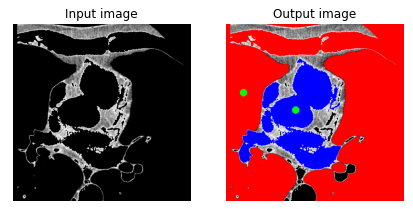
\includegraphics[width=0.7\linewidth]{images/region_growing.png}
 \caption{A demonstration of region growing for delineating the internal and external areas of the pericardium on a CT slice, set to the adipose tissue intensity range. The left image is the original input, and the right image depicts the segmented outcome with the heart exterior in red and the interior in blue. The green dots represent the manually chosen seed points initiating the region-growing technique. \cite{bencevicRecentProgressEpicardial2022}}
 \label{fig:region-growing}
 \end{figure}


\subsubsection{Active Contours or Snakes}

Active contours, often termed ``snakes'', are segmentation methods that employ dynamic curves to outline image parts \citep{Kass1988}. The process involves tightening a preliminary curve around an object iteratively until it conforms to the object's shape. The adaptation is guided by an energy function that evaluates the curve's smoothness and proximity to edges. A practical depiction of active contours is displayed in \figref{fig:active-contour}.

 \begin{figure}[h!]
 \centering
 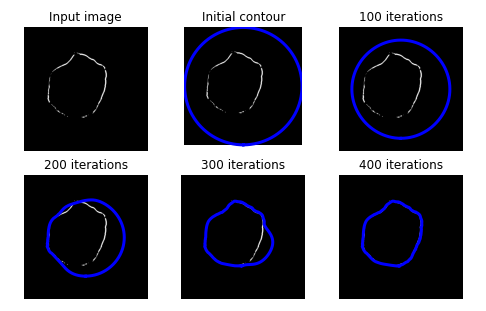
\includegraphics[width=0.65\linewidth]{images/active_contour.png}
 \caption{A demonstration of employing active contours to complete the absent segments of the pericardium line, displayed in white. The contour, illustrated in blue, starts as a complete circle surrounding the image. With every iteration, the contour adapts more closely to the image's shape. \cite{bencevicRecentProgressEpicardial2022}}
 \label{fig:active-contour}
 \end{figure}

\subsubsection{Atlas-Based Segmentation}

Atlas-based methods, differing from contour-based ones, leverage the spatial relationships among identified structures in an image \citep{Rohlfing2005}. First, a template image is selected and an expert creates an atlas (a segmentation map) by manually segmenting and labeling structures in the template image. Due to anatomical variations, multiple representative images are often merged to produce a template image. The atlas can then be employed to segment new images using a registration algorithm. Image registration is an optimization problem where one image, called the moving image, is deformed to best align with a target image according to some scoring function. The scoring function usually uses the distance between heuristic-based landmarks in the target and moving images to determine how well the two images align. In atlas-based segmentation, a new moving image is deformed to be aligned with the template image that was used to construct the atlas. The atlas can then be used as a segmentation map for the moving image, as it is now aligned with the atlas. The atlas-based registration process is illustrated in \figref{fig:registration}.

\begin{figure}[h!]
 \centering
 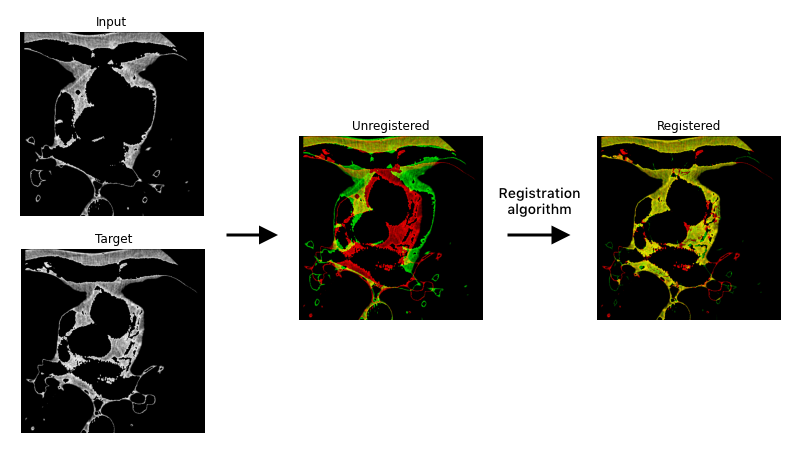
\includegraphics[width=0.7\linewidth]{images/registration.png}
 \caption{A schematic representation of the registration procedure. Initially, input and target images are chosen. Throughout the registration phase, the input image (shown in green) undergoes deformation to align with the fixed target image (shown in red). \cite{bencevicRecentProgressEpicardial2022}}
 \label{fig:registration}
 \end{figure}

A disadvantage of this approach is that the process can lead to a complete failure to segment the image if the target and moving images are too dissimilar. Therefore, atlas-based segmentation has fallen out of favor due to the emergence of deep learning-based methods. However, recently there has been significant progress in image registration and atlas-based segmentation using deep learning-based techniques \cite{sinclairAtlasISTNJointSegmentation2022a}. These approaches offer good potential for merging traditional and newer approaches will be discussed later in the chapter.

\subsection{Machine Learning}

While deep learning generally falls within the machine learning umbrella term, in this dissertation the term ``machine learning'' will be used to refer to techniques that are not based on deep neural networks. This encompasses methods such as support vector machines, random forests, and other statistical learning techniques that rely on manually engineered image features.

In this context, image segmentation can be viewed as a voxel-wise classification problem expressed as:

\begin{equation}
H(x; \theta) = (\;\operatorname{Pr}(C_0\!\mid\!x),\; \operatorname{Pr}(C_1\!\mid\!x),\; \cdots,\; \operatorname{Pr}(C_{K-1}\!\mid\!x)\;),
\end{equation}

where $H$ is a classification function parameterized by $\theta$, which maps an input vector $x$ of voxel-level features to the probability that the voxel contains the class $C_i$. The features are manually constructed based on domain knowledge and represent each pixel and its surrounding region. Commonly, these include the pixel's intensity, mean intensity of the area, image moments, and other information deemed relevant for the classification. The classifier is trained to minimize a predefined loss function by feeding each pixel's features to the classifier and comparing the output to the ground truth output. This is presented visually in \figref{fig:machine-learning}.

\begin{figure}[h!]
 \centering
 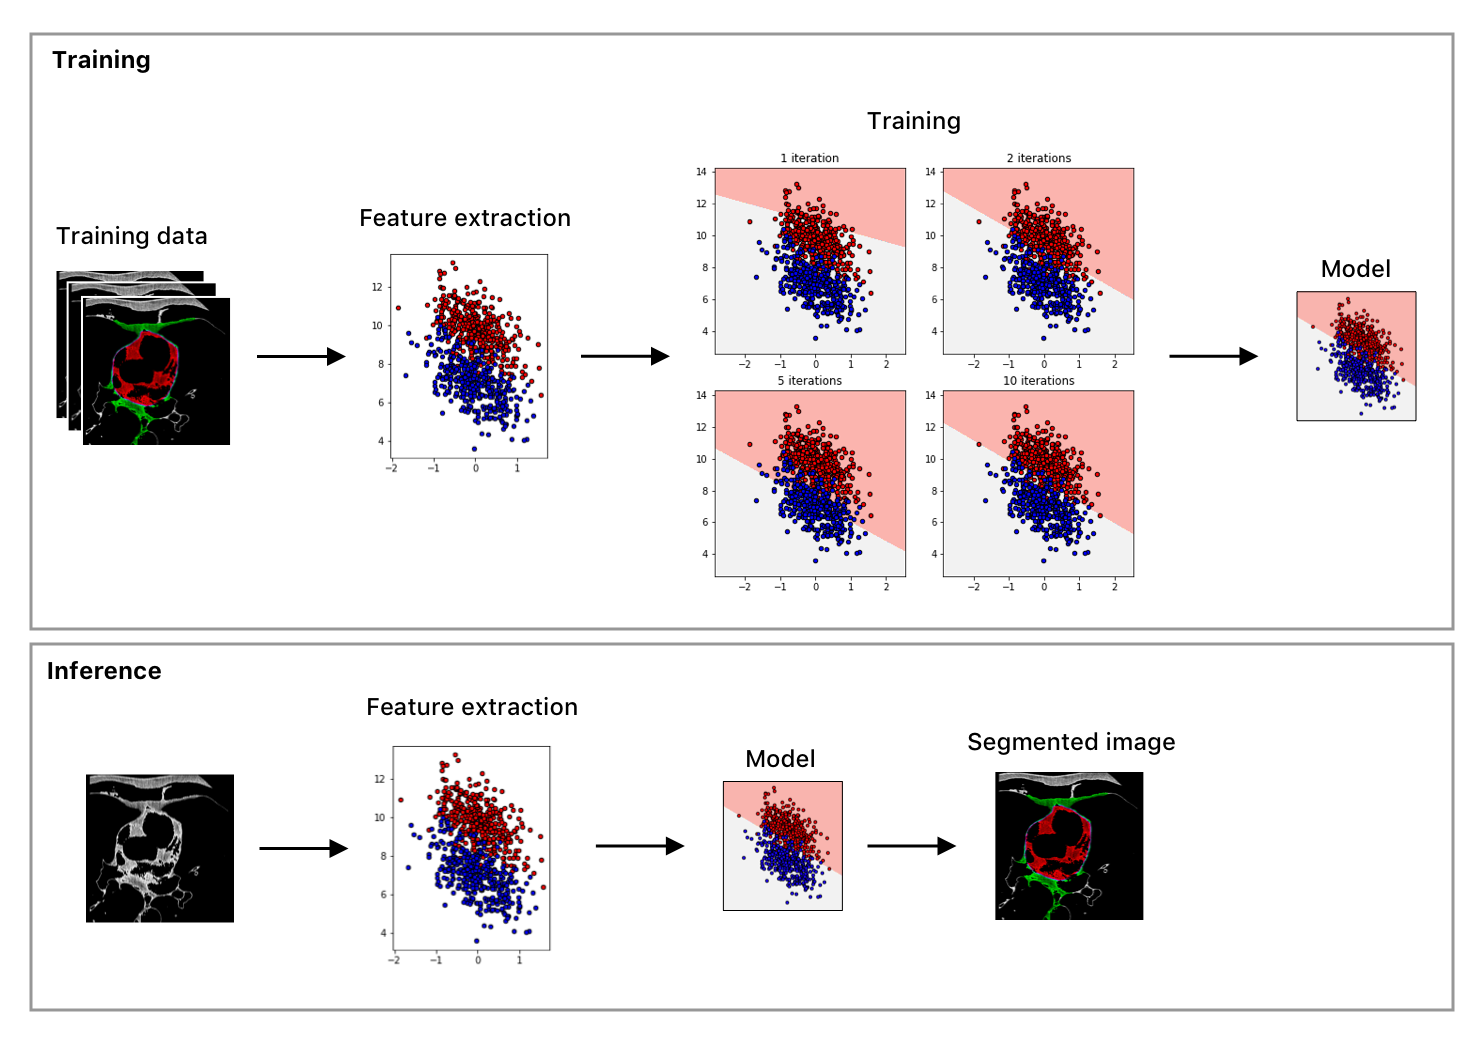
\includegraphics[width=\linewidth]{images/machine_learning.png}
 \caption{A schematic of a supervised linear classifier in a machine learning workflow. The upper section illustrates the training phase. Here, features are color-coded according to their known class from training data, depicted in red and blue. The parameters of the decision boundary, which demarcates the zones of the two classes (highlighted in light red and grey), are determined during training. The lower part of the diagram depicts the inference stage. In this phase, features are extracted from new images, and the trained model is employed to classify each pixel in the image. \cite{bencevicRecentProgressEpicardial2022}}
 \label{fig:machine-learning}
 \end{figure}

Another common approach is to divide the image into smaller patches and then employ a machine learning classifier to categorize each patch into one of the predefined $K$ classes. The classifications are then fused together to form a segmentation map. Both patch- and voxel-based machine learning approaches can be more data efficient than deep learning-based approaches \cite{bencevicRecentProgressEpicardial2022}, but they often lack the ability to model complex features and dependencies. 

It is clear that these traditional techniques have inspired and paved the way for more complex deep learning methods --- while still playing a vital role as parts of segmentation pipelines today. In the next section, we will provide an overview of how deep learning builds on traditional machine learning to achieve more powerful models that can segment very complex regions.

\pagebreak

\section{Deep Learning-Based Segmentation Methods}

Machine learning encompasses a broad range of techniques for building statistical models, which includes deep learning --- a subset of machine learning that focuses on using artificial neural networks. Artificial neural networks consist of simple nodes called \textbf{neurons}. Each neuron is a non-linear function of the sum of its inputs. This non-linear function is called the \textbf{activation function}. The neurons are all arranged in a graph where the outputs of one set of neurons are connected to the input of another set of neurons. Each connection has an associated \textbf{weight} and \textbf{bias} parameter. The value on the connection is multiplied by the weight and the bias is added before it's fed into the subsequent neuron. The exact configuration of the graph, including the number of neurons and how they are connected, is determined by hand and is referred to as the \textbf{neural network architecture}. Typically neurons are arranged into \textbf{layers}, where neurons of one layer connect only to the next layer. Current deep-learning networks usually have between ten and 100 layers. A typical neural network architecture can be seen in \figref{fig:nn-typical}.

\begin{figure}[h!]
 \centering
 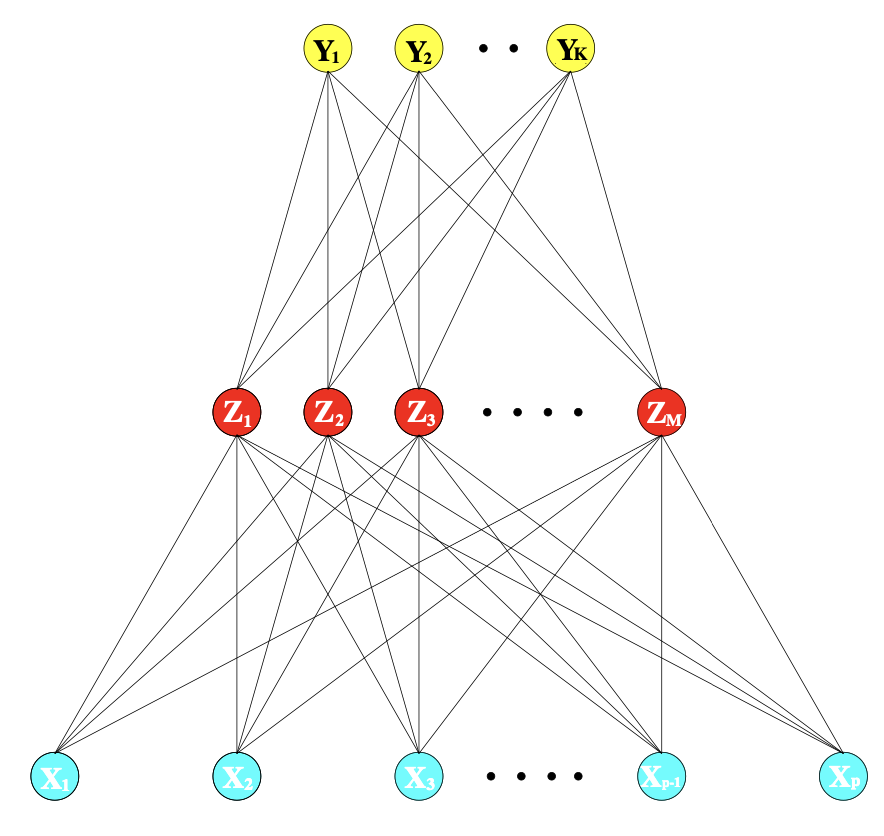
\includegraphics[width=0.5\linewidth]{images/nn-typical}
 \caption{A small neural network with three layers, wherein each layer is connected to every neuron in the next layer. \cite{hastieElementsStatisticalLearning2009}}
 \label{fig:nn-typical}
 \end{figure}

Mathematically, a neuron is a function that maps some input vector to a scalar value. First, the dot product between the input vector $x = [x_0\; x_1\; \cdots\; x_{n - 1}]$ and the weights column vector $w$ is calculated and added with the bias vector $b$:

\begin{equation}
z(x;w, b) =
\begin{bmatrix}
x_0 & x_1 & \cdots & x_{n - 1}
\end{bmatrix}
\begin{bmatrix}
w_0\\
w_1\\
\cdots\\
w_{n-1}
\end{bmatrix}
+
\begin{bmatrix}
b_0 & b_1 & \cdots & b_{n - 1}
\end{bmatrix}
\end{equation}

Then, all of the inputs are summed and the neuron output is produced using the activation function $af$:

\begin{equation}
f(x;w,b) = af\left(\sum_{i=0}^{n - 1} z(x;w,b)_i\right).
\end{equation}

The parameters $b$ and $w$ associated with each neuron can be consolidated into a large matrix, denoted as $\theta$. This matrix is called the \textbf{parameters of the network}. Current deep learning networks usually have multiple millions of parameters.

One example of an activation function is the rectified linear unit (ReLU) function:

\begin{equation}
ReLU(x) = 
    \begin{cases}
        x, & \text{if } x > 0,\\
        0, & \text{otherwise.}\\
    \end{cases}
\end{equation}

ReLU can be seen as a simple thresholding function that sets all negative values to zero. Despite its simplicity, ReLU is one of the most prevalent activation functions in neural networks.

\subsection{Neural Network Training, Validation and Testing}

Initially, the parameters of a neural network are often initialized with random values. These values are then fine-tuned during a procedure called \textbf{training}, which iteratively adjusts the parameters to minimize a \textbf{loss function}. The loss function measures how well the network is performing its task by comparing its output to known correct values. For example, in image segmentation, the loss function would measure the similarity between the network's segmentation map and a hand-labeled counterpart. Through a process called \textbf{backpropagation}, each parameter is updated in the direction that will decrease the loss. This is repeated multiple times for each image in a \textbf{training dataset}.

However, there's a caveat. The training dataset, much like any statistical data, is a sampling of the ``real world'' data from some unknown distribution. Depending on the size and quality of the dataset, it is possible that the training dataset does not represent the true distribution of the data. Moreover, the network can learn to produce correct solutions for each training image individually instead of learning general patterns in the data. This is called \textbf{overfitting} --- the model excels on the training data but fails on unseen data. To detect and mitigate this, two additional datasets are introduced: the \textbf{validation} and \textbf{test} datasets.

The \textbf{validation dataset} serves a critical role during model development. After training, the model is assessed using this dataset to inform decisions about its architecture, preprocessing, and other facets. During the development cycle, the network is constantly modified and re-evaluated on the validation dataset. Since adjustments to the model are based on its performance on the validation dataset, there's a risk of inadvertently tailoring the model to the specific distribution of the validation data. To counteract this potential bias, a \textbf{test dataset} (often termed a hold-out dataset) is used. This dataset is reserved exclusively for a final evaluation, offering the least biased estimate of the model's real-world performance.

The training, validation, and testing datasets are created before the model development process. Usually, they are sampled randomly from a larger dataset with ratios such as 80\%, 10\% and 10\% for the training, validation, and testing datasets, respectively. 

In the next chapter, we will further discuss overfitting in neural networks. For now, we will move on to describing neural network architectures in more detail.

\subsection{Encoders and Decoders}

Machine and deep learning-based segmentation methods can be conceptualized as a two-stage process. The first stage, termed the \textbf{encoder} stage, is a function $En : \mathbb{R}^{D \times C} \rightarrow \mathbb{R}^{n \times m \times d}$. In other words, a $D$-dimensional image with $C$ channels is mapped to a feature vector. This vector has an arbitrary size and depth determined by the network architecture. The encoder effectively compresses the image by distilling salient information into a smaller representation, the feature vector. In deep learning parlance sometimes this is referred to as the \textbf{backbone} of the network.

The output of the encoder then goes to the second stage called the \textbf{decoder} or the \textbf{head}. The decoder is a function $De : \mathbb{R}^{n \times m \times d} \rightarrow \mathbb{R}^{D \times K}$ that maps a given feature vector into a segmentation map. 

Given an image $I(A)$, the segmentation process can then be written as:

\begin{equation}
M(A) = (En(\theta_{En}) \circ De(\theta_{De}))(I(A)),
\end{equation}

where $En$ and $De$ are functions parameterized by a $\theta_{En}$ and $\theta_{De}$, respectively. In conventional machine learning, $En$ is not a trainable function. Instead, $\theta_{En}$ consists of hand-selected parameters to extract pre-selected features from the image. The value of $\theta_{De}$, on the other hand, is determined by minimizing a loss function. In deep learning, both $\theta_{En}$ and $\theta_{De}$ are determined by minimizing a loss function.

Thus, the difference between traditional machine learning and deep learning is in the encoder stage. Deep learning utilizes neural networks to define features, whereas traditional machine learning uses handcrafted functions.

The separation of segmentation models into encoder and decoder stages is a crucial aspect of current research in deep learning. This separation allows for independent improvement of both stages and an easy combination of different encoders and decoders. For instance, a classification and segmentation network could use the same encoder architecture. While the classifier would utilize a simpler decoder to map input features to a class probability vector, the segmentation model would employ a more complex decoder to produce a segmentation map. However, both models would use the exact same encoder. In fact, there are models such as Mask R-CNN \cite{heMaskRCNN2017b} that use two parallel decoders, one for segmentation and another for object detection, both connected to the same encoder. Throughout the rest of this thesis, when describing neural network architectures, we will describe them in terms of their encoder and decoder and how the two are connected.

\subsection{Convolutional Neural Networks}

Convolutional neural networks have profoundly impacted computer vision, establishing deep learning as the prevailing approach for complex computer vision tasks. The foundational element of a \ac{cnn} is its convolutional layer, which uses a convolution-like operation in place of the conventional neurons mentioned earlier in this chapter.

\subsubsection{Convolution}

\begin{figure}[h!]
 \centering
 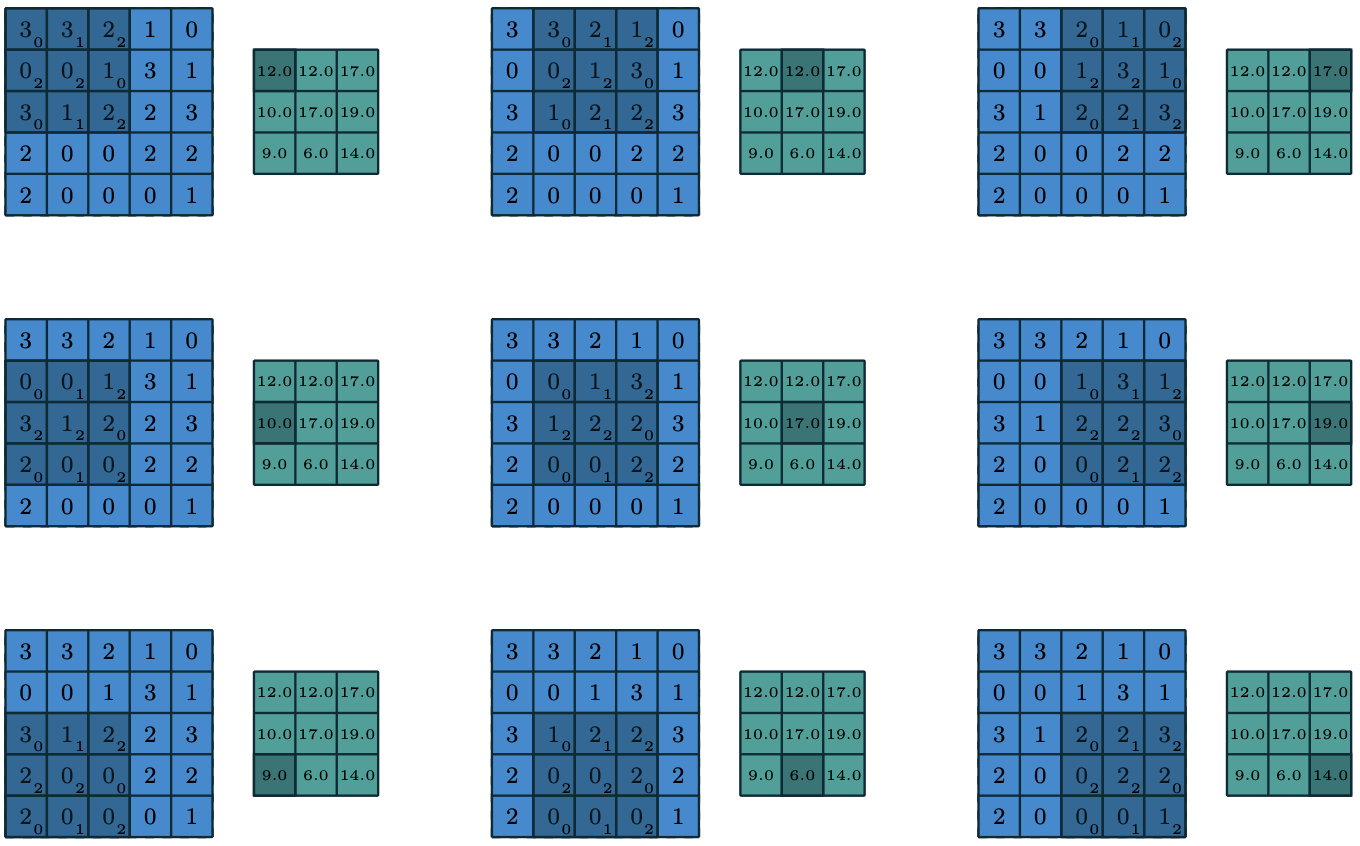
\includegraphics[width=\linewidth]{images/convolution-explainer.png}
 \caption{A visual depiction of a convolution procedure step-by-step. In each step, the kernel slides over the image (shown in blue). The overlapping elements between the kernel and the image are multiplied and then summed to produce a value in the resultant image (shown in green). \cite{dumoulinGuideConvolutionArithmetic2018}}
 \label{fig:convolution-explanation}
 \end{figure}

Generally, convolution is a mathematical operation between two functions. In the context of this thesis, however, we will focus on discrete 2D convolution between two square images, as that is most relevant for image segmentation. Convolution is denoted as $I(A) \star k(B)$ where $I(A)$ is an image $I(A) \in \mathbb{R}^{W \times H}$ and $k(B)$ is a matrix $k(B) \in \mathbb{R}^{w \times h}$ indexed by locations $B \in \mathbb{N}^2$ for called the \textbf{convolutional kernel}. At position $A = (a_x, a_y)$, the convolution operation is defined as:

\begin{equation}
(I \star k)(a_x, a_y) = \sum_{j=-\infty}^{\infty} \sum_{i=-\infty}^{\infty} I[i, j] k[a_x - i, a_y - j].
\end{equation}
 
Explained differently, the resulting image is produced by sliding the kernel over the input image pixel by pixel. At each pixel location, values where the kernel and the image overlap are multiplied, and all of the products are summed together to form the corresponding pixel's value in the output image. This is shown visually in \figref{fig:convolution-explanation}.

While mathematically a simple operation, convolution is exceedingly powerful and can produce almost endless transformations of an image. It's most commonly used for filtering --- a convolution can elegantly find patterns in the image and increase their intensity in the image. One such example is the convolution with a kernel called the Prewitt operator:

\begin{equation}
I_y(A) = I(A) \star \begin{bmatrix}
-1 & 0 & 1\\
-1 & 0 & 1\\
-1 & 0 & 1\\
\end{bmatrix}
\end{equation}

When convolved with this kernel, the resulting image has high-intensity pixels in regions where vertical edges are present, and low intensity everywhere else. This can be seen in \figref{fig:prewitt-example}.

\begin{figure}[h!]
 \centering
 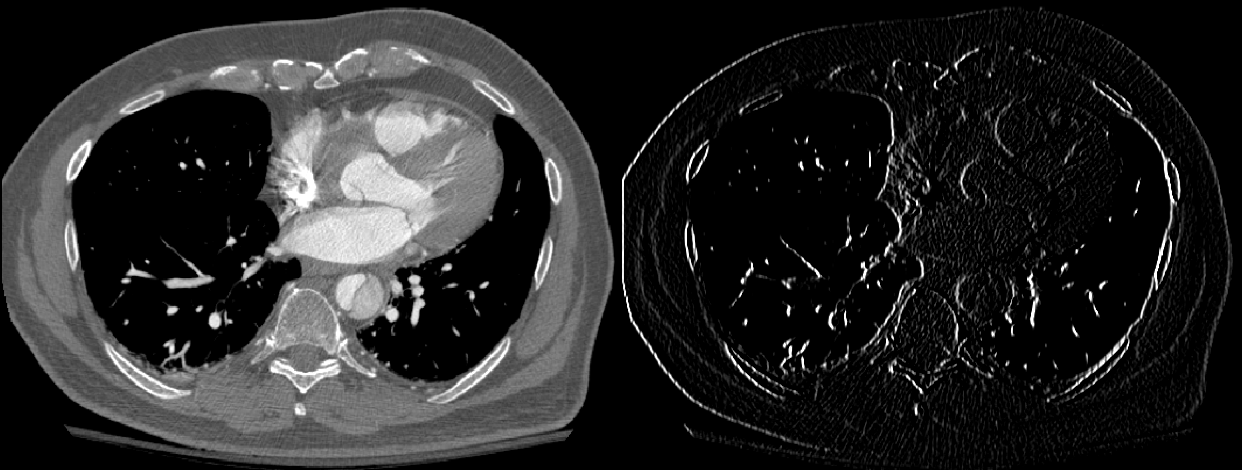
\includegraphics[width=\linewidth]{images/prewitt-example.png}
 \caption{An example of an input image (left) convolved with the Prewitt operator (right). Note that vertical edges are accentuated in the convolution result.}
 \label{fig:prewitt-example}
 \end{figure}

Vertical edges necessarily have to have a large jump in values going from left to right or right to left. Otherwise, there would be no perceptible edge. This kernel takes advantage of that fact to accentuate parts of the image where there is such a jump. It does this by replacing each pixel with the difference between the pixels on its left and its right.

This process happens as follows. For each pixel of the input image, the kernel is placed such that it is centered on that pixel. This means that the values of the pixel as well as its neighbors above and below are all multiplied by zero. The neighbors on the left are multiplied by -1, and the ones on the right are multiplied by 1. Summed together, the result represents the sum of the values on the right of the pixel, minus the sum of the values on the left.

To illustrate this, let us consider $1 \times 3$ region of the image where no vertical edges are present:

\[
\begin{bmatrix}
128 & 130 & 136\\
\end{bmatrix}
\star
\begin{bmatrix}
-1 & 0 & 1\\
-1 & 0 & 1\\
-1 & 0 & 1\\
\end{bmatrix}
=
\sum_{i,j}
\begin{bmatrix}
-1 \times 0 + 0 \times 128 + 1 \times 130\\ 
-1 \times 128 + 0 \times 130 + 1 \times 136\\
-1 \times 130 + 0 \times 136 + 1 \times 0\\
\end{bmatrix}
= 8
\]

This section of the image does not contain a vertical edge, so the convolution result is a relatively low value. In a standard image with values in $[0, 255)$, 8 would appear almost completely black.

However, consider some section of the image where a vertical edge is indeed present:

\[
\begin{bmatrix}
63 & 66 & 132\\
\end{bmatrix}
\star
\begin{bmatrix}
-1 & 0 & 1\\
-1 & 0 & 1\\
-1 & 0 & 1\\
\end{bmatrix}
=
\sum_{i,j}
\begin{bmatrix}
-1 \times 0 + 0 \times 64 + 1 \times 66\\ 
-1 \times 64 + 0 \times 66 + 1 \times 132\\
-1 \times 66 + 0 \times 132 + 1 \times 0\\
\end{bmatrix}
= 68
\]

The value is now much larger due to the difference between the left and right sides of the image. This example demonstrates how a relatively simple kernel can capture complex features of an image.

Beyond edge detection, there are many commonly used convolution kernels to perform tasks such as blurring, sharpening, or denoising images. A \ac{cnn} can leverage the power of the convolution by stringing together sequences of intricate kernels to match complex patterns in the image.

\subsubsection{Convolutional Layers}

A \ac{cnn} operates by passing an image through a sequence of convolutions. The output from one convolution serves as the input for the next. Interspersed between these convolutions are non-linear transformations of the outputs. This layered approach enables the network to successively find more and more intricate features by combining simpler ones. For instance, combining edges into corners, corners into shapes, and ultimately detecting objects from shapes. The addition of non-linearity drastically increases the complexity of features the network is able to detect and combine.

More technically, in a \ac{cnn}, convolutional layers are connected to one another in a similar fashion to neurons in a regular neural network. Each layer performs a set number of convolutions, denoted by $n$. The results are stored in an $n$-channeled \textbf{feature map}. Each channel corresponds to a convolution with a distinct kernel. Hence, a convolutional layer contains $n$ unique kernels. The values of the kernels are the parameters of the layer, optimized during training to minimize a loss function like weights and biases of standard neurons. Finally, a convolutional layer also applies a non-linear activation function to the resulting feature map.

It's worth noting that the operation within a convolutional layer differs from a standard 2D discrete convolution. Here, both the kernel and the input are three-dimensional and have the same depth, but the kernel is usually much smaller in width and height. Since the kernel has the same width as the input, during the operation the kernel only slides along the width and height dimensions. The output of each sliding window step is still a single scalar since all overlapping elements in the sliding window volume are multiplied and summed together. This means that the output of the whole operation is a two-dimensional image. This is visualized in \figref{fig:cnn-conv-explained}.

\begin{figure}[h!]
 \centering
 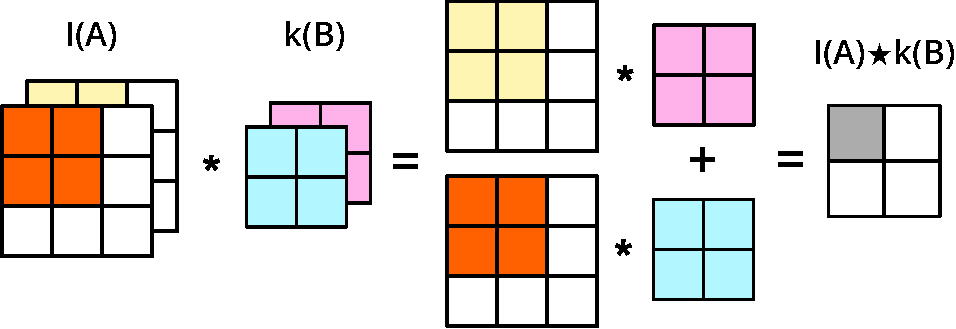
\includegraphics[width=0.8\linewidth]{images/cnn-operation-explained}
 \caption{A view of one step of a single convolution operation inside a \ac{cnn} layer. The layer performs multiple convolutions, each with a different kernel that has an equal number of channels as the input image. In each step, the whole kernel slides over the width and height of the image, and the overlapping channels are multiplied together and summed to produce a single output value. The output of the convolution is one channel of a $n$-channel image where $n$ is the number of different kernels in the layer.}
 \label{fig:cnn-conv-explained}
 \end{figure}
 
\subsubsection{Pooling Layers}

Most \ac{cnn}-based encoders follow a pattern of gradually reducing the width and height of the feature maps while increasing their depth. Depth is increased by giving each successive convolutional layer more kernels. Since each channel represents the result of a convolution with a specific kernel, having more kernels directly increases the output depth. To reduce the width and height, \textbf{pooling layers} are employed. These layers downsample the image, often by averaging pixel values within a defined neighborhood. This downsampling serves dual purposes in a CNN. Firstly, it compresses the image by gradually removing spatial information and retaining relevant semantic information. Secondly, the network is gradually able to build up large complex features by combining small general features. Such an architecture is shown in \figref{fig:cnn-encoder-achitecture}.

\begin{figure}[h]
 \centering
 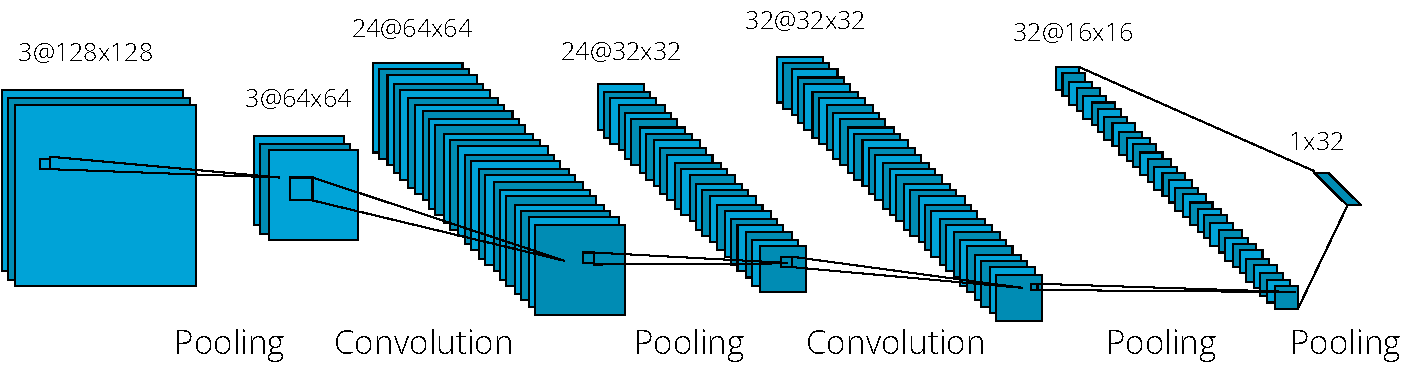
\includegraphics[width=\linewidth]{images/cnn_encoder_example.pdf}
 \caption{A typical architecture of a \ac{cnn} encoder. The encoder consists of consecutive convolutional and pooling layers that gradually increase the feature map depth and decrease its width and height. The result is a map of features that tells the decoder what features are on the image but does not provide much spatial information about the location of those features. \cite{lecunGradientbasedLearningApplied1998}}
 \label{fig:cnn-encoder-achitecture}
 \end{figure}

To illustrate this, consider a contrived example of a \ac{cnn} encoder trained to detect grapes on a vine. The first few layers might focus on simple operations such as edge detection, requiring a large amount of spatial information. The next layer could use the edge information to detect circles. This layer doesn't need as much spatial detail since the edges are already identified. A third layer might then combine the locations of the circles to detect a cluster of grapes. By this stage, the spatial information is even less important, with the overall arrangement of circles being the primary focus.

A convolutional decoder essentially reverses the encoder process. Instead of adding channels, a convolutional decoder successively removes channels up to and upsamples the image. By the end, the output matches the input image's width and height, and the number of output channels equals the number of classes.

One way in which upsampling is implemented in a convolutional decoder is with a \textbf{transposed convolutional layer}. These layers are very common in segmentation neural networks and allow for dynamic, learned upsampling of the image. Regular convolutions cannot increase the image dimension width and height. To overcome this, a transposed convolution produces an output matrix for each step of the sliding window process, instead of just a scalar value. For instance, a transposed convolution with a $2 \times 2$ kernel produces 4 new values for each pixel in the input image. This is done by performing scalar multiplication of the whole kernel and the pixel it is sliding over during each sliding window step. All of the sliding window results are joined as a grid to form a final, larger, image.

To better understand this, consider an example of upscaling a $2 \times 2$ 2D input image $m$ with a $2 \times 2$ kernel $k$. The transposed convolution can be calculated as follows:

\begin{align*}
m \star^T k = & 
\begin{bmatrix}
m_{11}k_{11} & m_{11}k_{12} & 0\\
m_{11}k_{21} & m_{11}k_{22} & 0\\
0 & 0 & 0\\
\end{bmatrix}
+
\begin{bmatrix}
0 & m_{12}k_{11} & m_{12}k_{12}\\
0 & m_{12}k_{21} & m_{12}k_{22}\\
0 & 0 & 0\\
\end{bmatrix}
+\\
&
\begin{bmatrix}
0 & 0 & 0\\
m_{21}k_{11} & m_{21}k_{12} & 0\\
m_{21}k_{21} & m_{21}k_{22} & 0\\
\end{bmatrix}
+
\begin{bmatrix}
0 & 0 & 0\\
0 & m_{22}k_{11} & m_{22}k_{12}\\
0 & m_{22}k_{21} & m_{22}k_{22}\\
\end{bmatrix}
\end{align*}

This method can be similarly applied to images and kernels of any size. While transposed convolution is often referred to as \textit{deconvolution}, in this thesis, we will avoid using the term to prevent confusion with the meaning of deconvolution outside of the context of deep learning.

Segmentation models that use only convolutional and pooling layers are called \textbf{fully convolutional models} and are one of the most widely used types of models for medical image segmentation. In the following section, we will describe these and other commonly used CNN architectures in medical image segmentation.

\section{CNN Architectures for Medical Image Segmentation}

Deep learning's application in medical image segmentation has predominantly seen the use of convolutional neural networks. This field has witnessed a rapid evolution, giving rise to a diverse range of architectures. While some of these architectures were initially designed for general image classification and segmentation tasks, others have been specifically tailored to overcome challenges specific to medical imaging. In this section, we will highlight the most influential CNN architectures that have shaped medical image segmentation, presented in their chronological development.

\subsection{Fully Convolutional Network (FCN)}

The fully convolutional network (FCN), one of the more straightforward contemporary CNN architectures for image segmentation, was introduced in \cite{long2015fully}. As mentioned earlier, convolutional encoders gradually downsample the image while increasing the number of channels in the feature maps. There is then a need to reverse the process and decode the features into an image of equal width and height as the original input image. FCN achieves this using convolutional layers and upscaling.

In FCN, the output of the encoder is interpreted as a coarse heatmap of detected features. An output segmentation map needs to be constructed based on these features and have a number of channels equal to the number of classes. FCN does this by using a convolutional layer with $1 \times 1$ kernels --- one kernel for each class. The resulting convolutions combine the features depth-wise to form a class prediction for each location of the image. However, the resulting segmentation map has a very low spatial resolution. To be useful, it needs to be upsampled using transposed convolution to the original image resolution.

As noted earlier, the encoder's output feature map is only a rudimentary representation of spatial details. To inject additional spatial information into the final segmentation, FCN combines predictions from multiple encoder layers to form the final prediction. This is done by upsampling $1 \times 1$ convolution results from different encoder layers to a uniform size and summing them together. The composite prediction is then upsampled to the original image resolution. This process is shown in \figref{fig:fcn-arch}. 

\begin{figure}[h!]
 \centering
 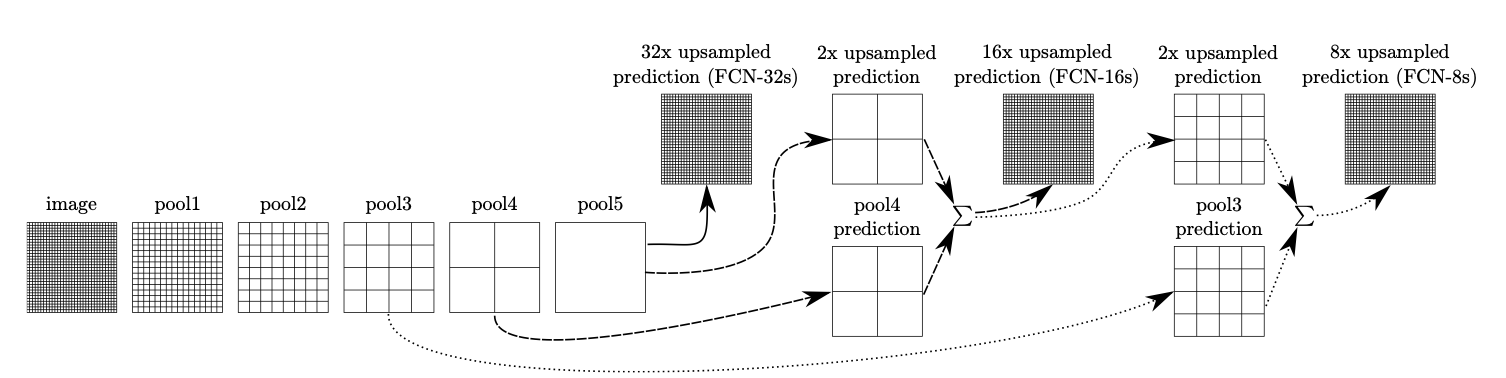
\includegraphics[width=\linewidth]{images/fcn-arch}
 \caption{A diagram of how FCN forms predictions based on the output of different encoder layers. Encoder layers are shown on the left and the grid represents the coarseness of the feature map. The maps are combined at three different levels to produce three predictions. Each prediction is compared with the ground truth during training, but for inference only the 8x upsampled prediction is used. \cite{long2015fully}}
 \label{fig:fcn-arch}
 \end{figure}
 
 \subsection{U-Net and Its Variants}

U-Net \cite{ronnebergerUNetConvolutionalNetworks2015d} is one of the most influential and commonly used architectures in medical image segmentation. Aside from being a standard baseline model, a well-tuned U-Net network with data preprocessing has reached state-of-the-art performance in various segmentation challenges across different domains and modalities \cite{isenseeNnUNetSelfconfiguringMethod2021}.

At its core, U-Net follows a straightforward architectural pattern, comprised of a fully convolutional encoder and decoder with only convolutional and pooling layers. The encoder and decoder have a symmetrical structure: the encoder gradually decreases the width and height of the feature maps while increasing the number of channels, while the decoder does the opposite using upsampling or transposed convolutions. While FCN uses only one $1 \times 1$ convolutional layer and upsampling to form a prediction, U-Net uses a sequence of several convolutional and upsampling layers to gradually build a segmentation map. This progressive structure allows U-Net to produce more detailed feature maps.

Earlier we that spatial information is important for the precise localization of the features. Like FCN, U-Net also uses the outputs of different encoder layers to maintain spatial information in the decoder but does so in a different way. In U-Net, the output of every encoder layer is added to the input of its corresponding decoder layer on the other side of the network. This gives each decoder layer concurrent access to information about which features are on the image and where they are located. U-Net's architecture can be seen in \figref{fig:unet-arch}.

\begin{figure}[h!]
 \centering
 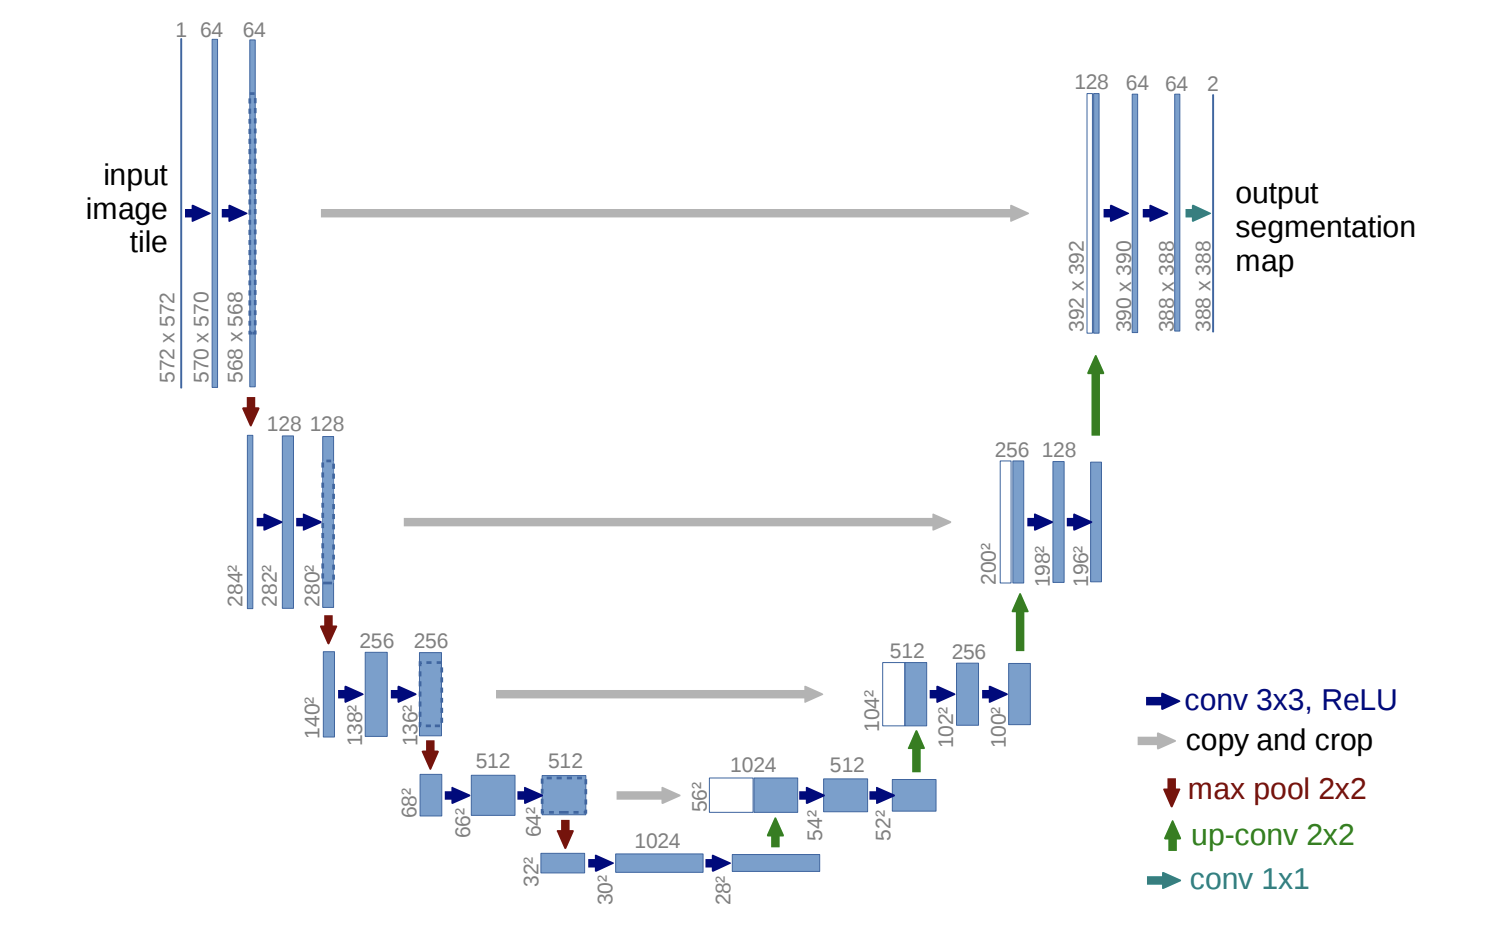
\includegraphics[width=0.8\linewidth]{images/unet-arch}
 \caption{A diagram of the U-Net model. The output of each layer of the encoder is concatenated to the input of its corresponding layer in the decoder. \cite{ronnebergerUNetConvolutionalNetworks2015d}}
 \label{fig:unet-arch}
 \end{figure}

Because of its symmetrical structure and skip connections, U-Net is often visualized in the shape of the letter U, giving it its name. U-Net is only one of a class of networks that are sometimes called U-shaped networks. Aside from being a state-of-the-art architecture for medical image segmentation, U-Net is also widely used as a component of influential deep learning models in other domains such as image generation \cite{rombach2021highresolution} and registration \cite{sinclairAtlasISTNJointSegmentation2022a}.

\subsubsection{nnU-Net}

U-Net is a powerful baseline model that can be carefully tuned using various heuristics and combined with beneficial data preprocessing to achieve state-of-the-art results, even when compared to much more complex models. However, tuning the parameters of the model and preprocessing is a laborious process that requires experise and empirical research. nnU-Net \cite{isenseeNnUNetSelfconfiguringMethod2021} aims to automate this tuning process by producing an optimal data pre- and postprocessing pipeline and a U-Net-based architecture for a given dataset. This is achieved through a set of heuristics, rules, and optimization techniques.

The nnU-Net framework begins by calculating key parameters of the data distribution, such as intensity distribution and median image size. These parameters feed into a set of predefined rules that determine the network's architecture and training strategy, including the number of layers, training parameters, and preprocessing approach.

Using the determined parameters, nnU-Net trains three models: one using 2D slices of the data, another using the entire 3D volume, and the third using a cropped 3D region of interest. During inference, outputs from these models are combined through preprocessing to form an ensemble prediction, enhancing the overall accuracy and robustness of the segmentation. This process is shown in \figref{fig:nnunet-arch}.

\begin{figure}[h!]
 \centering
 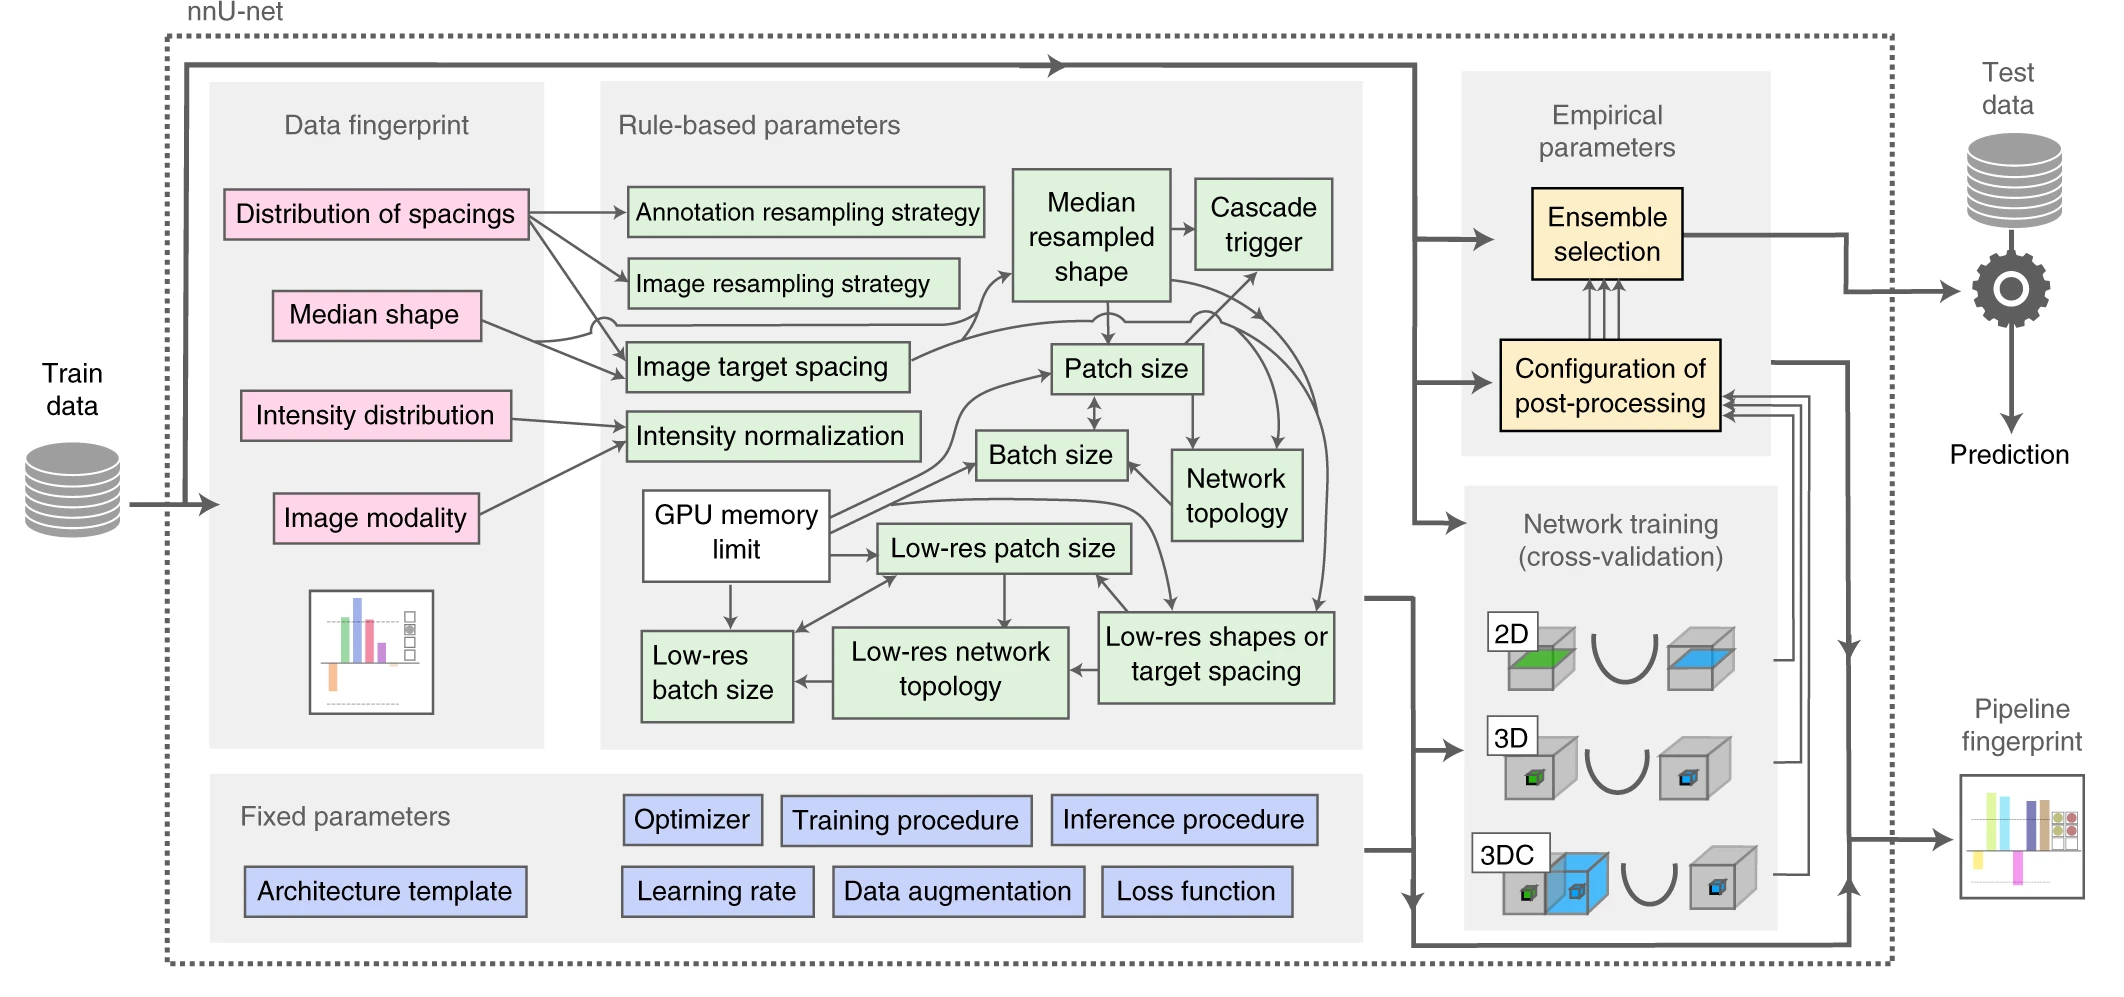
\includegraphics[width=\linewidth]{images/nnunet-arch}
 \caption{A diagram of the nnU-Net procedure of creating a training configuration. \cite{isenseeNnUNetSelfconfiguringMethod2021}}
 \label{fig:nnunet-arch}
 \end{figure}
 
 nnU-Net has demonstrated exceptional performance, establishing itself as a state-of-the-art solution in a variety of CT and MRI segmentation tasks. nnU-Net is a hugely important tool for both academia and industry, as it allows for creating well-tuned baseline models with very little manual intervention or technical expertise.
 
 Furthermore, nnU-Net exemplifies the critical role of preprocessing and parameter tuning in improving model performance, particularly when working with small datasets. This is the cornerstone of this thesis: improving data efficiency through preprocessing. The success of nnU-Net serves as a validation of this approach.
 
 \subsubsection{U-Net++}
 
In standard U-Net, skip connections link encoder layer outputs to decoder layer inputs through basic concatenation operations. This approach leaves room for more intricate integration of the decoder and encoder outputs. Additionally, U-Net only merges features at corresponding levels of the encoder and decoder. An enhancement to this could be to allow each decoder layer access to features from multiple encoder layers. U-Net++ \cite{zhou2019unetplusplus} takes advantage of these opportunities with a flexible architectural design.

In U-Net++, skip connections are reimagined as a network of convolutional layers. This setup connects each encoder layer to its respective decoder layer through multiple convolutional layers.  This enhances the information fed into the skip convolutional layers. Additionally, the outputs of these skip connections are further upscaled and fed into the subsequent decoder layers. This design results in a significantly more complex network architecture. Here, each decoder layer not only receives features from its direct encoder counterpart but also from all deeper encoder layers. This multifaceted connection system is visually represented in \figref{fig:unetpp-arch}.

 
 In U-Net++, skip connections are reimagined as a network of convolutional layers instead of simple concatenation. Moreover, outputs from each encoder layer (except the first) are upscaled and then supplied as additional inputs to the skip connections of the preceding layer. The outputs of the skip connections themselves are also upscaled and given to the next corresponding decoder layer. Thus, each decoder layer not only receives features from its direct encoder counterpart but also from all deeper encoder layers. This architecture is presented in \figref{fig:unetpp-arch}.
 
 \begin{figure}[h!]
 \centering
 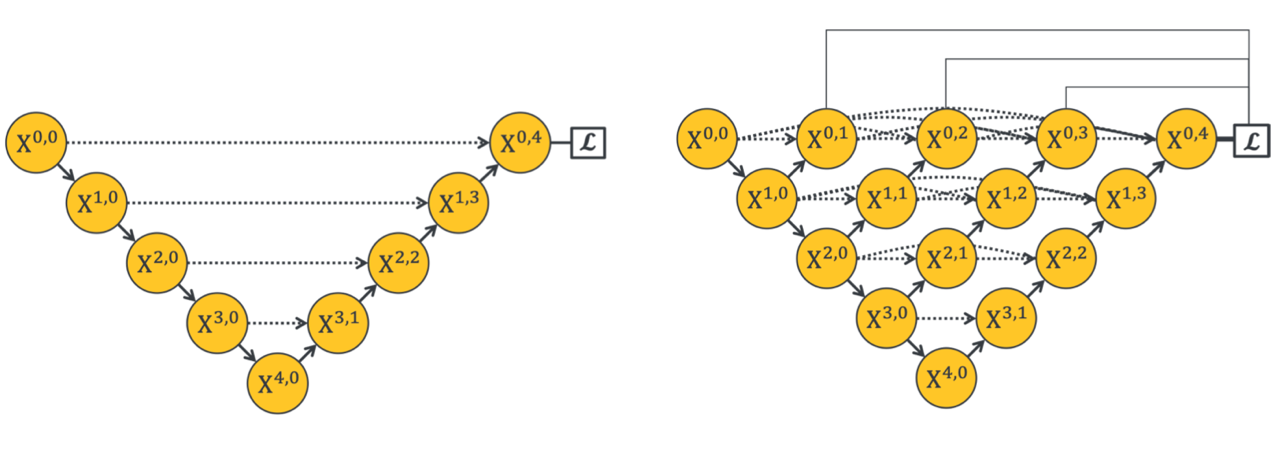
\includegraphics[width=\linewidth]{images/unetpp-arch}
 \caption{A comparison between U-Net (left) and U-Net++ (right). Each node in the graph represents a convolutional layer. The dashed arrows represent skip connections, while full arrows are downsampling or upsampling operations. \cite{zhou2019unetplusplus}}
 \label{fig:unetpp-arch}
 \end{figure}
  
There are several advantages to U-Net++ over U-Net. Each decoder layer has access to multi-scale features of the input image and thus can produce more accurate outputs. Conceptually, U-Net++ can be viewed as an ensemble of U-Nets with varying depths, which helps in faster convergence compared to a standard U-Net of similar depth. Further, instead of finding the optimal U-Net depth, due to the flexibility of neural networks, U-Net++ learns the optimal depth during training. This makes U-Net++ more flexible, requiring fewer design decisions. However, U-Net++ has a higher parameter count and does not necessarily enhance data efficiency. In some cases, its performance benefits can be matched or surpassed by a well-preprocessed and tuned U-Net \cite{isenseeNnUNetSelfconfiguringMethod2021}.

\subsection{Mask R-CNN}

Earlier in the chapter we mentioned that CNN-based segmentation networks generally consist of encoder and decoder stages. Segmentation architectures such as U-Net employ a decoder that progressively upsamples the feature maps to construct a segmentation map. This differs from how object detection decoders work.

Object detection aims to find the location of an object in an image. Instead of classifying each pixel as in segmentation, object detection typically outputs the coordinates of a bounding box surrounding the object. In technical terms, the output is not an image but rather a vector of four numbers for each object. As such, the decoders in object detection networks are usually much shallower and employ fully connected layers instead of convolutional layers.

Despite these differences, both object detection and segmentation networks share similar encoder designs. Mask R-CNN \cite{heMaskRCNN2017b} takes advantage of this to combine object detection and segmentation into a single network. In Mask R-CNN, a standard CNN encoder generates a feature map from an input image. This map is then given to two parallel decoders: one for segmentation and the other for object detection. The segmentation decoder, akin to those in standard segmentation networks, uses convolutional layers and upsampling to generate a segmentation map for each object. The detection decoder, in contrast, employs downsampling and fully connected layers to output the bounding box and class label of each object. The Mask R-CNN architecture can be seen in \figref{maskrcnn-arch}.

 \begin{figure}[h!]
 \centering
 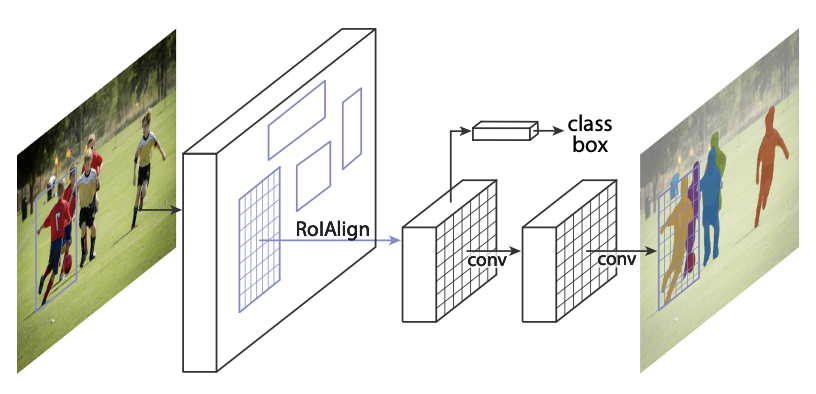
\includegraphics[width=0.6\linewidth]{images/maskrcnn-arch}
 \caption{A diagram of the Mask R-CNN architecture. Two parallel decoder branches are used to achieve segmentation and object detection simultaneously. \cite{heMaskRCNN2017b}}
 \label{fig:maskrcnn-arch}
 \end{figure}

Consequently, for every detected object, Mask R-CNN provides a bounding box, a class label, and a segmentation mask. The network is trained using a composite loss function, optimizing for segmentation, detection, and classification simultaneously.

The integration of these tasks in Mask R-CNN takes advantage of synergies between them. The information learned for classifying an object is relevant to its detection. Similarly, by using a bounding box the segmentation decoder can focus on the relevant portion of the image and be invariant to the scale of the object on the image. This joint learning approach enhances performance across all tasks compared to training separate networks for each. However, Mask R-CNN's complexity can pose challenges, particularly when trained on very small datasets, where simpler segmentation-focused architectures like U-Net might be more effective.

\subsection{Other Notable Segmentation CNNs}

A central challenge in CNN-based segmentation is balancing spatial information with feature complexity. As the network increases the feature map depth and decreases width and height, spatial information is erased but more complex features can be detected on the image. Effective segmentation requires both elements. While U-Net addresses this with skip connections, other architectures use different methods to integrate multi-scale features.

One approach involves pyramid pooling, as utilized in PSPNet \cite{zhao2017pspnet}. Initially, PSPNet uses a standard encode to create a feature map. This map is then rescaled to various sizes, and each rescaled map undergoes processing through a series of convolutional layers. The resulting outputs from these layers are resized to a uniform spatial dimension and concatenated. This combined feature map is then fed into a decoder to produce the final segmentation map.

Pyramid pooling is also employed by DeepLabV3 \cite{chen2017rethinking} albeit in a different way. Like in PSPNet, the encoder first creates a feature map. This feature map then goes through a series of parallel layers that each use an atrous convolution. In atrous convolution, the kernel is dilated by introducing gaps between its values. During each sliding window step, the gaps are ignored and the result is convolved regularly for non-empty kernel values. This technique enables covering a larger area of the image without increasing kernel parameters. Each parallel layer uses different gap sizes in the kernel, creating multi-scale features. These features are upscaled, merged, and further decoded into a segmentation map.

MA-Net \cite{manet} takes a different route by incorporating an attention mechanism for combining multi-scale features. Rather than directly concatenating in skip connections like U-Net, MA-Net introduces a multi-scale attention block. This block aims to capture the interdependencies of different features to focus on more salient ones before they are concatenated to the decoder layer input. Additionally, the final decoder layer is processed through a position-wise attention block to highlight significant features in specific image locations. MA-Net has shown performance improvements in liver tumor segmentation on CT images compared to U-Net and U-Net++.

\section{Fully Connected Transformers for Medical Image Segmentation}

So far most of this chapter dealt with CNNs. However, another class of networks --- transformers \cite{attnAllYouNeed} --- has recently gained traction and even surpassed the segmentation quality of CNNs for many tasks. The key to the transformer's impressive performance is the ability to support very deep neural networks. Empirical observations suggest that with enough data, network performance tends to increase with the depth of the network. Hence, transformers have become state-of-the-art in tasks where a large amount of data is available. Notably, current transformers used in natural language processing contain more than 100 layers and trillions of parameters, orders of magnitude more than CNN-based models.

Transformers first became broadly used in the field of natural language processing and achieved groundbreaking results in text generation, machine translation, and understanding natural language. Broadly, transformers employ a combination of regular (non-convolutional) fully connected layers and attention mechanisms, which are the key to their success. Attention allows a layer to learn the interdependencies between parts of its input or across different input values. In linguistic contexts, this leads to a more nuanced understanding of syntactic relationships, enabling the network to learn concepts such as the interplay between subjects and objects or the likelihood of certain adjectives preceding specific nouns.

\subsection{Attention}

For each element $x_i$ of an input sequence of length $n$, an attention mechanism aims to produce a vector $v_i = (v_{i1}, v_{i2}, \cdots, v_{in})$ where $v_{ij}$ measures how dependent $x_i$ is on $x_j$. In a natural language scenario, if we consider a sentence as our input sequence, this mechanism can be envisioned as going word by word, and for each word producing relevance scores for every other word in the sentence. For instance, in the sentence ``Susan has a brown dog that she loves.'', the word ``she'' should have a high relevance score for ``Susan'', and a low score for ``brown'' since it is not pertinent to encoding the meaning of ``she'' in this sentence.

Mathematically, attention can be expressed as a series of matrix multiplications. First, each input sequence element is transformed into a query vector. This transformation represents a learned encoding by the network, converting an input element into a lower-dimension vector. The query serves to identify the current input element in the sequence. Let $X$ be an input matrix where each row is a new element of the sequence. Let $W_Q$ be a matrix of weights learned by the network that encodes each element of the input sequences into a vector. The query matrix $Q$ can then be calculated as:

\begin{equation}
Q = W_Q X
\end{equation}

Where each row $Q_i$ represents the query for $X_i$. Remember that the goal of attention is to score the relevance between an input element $X_i$ and some other element $X_j$ of the same input sequence. Having encoded each element $X_i$ in the form of $Q_i$, we need to similarly encode each $X_j$ in a different matrix $K$ where $K_j$ is called the \textbf{key} for some input sequence element $X_j$. We can do so as:

\begin{equation}
K = W_K X,
\end{equation}

where $W_K$ is another weight matrix that the model optimizes during training. Given $K$ and $Q$, we can compute the relevance scores for every combination of input elements $x_i$ and $x_j$ as:

\begin{equation}
A = Q K^T,
\end{equation}

Here, $A_{ij}$ represents the relevance score between $x_j$ and $x_i$. It is important to note that this is only one of many ways the matrix $A$ can be calculated. In practice, $A$ is scaled to be in $[0, 1]$ or transformed in some other way.

Finally, to get the output $Z$ of the self-attention layer, we weigh each element of the original input sequence $X$ by the attention scores $A$:

\begin{equation}
Z = A V,
\end{equation}

$Z$ consists of $X$ elements weighted by how relevant they are to the encoding of the whole sequence. Visually, this process for one element of the input sequence can be seen in \figref{fig:attention-explainer}.

 \begin{figure}[h!]
 \centering
 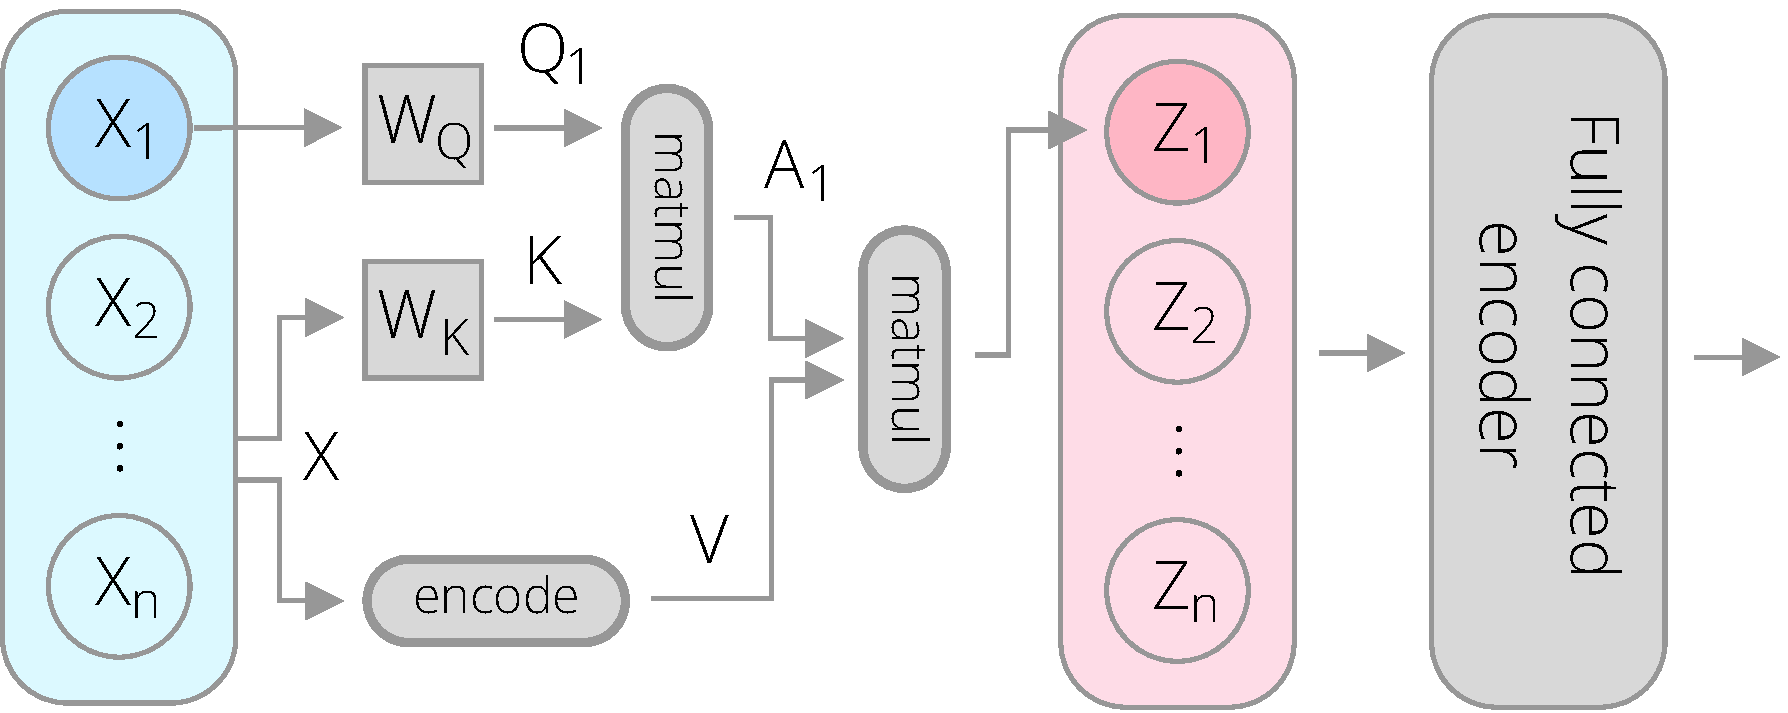
\includegraphics[width=0.8\linewidth]{images/attention-explainer}
 \caption{A visualization of a single encoder layer in a transformer network. This shows the encoding process for one element of the input sequence.}
 \label{fig:attention-explainer}
 \end{figure}
 
 Encoder and decoder layers in a transformer include an attention layer followed by a fully connected layer. In the encoder, the attention layers are generally \textit{self-attention}, where both the key and the query come from the input sequence. In contrast, the decoder layers employ both self-attention and \textbf{encoder-decoder attention}. In the latter, the keys and values come from the encoded features of the last layer of the encoder. Finally, each attention layer performs $Z$ calculation multiple times using different $W$ and $K$ weights, and the weighted values are concatenated together. This design enables the network to simultaneously learn and apply various types of attention within each individual layer.
 
 \subsection{Positional Encoding}
 
The position of each word in a sentence carries important information. The sentence ``The yellow notebook is on top of the red notebook.'' has a different meaning than ``The red notebook is on top of the yellow notebook.'', even though both sentences contain the same words. To capture this in transformers, the position of each input element is encoded and included as part of the input.
 
Each input sequence element index is mapped to a matrix via a function $f : \mathbb{Z}^{+} \rightarrow \mathbb{R}^d$ where $d$ is the dimensionality of the layer's input. Mapped that way, the positional encoding can simply be concatenated to the layer's input with no additional changes in the network. While it's possible for this encoding function to be represented as neural network layers and learned during training, a common approach is to use a predefined, fixed function. For instance, in cite{attnAllYouNeed}, given an element index $pos$, the $i$-th element of the positional encoding is calculated as:

\begin{equation}
PE(pos, i) = \begin{cases}
	\sin(pos/1000^{2i/d}), & \text{$i$ is even}\\
	\cos(pos/1000^{2i/d}), & \text{$i$ is odd.}\\
\end{cases}
\end{equation}

The choice of positional encoding functions is guided by their numerical characteristics, ensuring they are efficiently processed by the neural network.
  
 \subsection{Adapting Transformers to Image Segmentation}
 
 Convolutional Neural Networks (CNNs) have traditionally dominated image processing due to their efficiency in handling large inputs. Consider a $128 \times 128$ pixel image which, when flattened into a row vector, results in 16,384 elements. In a fully connected network, where each input element connects to every output element, this translates into $16,384^2$ parameters for just one layer. Even if the image were to be heavily downscaled and ignore the loss of information this would create, managing such a network on current GPUs is infeasible.
 
 Transformers that use fully connected layers face a challenge when applied to image data due to this very issue. The key solution, as utilized in the Vision Transformer (ViT) \cite{dosovitskiy2021an}, is treating an image as a sequence of small patches, allowing the image to be processed similarly to text.
 
 ViT, primarily designed for image classification, begins by partitioning each image into uniform square patches (e.g. $32 \times 32$ pixels). The patches, ordered starting from the top-left of the image, form an input sequence $X$. Each patch is then flattened to a row vector and given to a fully connected layer to encode it as a $d$-dimensional vector. Then, a $d$-dimensional positional encoding is added to the encoding as a function of the patch index. The resultant matrix serves as the input for the encoder, which operates identically to a standard transformer network. This architecture can be seen visually in \figref{fig:vit-arch}.
 
  \begin{figure}[h!]
 \centering
 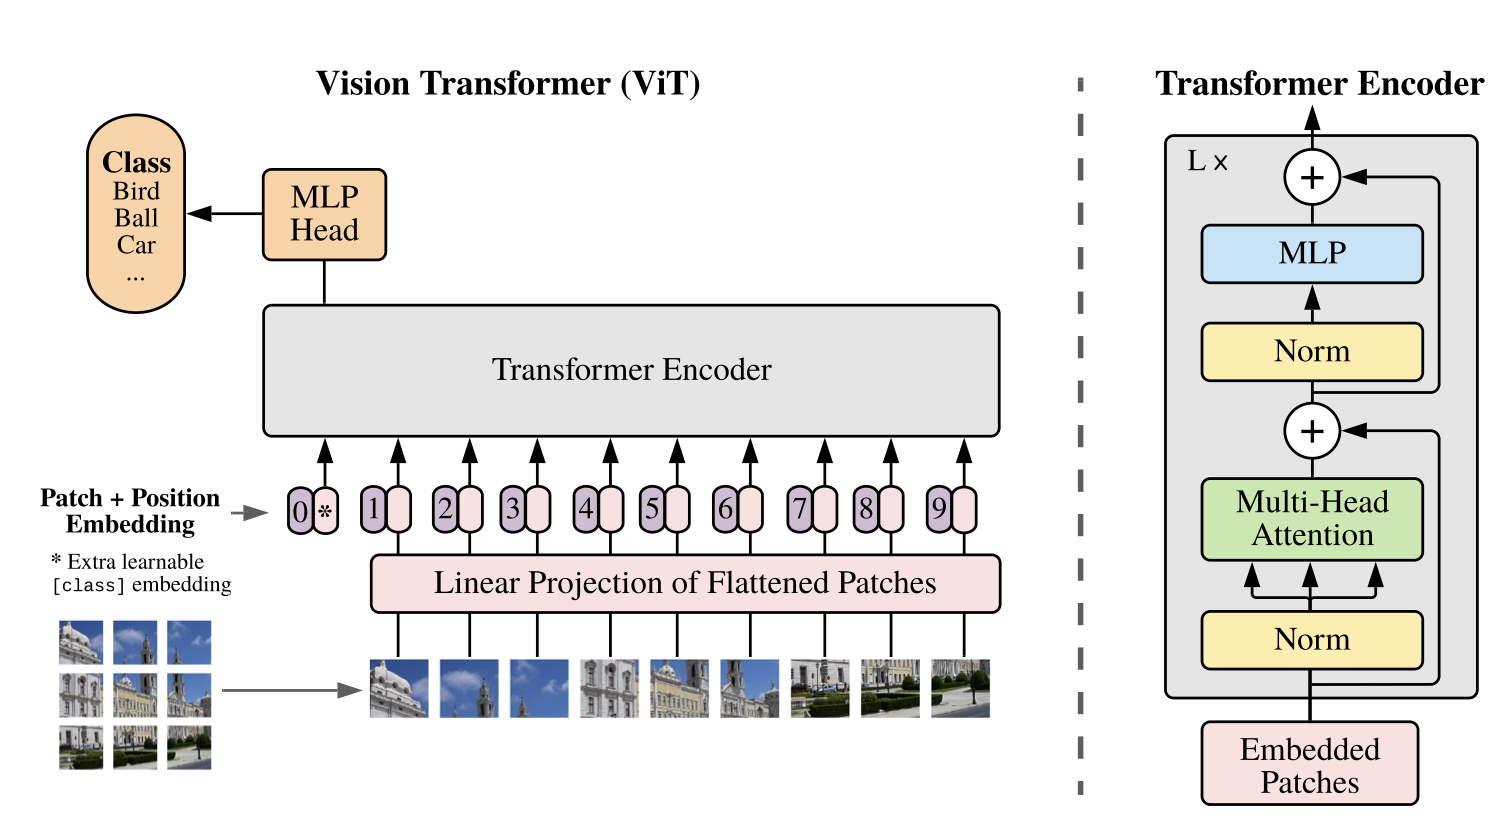
\includegraphics[width=\linewidth]{images/vit-arch}
 \caption{The ViT architecture for image classification. \cite{dosovitskiy2021an}}
 \label{fig:vit-arch}
 \end{figure}
 
 While ViT originally used a classification decoder, it is possible to combine the ViT encoder with a segmentation decoder to obtain a segmentation map. There are several ways this has been achieved. For instance, the Segmentation Transformer (SETR) \cite{SETR} introduces two distinct CNN-based segmentation decoders connected to a ViT encoder. The first variant follows a conventional convolutional decoder design, where the encoder's output goes through a series of upsampling and convolutional layers, producing a segmentation map in the original image resolution. The second decoder variant is similar to the way FCN works --- outputs from various encoder layers are resized to a uniform resolution, merged, and then decoded into a segmentation map.

 Later transformer-based segmentation networks modified the ViT encoder as well. For instance, the authors of the Swin Transformer \cite{liu2021Swin} argue that neural networks for computer vision need to be built with translation and scale invariance in mind. Swin Transformer starts with small patches, similar to ViT, but in each successive encoder layer neighboring patches are merged. Rather than computing self-attention within individual patches, Swin uses non-overlapping windows of multiple patches to perform self-attention. This ensures that Swin’s computational demand increases linearly with image size, a significant improvement over ViT’s exponential growth. A key aspect of Swin is that each successive layer shifts the window by half of the window size. This allows self-attention between two different windows and more global information about the image. Finally, Swin's encoder output is fed into a DeepLab-like decoder to produce the segmentation map.
 
 Transformers have demonstrated exceptional performance in image segmentation, particularly in large datasets and benchmarks with upwards of 20,000 natural images \cite{liu2021Swin, SETR, chen2022vitadapter}. However, their advantage is less pronounced in smaller datasets. This aligns with observations from \cite{attnAllYouNeed} --- convolutional layers have properties that are naturally a good fit for extracting information out of images. Transformers need to compensate for their lack of convolutions by using more layers. However, as we will see in the next chapter, there is a relationship between the number of parameters of a network and the number of samples required to train that network.



\printbibliography[heading=subbibintoc]
\end{refsection}

\begin{refsection}
% Kapitel 3

\chapter{Data Efficiency in Neural Network-Based Image Segmentation}
\label{chap:data-efficiency}

Above all, the accuracy of neural networks is governed by three factors: problem complexity, model complexity, and sample size. Each of these factors contributes to accuracy in different ways and they have complex interdependent relationships. Grasping the concept of data efficiency necessitates an understanding of these three aspects. In this chapter, we will elucidate how the three factors impact model error by examining neural networks as function approximators.

Consider a machine learning scenario where we estimate the 10-year risk of heart disease based on age. Here, some underlying function maps age to heart disease risk. However, there is no way to know what this function is. Our only recourse is to collect a set of data points and try to approximate the underlying function. Our goal is to iteratively search for a function that minimizes some criterion that measures the discrepancy between the function and our collected data points.

One can construct an infinite number of functions that fit a set of data points equally well under a selected criterion. Therefore, to derive a single solution, we have to choose a finite class of functions to evaluate. One of the simplest classes of functions we could use is lines --- leading to a simple linear regression. A line is defined by two parameters, its slope $\theta_1$ and intersect $\theta_0$:

\begin{equation}
	f(x) = \theta_1 x + \theta_0.
\end{equation}

In this equation, $f(x)$ represents our regression model. The objective is to determine the optimal value of $\theta = \{ \theta_1, \theta_2 \}$ that most accurately represents the collected data pairs $(x_i, y_i)$. This can be achieved by minimizing the mean squared distance between the line and each data point:

\begin{equation}
	\min_{\theta} \sum_{i=1}^N (y_i - f(x_i))^2.
\end{equation}

We will conduct a simulated experiment. We will construct an underlying function as a cosine function, with each point sampled with additive Gaussian noise:

\begin{equation}
	y(x) = -(\cos(0.01 \pi x) - 1) \cdot 0.4 + Z, Z \sim \mathcal{N}(0, 0.1).
\end{equation}

We will generate several $(x_i, y_i)$ pairs and apply the previously discussed linear model and criterion to fit a line through these points. In real-world conditions, the underlying function and the nature of the measurement noise remain unknown. However, for this simulation, knowing these details is useful to demonstrate the divergence between the fitted function and the underlying one. Figure \ref{fig:t1-t2-example} illustrates the fitted line using varying numbers of data points.

\begin{figure}[h!]
 \hfill
 \subfloat{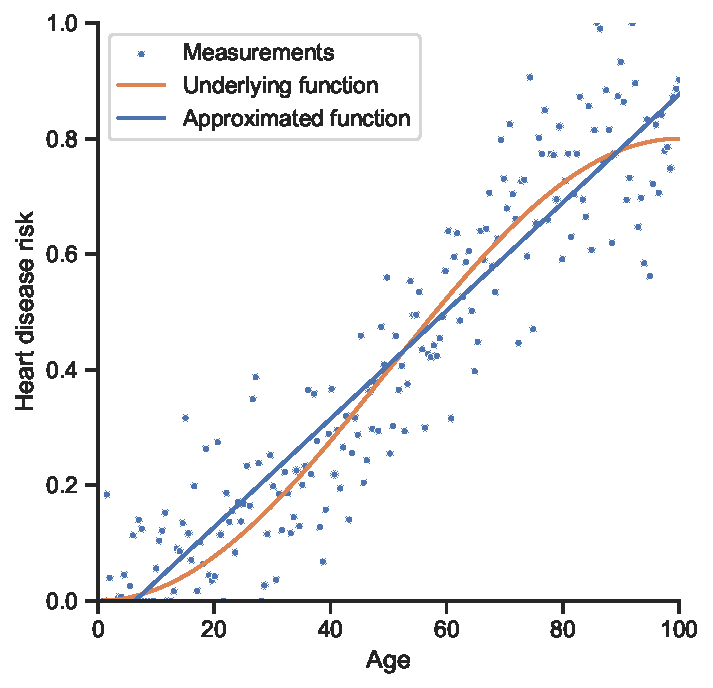
\includegraphics[width=0.5\linewidth]{images/3/heart_disease_risk}}
 \hfill
 \subfloat{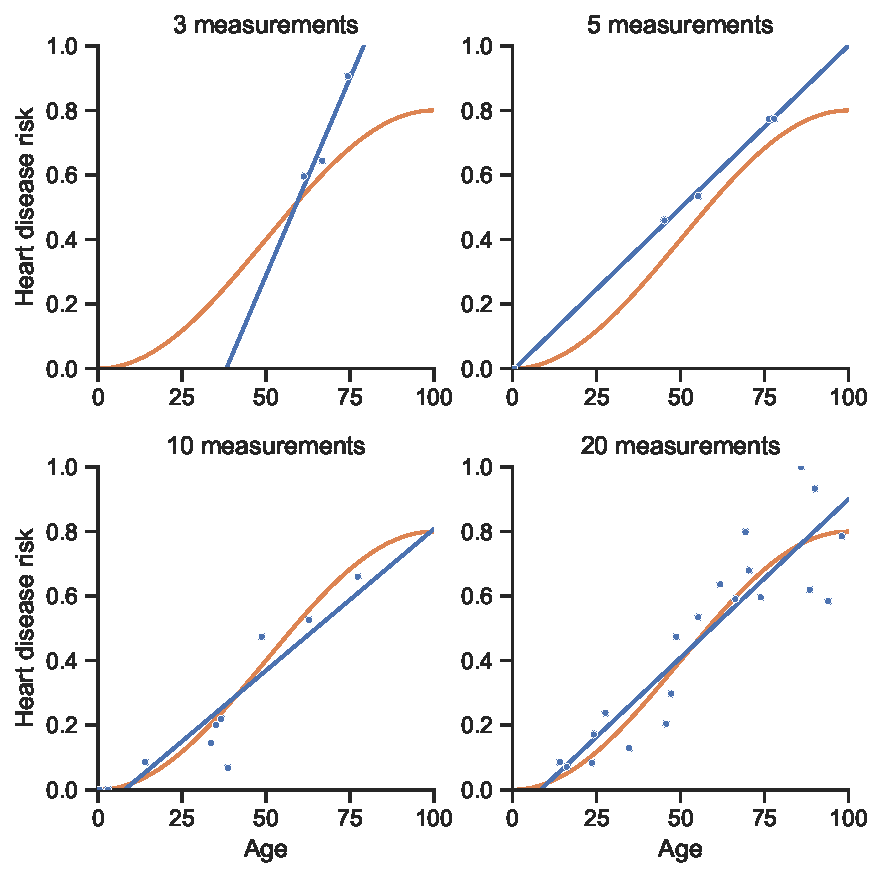
\includegraphics[width=0.5\linewidth]{images/3/heart_disease_risk_samples}}
 \hfill
 \caption{A simulated example of heart disease risk prediction using simple linear regression. The plots on the right show how the approximated function depends on the sample size.\label{fig:t1-t2-example}}
\end{figure}

The simulation with only three points clearly demonstrates a mismatch between the approximated and underlying functions. This discrepancy is known as \textbf{overfitting}. Overfitting occurs when the model is overly influenced by the specific sample of data, particularly the noise, and fails to generalize to new, unseen examples. As the number of samples increases, the approximated function aligns more closely with the underlying one. However, even with 20 measurements, there is a notable difference between the approximated and underlying functions. The underlying function is a non-linear cosine function. No matter how many data points we use, a line cannot perfectly approximate this non-linear function. This is an example of \textbf{underfitting}, where the model lacks sufficient parameters to capture the complexity of the underlying function.

To address underfitting, a more complex model is required, meaning we need a broader class of functions for optimization. Our current regression can be viewed as fitting a polynomial function to the dataset. Initially, we have employed polynomials of degree 1 — lines. We can generalize our model to an $n$-degree polynomial:

\begin{equation}
	f(x) = \theta_n x^n + \theta_{n-1}x^{n-1} + \cdots + \theta_1 x + \theta_0.
\end{equation}

To increase our function class, we will choose a larger polynomial degree and again minimize the mean squared distance to obtain $\theta_n$ through $\theta_0$. By increasing the degree we are increasing the complexity of the model and the model will be able to represent more complex underlying functions. We can observe what happens when we choose degrees 2, 3, or 5 in \figref{fig:reg-deg-2}.

\begin{figure}[h]
 \centering
 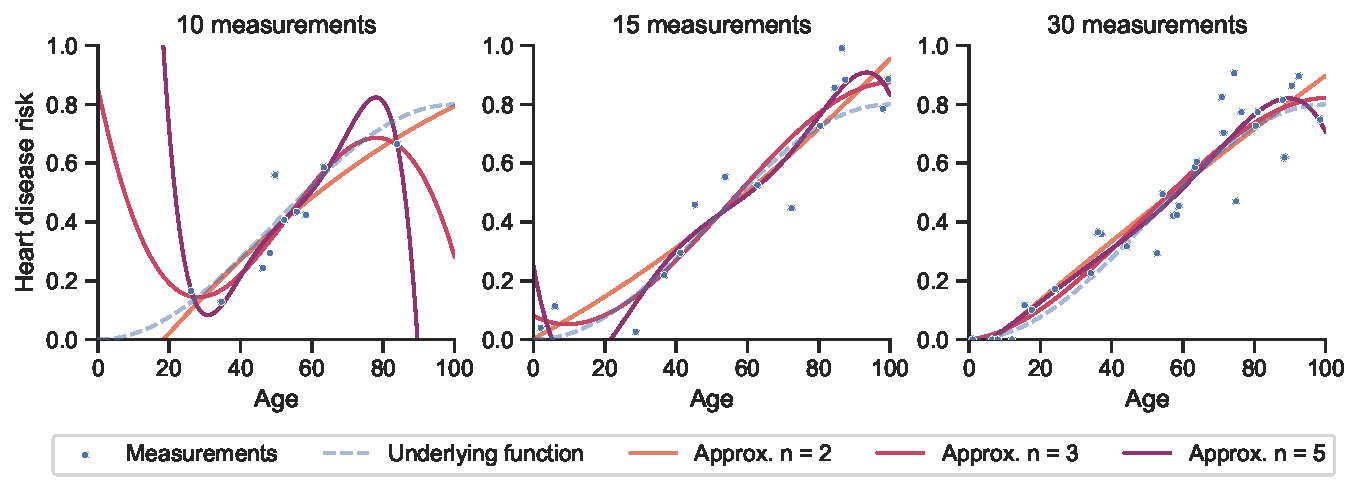
\includegraphics[width=\columnwidth]{images/3/heart_disease_risk_samples_degrees}
 \caption{Fitting a polygonal function of various degrees on three different sample sizes.}
 \label{fig:reg-deg-2}
\end{figure}

In the case with 10 measurements, we observe that the approximated polynomial with $n = 2$ follows the underlying function somewhat well. However, as we increase the degree the function quickly begins to overfit. This experiment demonstrates that the likelihood of overfitting increases with model complexity. Yet, we need complex models to approximate complex functions.

This inherent conflict between overfitting and underfitting is known as the \textbf{bias--complexity tradeoff} (alternatively, the bias–-variance tradeoff). Let us investigate this problem more formally. We can decompose the error of a deep learning model into two components \cite{shalev-shwartzUnderstandingMachineLearning2014}. Consider a trained model $f_\theta$ with optimal parameter values $\theta$ from a class of functions $\mathcal{F}$. Let there be a function $L(f)$ that measures the error between any model $f \in \mathcal{F}$ and the underlying function we are approximating. The total error of the trained model can be expressed as:

\begin{equation}
	L(f_\theta) = \epsilon_{app} + \epsilon_{est}
	\text{ where:\;}  \epsilon_{app} = \min_{f \in F}L(f),\;
	\epsilon_{est} = L(f_\theta) - \epsilon_{app},
\end{equation}

where $\epsilon_{app}$ is the \textbf{approximation error} and $\epsilon_{est}$ is the \textbf{estimation error}. The approximation error is the residual error when using the best possible approximator within our chosen class of functions $\mathcal{F}$. In other words, the error that remains given the best possible model parameters. For instance, in the earlier function approximation example with a 1st-degree polynomial, even with infinite data, there would always be some discrepancy in approximation compared to the underlying function. The approximation error depends entirely on the class of functions we use and can only be reduced by adopting a different class, such as polynomials of a higher degree. The remaining estimation error depends on the quality of our parameters $\theta$. It is possible to have a class of functions capable of perfectly approximating the underlying function but still fail to precisely identify the optimal function within that class.

In our previous experiment, we observed that the estimation error is influenced by both the sample size and the complexity of the model. To formally analyze this, we can explore the concept of \textbf{sample complexity}. Sample complexity, denoted as $n(\epsilon, \delta)$ for chosen $\epsilon, \delta \in (0, 1)$ measures the number of samples needed for a model $f$ chosen from a finite class of functions $\mathcal{F}$ to be \textbf{probably approximately correct}. This means that, across different samplings of data points, there is a probability of $1 - \delta$ that the model is correct within some margin of error $\epsilon$, i.e. $L(f) \leq \epsilon$. Assuming there exists some unknown $f' \in \mathcal{F}$ for which $L(f') = 0$, we can say that the approximation error is zero. Then, it can be shown \cite{shalev-shwartzUnderstandingMachineLearning2014} that:

\begin{equation}
	n(\epsilon, \delta) \geq \frac{\log(\lvert \mathcal{F} \rvert \delta)}{\epsilon}.
\end{equation}

We can see that an increased function class size (for instance, by choosing a higher-degree polynomial) necessitates a larger sample size $n$ to probably approximately correctly approximate the underlying function. Thus, we conclude that the estimation error can be reduced either by adding more data samples or by decreasing the size of the function class we are optimizing over.

In medical image segmentation, we have an unfortunate stalemate between the three factors governing estimation and approximation errors. The complexity of medical image segmentation demands a large number of parameters, which in turn increases the estimation error. Ideally, this error could be mitigated by adding more data samples, but in the realm of medical imaging, acquiring ample data is often impractical.

To reduce the estimation error, we are left with reducing the size of the function class. We can do so in two ways. The first involves reducing the parameters of the model itself, shrinking the class of functions, and allowing the model to more easily find the optimal function. This usually requires transforming the data such that it can be easily segmented with a less complex model, or using domain-specific knowledge to reframe the problem. The second method involves initializing the model with parameters that are already near-optimal. In this case, the model starts close to the optimal function, needing only to search within a local space around these parameters. This is typically achieved by first optimizing the model on similar data for a related task that involves learning features pertinent to segmentation, followed by further optimization for the specific segmentation task.

In the subsequent sections, we will delve into specific techniques from these two approaches, providing examples of their application in neural network-based medical image segmentation.

\section{Transfer Learning}

Consider the task of segmenting liver tumors in CT scans. Suppose we have a limited dataset of labeled liver tumor regions, but a more extensive collection of labeled liver regions. In such a scenario, the first step would be to train a neural network for liver segmentation. The rationale here is that most of the parameters learned for liver segmentation will be relevant and close to those needed for liver tumor segmentation. Therefore, when we are developing the liver tumor segmentation network, we copy the values of the parameters learned in the liver segmentation network. We can then say that the network was \textbf{pre-trained} or \textbf{initialized} on a liver segmentation dataset and \textbf{fine-tuned} on the liver tumor segmentation dataset.

In this thesis, we refer to this basic technique as ``simple transfer learning''. There are many other more complex ways of achieving pre-training and fine-tuning. In this section, we will present an overview of some of these methods.

	\subsection{Simple Transfer Learning}
	
	Simple transfer learning is a prevalent technique in medical image segmentation. Typically, segmentation neural networks in this field are initialized with weights trained on the ImageNet dataset \cite{dengImageNetLargescaleHierarchical2009a}. ImageNet comprises a collection of natural images, which significantly differ in distribution from medical images. As a result, initializing with ImageNet-trained weights doesn't usually enhance accuracy but it does make the network converge faster. This is because such initialization 'skips' the phase of learning fundamental image features that are common across various types of images, including medical ones. Figure \ref{fig:stl-diagram} illustrates this process.
	
Simple transfer learning is used extensively in medical image segmentation. Segmentation neural networks are commonly initialized using weights trained on the ImageNet dataset \cite{dengImageNetLargescaleHierarchical2009a}. ImageNet is a dataset of natural images and its distribution is drastically different from medical images. Therefore, this initialization does not typically lead to increases in accuracy but can make the network converge faster as it ``skips'' having to learn to detect base-level image features common to all images. This process is shown in \figref{fig:stl-diagram}.

\begin{figure}[h!]
 \centering
 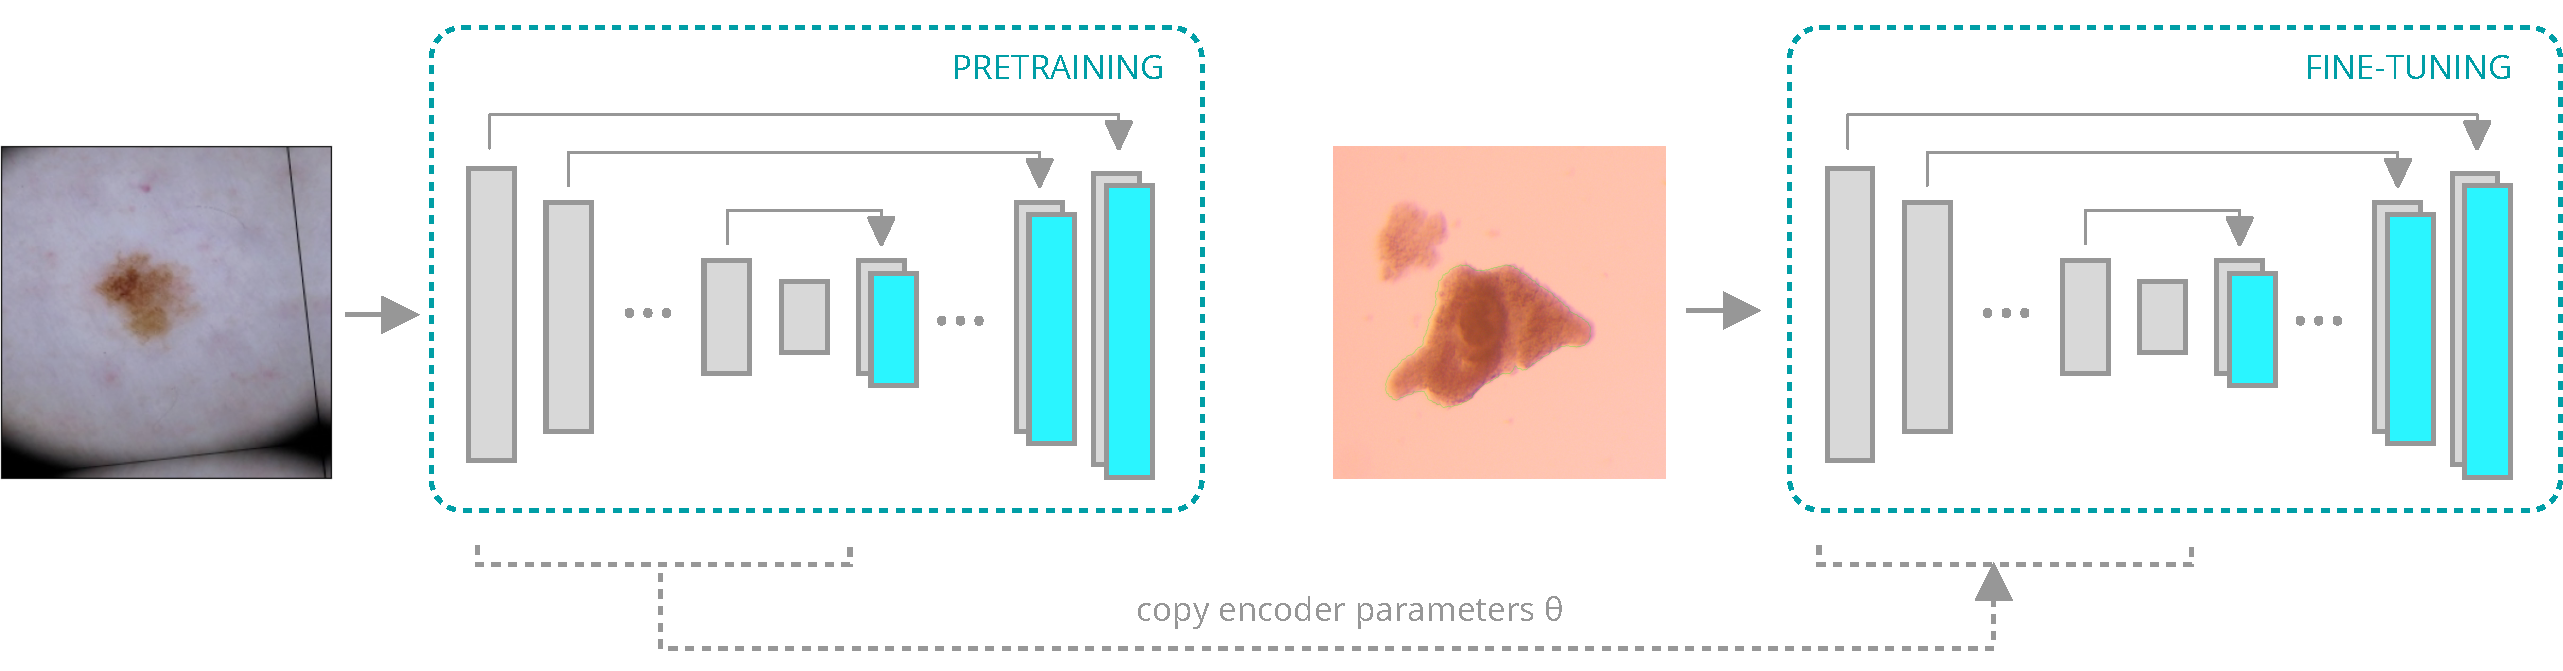
\includegraphics[width=\linewidth]{images/3/simple-transfer-learning-diagram}
 \caption{An overview of the simple transfer learning procedure. First, a model is pretrained on some related segmentation task. Then, part of the trained model's weights are copied to a new model that is then fine-tuned on the target segmentation task.}
 \label{fig:stl-diagram}
\end{figure}

Recent datasets, like \citet{wasserthalTotalSegmentatorRobustSegmentation2023}, comprising over 1000 subjects, are increasingly utilized for transfer learning, improving the accuracy of downstream tasks \cite{monaiconsortiumMONAIMedicalOpen2023, myronenkoAutomated3DSegmentation2023}. While these approaches can result in impressive performance improvements, their application is constrained to fields where ample, similar data is accessible. In more specialized modalities or segmentation problems, the knowledge learned during pre-training may not be adequate for improving downstream accuracy.  A potential solution to bridge this gap involves adapting the pre-trained model to the specific target domain, a topic we'll explore in the following section.

	\subsection{Domain Adaptation}
	
Neural networks often struggle to generalize across different datasets, even within similar domains \cite{torralbaUnbiasedLookDataset2011}. This is referred to as the ``domain shift'' problem. Overcoming this problem could lead to an increase in data efficiency since a model trained on some similar large dataset can perform well on a smaller target dataset. Various domain adaptation techniques have been developed to tackle this challenge.

One class of methods aims to explicitly penalize domain shift by including an estimate of domain shift in the loss function. For instance, \citet{liuUnsupervisedDeepDomain2018} first train a network on a source domain with abundant data. This network is then adapted to perform segmentation on a target domain with limited data. During adaptation, the loss function includes a term for the maximum mean discrepancy between the encoded feature vectors of the source and target domains. Minimizing this term forces the encoder to maintain consistent feature representations rather than shifting the distribution of the encoded feature maps.

Another approach involves reducing the network's ability to distinguish between source and target domains, thereby removing information that leads to domain shift. \citet{ganinDA2015} add a classification head to the network to identify the input's domain. Typically, networks adjust their parameters to minimize loss during each iteration. However, in \cite{ganinDA2015}, the gradients from the domain classifier are inverted so the network updates its parameters to make it harder to differentiate between the two datasets. This method is illustrated in \figref{fig:unsup-dom-adpt}.

\begin{figure}[h!]
 \centering
 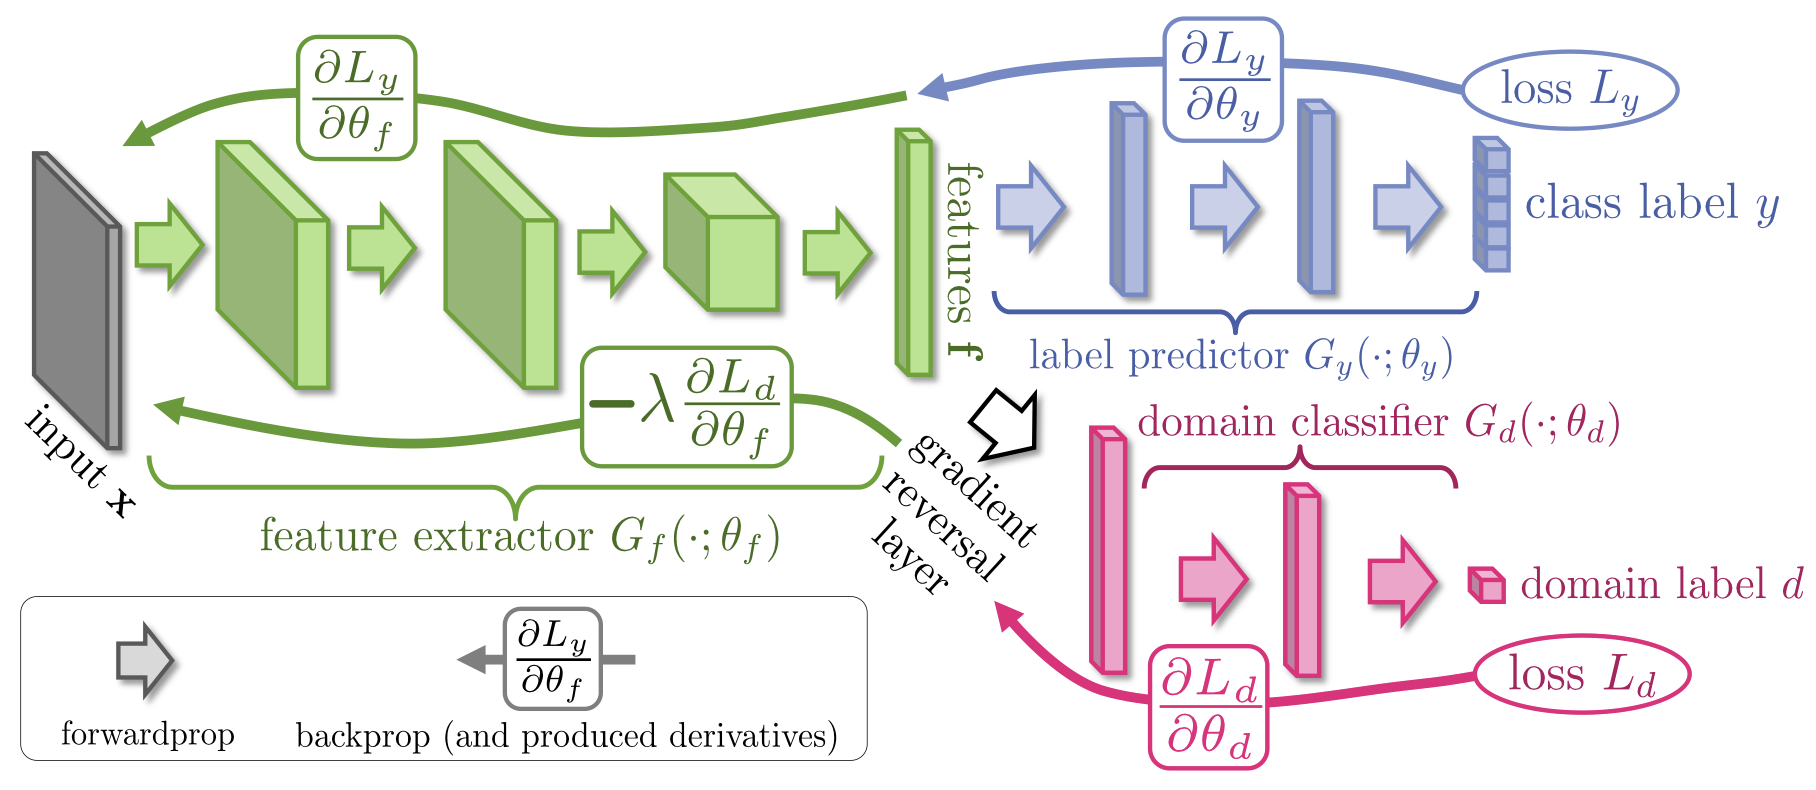
\includegraphics[width=0.7\linewidth]{images/3/unsup-dom-adpt}
 \caption{A diagram of the domain adaptation approach in \citet{ganinDA2015}. The gradients of the domain classification head which are applied to the encoder are reversed during backpropagation.}
 \label{fig:unsup-dom-adpt}
\end{figure}
	
Domain adaptation has been effectively applied to medical image segmentation, as demonstrated in the work of \citet{bermudez-chaconDomainadaptiveTwostreamUNet2018}. They utilized a U-Net-like architecture with dual encoder branches, each processing images from a different domain, paired with a shared decoder. Their loss function incorporates a maximum mean discrepancy term, comparing the decoder’s final feature maps from inputs of both domains. This method was employed for segmenting mitochondria and synapses in microscopic images.

Although domain adaptation techniques enhance transfer learning performance, they generally require labeled data from the source domain. There is growing interest in methods that can utilize unlabeled data to identify general features in images from the target domain regardless of the specific task. We'll explore these methods in the following section.

	\subsection{Semi-Supervised and Self-Supervised Learning}
	
Semi-supervised learning combines both labeled and unlabeled data to train neural networks. One such approach is \textbf{self-supervised learning}, where a feature extractor can be trained in a completely unsupervised manner using a large number of images. Then, that feature extractor can employed via transfer learning to train a network for some specific task such as segmentation. One common strategy for this involves a \textbf{pretext task}, where the network is trained on a task for which solutions can be automatically generated from unlabeled data, using automatically generated labels to train the network. A pretext task could be, for instance, solving jigsaw puzzles \cite{norooziUnsupervisedLearningVisual2016}. An image is divided into $3 \times 3$ tiles, the tiles are randomly shuffled and fed into the network. The network is tasked with reordering these tiles to reconstruct the original image. Solving this task forces the network to learn to identify salient features such as recognizing a single object across multiple tiles. Such an approach is visualized in \figref{fig:ssl-pretext}.

\begin{figure}[h!]
 \centering
 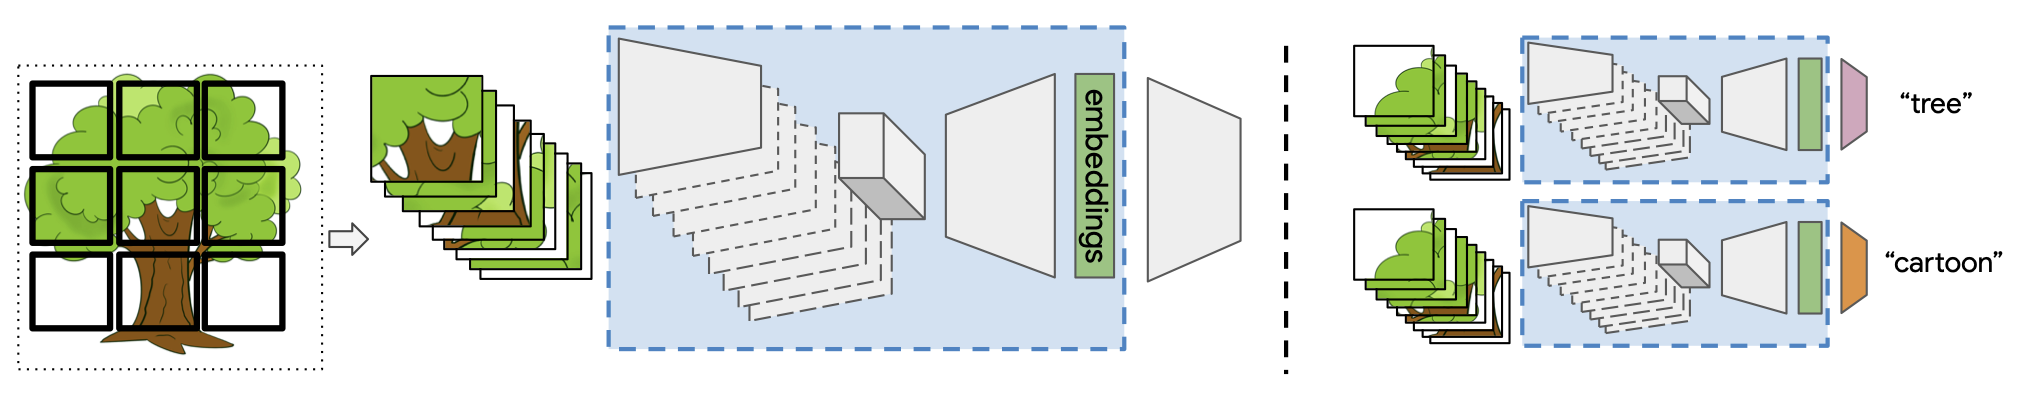
\includegraphics[width=\linewidth]{images/3/shuffle-to-learn}
 \caption{A self-supervised learning approach using shuffling image tiles as a pretext task presented by \citet{carr2021shuffle}. The trained feature encoder learns to extract relevant features and its parameters are transferred to a model trained to perform the downstream task.}
 \label{fig:ssl-pretext}
\end{figure}

Recently, a more common approach to self-supervised learning is \textbf{contrastive learning}.
This approach focuses on training the encoder to minimize the distance between feature vectors of similar (or positive) examples while maximizing the distance between dissimilar (or negative) examples. Positive examples are generated in an unsupervised manner, often by applying random augmentations to an image to create two variants.  The goal is for the feature vectors of these variants to be closely aligned. This teaches the network to recognize similar objects in a way that is invariant to the augmentations. Notable implementations of contrastive learning include SimCLR \cite{chenSimpleFrameworkContrastive2020} and MoCo \cite{he2019moco}.

\section{Synthetic Data}

The data efficiency methods we've discussed so far revolve around pre-training networks with unlabeled or similar data. An alternative strategy involves generating synthetic data that mimics the target distribution. There are various techniques for this, each offering different levels of complexity and generation quality. A straightforward and commonly used method for expanding dataset size is \textbf{data augmentation}.

\textbf{Data augmentation} refers to the application of random transformations to input images, thereby artificially increasing their diversity. These transformations can be simple ones such as adjusting brightness or contrast, flipping the image horizontally, or more intricate, involving complex random deformations of the image. Generally, the choice of transformations is governed by domain knowledge --- the network is forced to disregard transformations that we know it should be invariant to. Data augmentation is a standard practice in segmentation models, often employed alongside other data efficiency techniques. However, its implementation typically relies on simple deformation or transformation methods, which limits its capacity to create truly diverse samples.

Recently, the field of deep learning-based image generation, especially generative adversarial networks and diffusion models, has sparked a large interest in generating synthetic medical images. \textbf{Generative adversarial networks} \cite{goodfellowGenerativeAdversarialNetworks2014} consist of two neural networks, a generator and a discriminator, that are trained simultaneously. The generator creates synthetic images intended to be indistinguishable from real images, while the discriminator learns to differentiate between the two. The process continues until the generator produces images so convincing that the discriminator cannot easily distinguish them from real images. This technique has been particularly effective in generating realistic medical images for data augmentation \cite{shinMedicalImageSynthesis2018}.

Diffusion models \cite{ho2020denoising}, a more recent development in the field of generative models, offer an alternative approach to image generation. These models, inspired by the physical process of diffusion, work by gradually adding noise to an image and then learning to reverse this process. The result is the generation of new images by reversing the noise addition process from a randomly sampled noise distribution. Diffusion models have been shown to generate high-quality images that can be particularly useful in medical imaging contexts \cite{khaderDenoisingDiffusionProbabilistic2023}.

\subsection{Conclusion}

As we have seen, there are several approaches to increasing the data efficiency of neural network-based segmentation of medical images. This thesis focuses on using regularisation by transforming the input data in such a way as to allow the network to use fewer parameters to achieve its segmentation task. We do so by combining predictions of neural networks with more traditional approaches from image processing and data augmentation. In the next chapter, we will introduce this idea and some specific applications.


\printbibliography[heading=subbibintoc]
\end{refsection}

\begin{refsection}
% Kapitel 3

\chapter{Data Efficiency via Model-Driven Preprocessing}
\label{chap:model-driven-preprocessing}

In this chapter, we will propose another way of achieving data efficiency in neural network-based medical image segmentation. Our approach centers on preprocessing the input data using domain knowledge and traditional image-processing techniques to make the image more easily segmentable. However, instead of manually selecting transformation parameters, we will model the parameters as functions of the image, and train a neural network to estimate optimal transformation parameters. As discussed in the previous chapter, regularization enables a network to limit its number of parameters to what is necessary for the given problem's complexity. Through strategic image transformation, we aim to simplify the complexity of the segmentation task, thus allowing for efficient segmentation with fewer parameters.

 We will first present some motivation to show how it is possible to transform data to be easier to model. This is followed by a detailed outline of our method, as well as an empirical study, demonstrating the effectiveness of our approach across various medical image segmentation tasks. We then show an improvement of the method to support multiple segmenting objects and another empirical study using the improved approach.

\section{Motivation: Using The Polar Transform for Preprocessing}

Our approach is centered on discovering transformations of data that enable neural networks to approximate decision boundaries with fewer parameters. This strategy is grounded in a particular interpretation of neural networks. Consider a network tasked with classifying a given image region \(I(x, y)\) as class ``0'' or ``1''. All conceivable image regions \(I(x, y)\) form part of a \(d\)-dimensional space, known as the input space. Here, \(d\) represents the total number of pixels in the region multiplied by the number of channels in each pixel. The neural network, through iterative optimization, seeks to transform the input space into some other $n$-dimensional in such a way that it becomes linearly separable by an $n$-dimensional hyperplane into two distinct classes. This process and its outcome are depicted in \figref{fig:input-space-transform}.

	\begin{figure}[h]
		\centering
		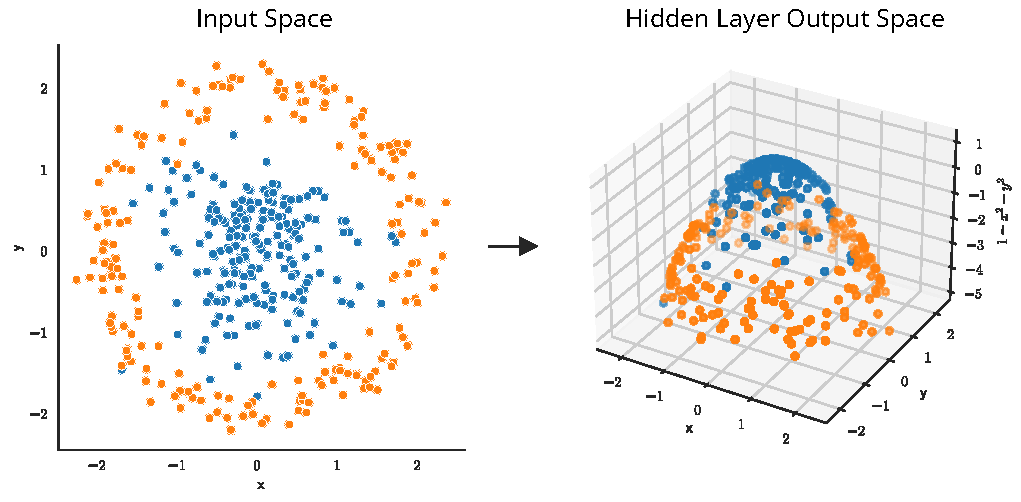
\includegraphics[width=0.65\linewidth]{images/4/nn_trans_dataset}
		\caption{An example of how a 2-class classification neural network bends an input space (left) such that it is linearly separable with a hyperplane.}
		\label{fig:input-space-transform}
	\end{figure}

To find the transformation, the network needs a sufficient number of parameters. More parameters allow for more complex transformations. For instance, to accurately approximate a circular decision boundary, the network needs at least three neurons in its second layer. We exemplify this in \figref{fig:circ-datataset-neurons}.

	\begin{figure}[h]
		\centering
		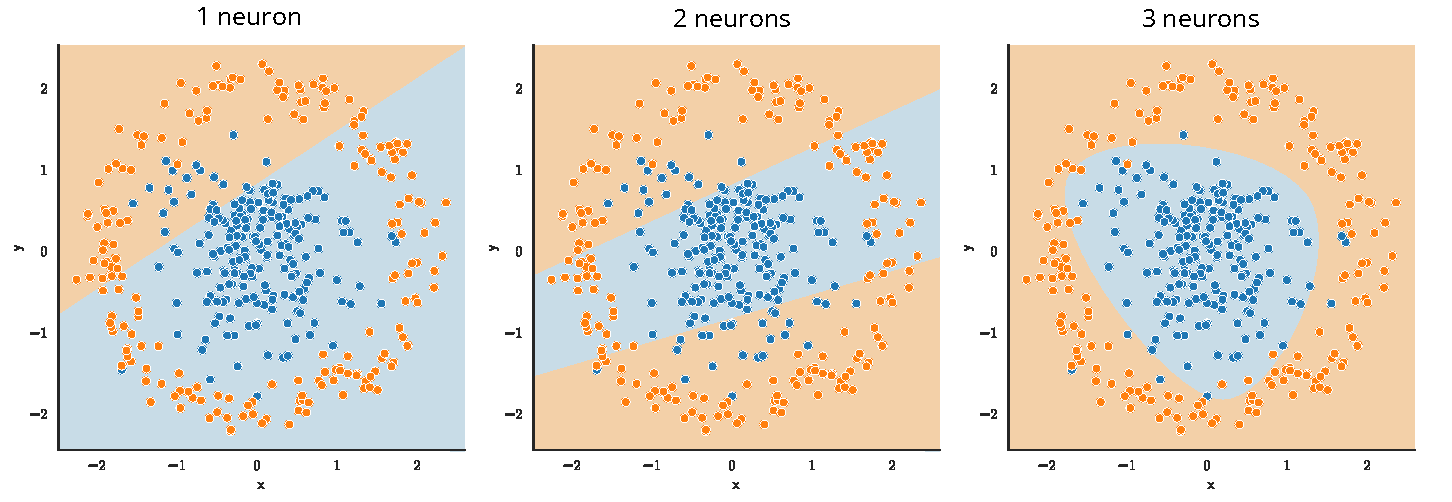
\includegraphics[width=\linewidth]{images/4/circular_dataset_neurons}
		\caption{The decision boundary (shown as the background color) according to a fully connected neural network with three layers where the second layer has one, two, or three neurons.}
		\label{fig:circ-datataset-neurons}
	\end{figure}

% The essence of data efficiency in neural networks is to establish a decision boundary using fewer data samples. This is achieved by narrowing the search space of the function class or, in simpler terms, reducing the number of parameters within the neural network. In the current and subsequent chapters, our focus will be on devising methods to pre-process the data into an intermediary form, denoted as \(\mathcal{X}_{pre}\), which is more easily separable than the original input space \(\mathcal{X}\). By transforming data into \(\mathcal{X}_{pre}\), which is closer to the ideal transformed space \(X'\), the network requires fewer parameters as it has a smaller search space to find \(X'\). This transformation process is referred to as \(\mathcal{T}\).

% A prime example of such a transformation is the polar transform. Specifically in two dimensions, the polar transform \(\mathcal{T}(X_i; C)\), defined by a chosen origin \(C = [c_0, c_1]\), converts an input vector \(X = [x_0, x_1]\) into a vector \(\mathcal{T}_C(X) = [\theta, r]\). The transformation is as follows:

The goal of data efficiency is to find a decision boundary given fewer data samples. As discussed in the previous chapter, this necessitates narrowing the search space of possible decision boundaries, or, in other words, reducing the number of neural network parameters. In the current and subsequent chapters, our focus will be on devising methods to pre-process the data into an intermediary form, denoted as \(\mathcal{X}_{pre}\), which is more easily separable than the original input space \(\mathcal{X}\). By transforming data into \(\mathcal{X}_{pre}\), the network requires fewer parameters as it has a smaller search space to find \(X'\). This transformation process is referred to as \(\mathcal{T}\).

A commonly used example of $\mathcal{T}$ is the polar transform. In the two-dimensional case, the polar transform \(\mathcal{T}(X_i; C)\), defined by a chosen origin \(C = [c_0, c_1]\), converts an input vector \(X = [x_0, x_1]\) into a vector \(\mathcal{T}_C(X) = [\theta, r]\). The transformation is as follows:

\begin{equation}
    \begin{aligned}
	r =& \sqrt{(x_0 - c_0)^2 + (x_1 - c_1)^2},\\
	\theta =& atan2(x_1 - c_1, x_0 - c_0).
    \end{aligned}
\end{equation}

The polar transform effectively converts a circular decision boundary into a linear one. This transformation enables linear separability in our example dataset, which then requires only a single neuron in the second layer for effective classification. This is demonstrated in \figref{fig:polar_dataset_neurons}.

	\begin{figure}[h]
		\centering
		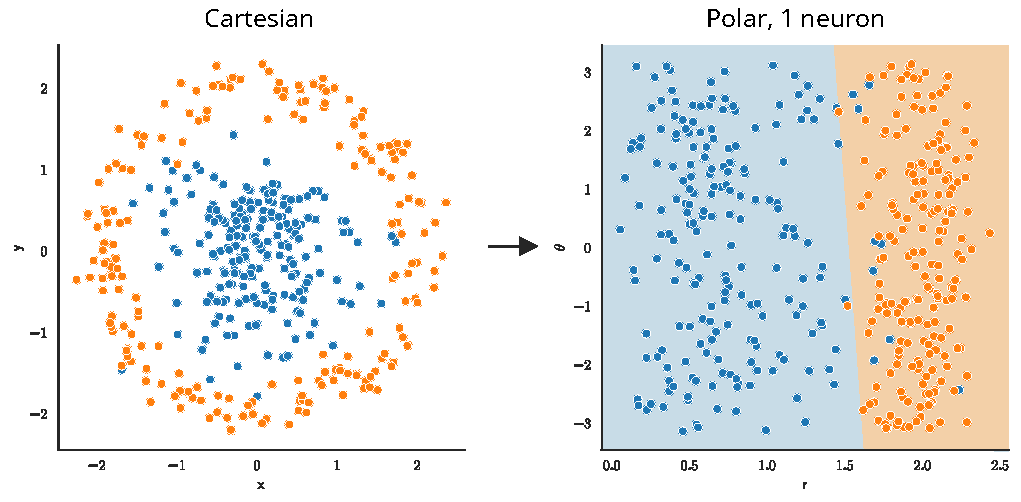
\includegraphics[width=0.65\linewidth]{images/4/polar_dataset_neurons}
		\caption{An example circular dataset transformed using the polar transform. The background color shows the decision boundary of a fully connected network with one neuron in the second layer.}
		\label{fig:polar_dataset_neurons}
	\end{figure}
	
However, the key to the polar transform's success in facilitating separability lies in the correct selection of the polar origin. When the origin is shifted away from the center of class ``0'', the decision boundary in the polar space ceases to be linear. This effect of origin displacement on the linearity of the decision boundary in the polar space is illustrated in \figref{fig:polar-origin-selection}.

 	\begin{figure}[h]
		\centering
		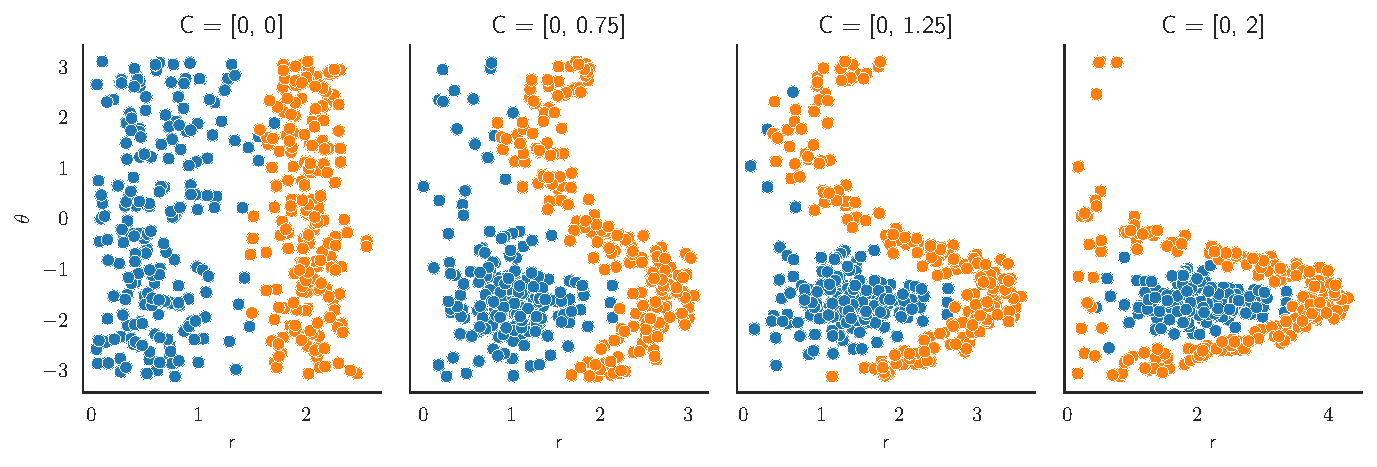
\includegraphics[width=\linewidth]{images/4/data_polar_origin}
		\caption{The polar transformation of the simulated data using different polar origins ($C$).}
		\label{fig:polar-origin-selection}
	\end{figure}
	
	Building on the example of the polar transform, we propose a methodology where key transformation parameters, like the polar origin, are dynamically estimated using a neural network. We call this approach model-driven preprocessing, specifically tailored to enhance data efficiency in medical image segmentation.
	
\section{Model-driven Preprocessing}

The concept illustrated with the polar transform can be effectively applied to image segmentation. Imagine an image where pixels belonging to one class form a circular pattern, with the background occupying the space outside this circle. A segmentation model tasked with this scenario needs to approximate a circular boundary to segment the image accurately. By applying the polar transform, this circular boundary is converted into a linear one, significantly simplifying the task and allowing for segmentation with a less complex model.

We propose a general formulation of this approach, wherein images are transformed to be more linearly separable using carefully selected transformations derived from traditional image processing methods. The success of these transformations hinges on the correct selection of parameters. To address this, we employ neural networks trained specifically to predict these optimal transformation parameters. The preprocessed image is then segmented using a regular neural network. Importantly, since the preprocessed image is inherently simpler to segment, the segmentation network can be designed with fewer parameters compared to a network segmenting unprocessed images. This is, in essence, a model-driven approach to preprocessing the image. A visual summary of this approach is shown in \figref{fig:visual-summary-mdp}. In the remainder of this section, we will describe this approach in more detail.

 	\begin{figure}[h]
		\centering
		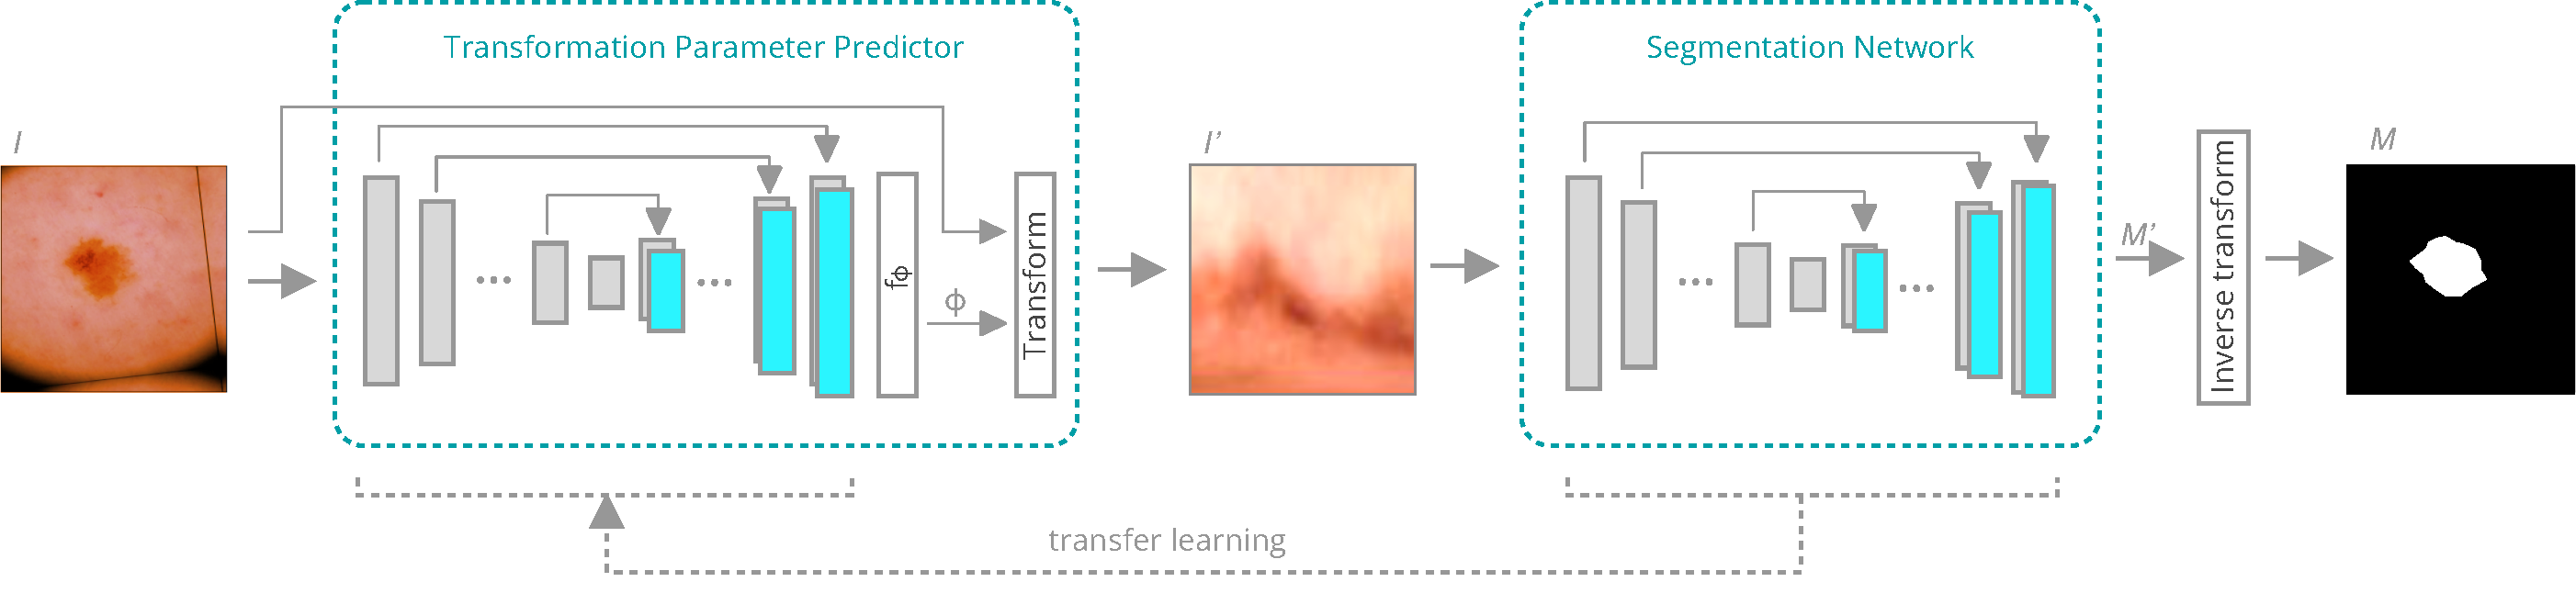
\includegraphics[width=\linewidth]{images/4/model-based-preprocessing-overview}
		\caption{A visual summary of the model-driven preprocessing approach. First, the transformation parameter predictor network predicts a segmentation-like map, from which the transformation parameters are calculated using a transformation parameter function. Then, the input image is transformed and the transformed representation is segmented by a segmentation neural network. The final segmentation map is obtained by inverting the transformation.}
		\label{fig:visual-summary-mdp}
	\end{figure}

To preprocess the image, we select a transformation function \(\mathcal{T}_{\phi}(I)\), where \(\phi\) represents the transformation parameters, and \(I\) is the original image. This transformation yields a new image, \(I'\), which can be segmented with fewer parameters than the original. 

The transformation function \(\mathcal{T}\) can vary, encompassing affine transformations, deformation fields, thresholding techniques, and, as previously mentioned, the polar transform. The choice of \(\mathcal{T}\) is contingent upon the specific segmentation task. For instance, the polar transform is advantageous for segmenting elliptical objects. When segmenting small objects, we might opt for an affine transformation that scales each object to a uniform scale. The design of \(\mathcal{T}\) should be informed by domain knowledge and validated through empirical testing. An important requirement is that \(\mathcal{T}\) must be invertible, allowing the resulting segmentation mask to be mapped back to the original image space. The segmentation process on the transformed image can be represented as:

\begin{equation}
	M(I) = (\mathcal{T}_{\phi}^{-1} \circ F_{seg} \circ \mathcal{T}_{\phi})(I),
\end{equation}

where $M(I)$ is the resulting segmentation mask for image $I$, $F_{seg}$ is the segmentation neural network. 

The effectiveness of preprocessing is highly dependent on the appropriate choice of \(\phi\), as illustrated with the polar transform. It's also important to note that \(\phi\) is specific to each image: the origin, scale, location, and distribution of objects differ across images. Acknowledging this, we propose training a model to estimate the optimal \(\phi\) for a given image:

\begin{equation}
	\phi(I) = F_{\mathcal{T}}(I; \theta_{\mathcal{T}}),
\end{equation}

where $F_{\mathcal{T}}$ is a neural network with parameters $\theta_{\mathcal{T}}$ trained to estimate the correct parameters for $\mathcal{T}$ given an image $I$. In our approach, we use various types of neural networks as $F_{\mathcal{T}}$, though it is also possible to use more traditional approaches.

More precisely, $F_{\mathcal{T}}$ is structured similarly to a regular segmentation network, producing a segmentation mask $M_\phi(I)$ in its second-to-last layer. The final layer, which is a non-trainable function $\phi(I) = f_\phi(M_\phi(I))$, produces segmentation parameters given a predicted segmentation map. $F_{\mathcal{T}}$ can then be expressed as:

\begin{equation}
	F_{\mathcal{T}}(I; \theta_{\mathcal{T}}) = f_\phi(F_{\mathcal{T}seg}(I; \theta_{\mathcal{T}})),
\end{equation}

where $F_{\mathcal{T}seg}$ is the segmentation sub-network producing $M_\phi(I)$. $F_{\mathcal{T}seg}$ can be trained using segmentation-like loss functions, where $M_\phi$ can be compared to a ground truth segmentation mask $M_{gt}(I)$. 

The function $f_\phi$ is hand-constructed using knowledge of the transformation. For instance, we know that for the polar transform, the optimal origin lies in the center of the object. Therefore, we may use the centroid of the ground truth segmentation labels as $f_\phi$. Other examples of \( f_\phi \) for various transformations include:

\begin{itemize}
	\item \textbf{CT Thresholding}: The transformation parameters are the maximum and minimum Hounsfield units representing a specific tissue. The function \( f_\phi \) could use the minimum and maximum values within the predicted segmentation mask to determine these parameters.
	\item \textbf{Rescaling}: For rescaling transformations, the parameters are the \( x \) and \( y \) scaling factors. We can determine these factors using the predicted segmentation mask to ensure that the object attains a predefined fixed width and height.
	\item \textbf{Translation}: The translation parameters, in terms of \( x \) and \( y \) shifts, can be calculated by measuring the distance between the object's center and a desired reference point.
\end{itemize}

It's important to note that \( M_\phi(I) \) doesn't have to be a conventional segmentation mask. Depending on the requirements for predicting optimal transformation parameters, we can create pseudo-labels that are more suitable for the task. For example,
 in cases where transformation parameters are contingent on an object's centroid, \( M_\phi(I) \) could be modeled as a heatmap with its focus on the object's central point. This approach enables the network to learn to predict the centroids of objects rather than their boundaries. Consequently, \( f_\phi \) can determine the object's centroid by locating the pixel with the highest intensity in \( M_\phi(I) \).

Using this approach, data efficiency is achieved by reducing the total function class size when compared to a standard segmentation neural network. We do so by using two smaller neural networks instead of one large one. Since the decision boundaries of the preprocessed images are simplified, the segmentation network needs fewer parameters to model them. Transformation parameters often have a much smaller dimensionality than the segmentation mask, and therefore the network predicting transformation parameters can naturally use much fewer parameters.

The core idea of our approach is that $\mathcal{T}$ will simplify the segmentation problem such that a regularized segmentation network $F_{seg}$ will be able to perform the segmentation using fewer parameters. To effectively implement this, both \(F_{\mathcal{T}}\) (the network predicting transformation parameters) and \(F_{seg}\) (the segmentation network) require specialized training techniques, which will be elaborated in the forthcoming section.

\subsection{Training Model-Driven Preprocessing Networks}

As mentioned earlier, using the approach of model-driven preprocessing requires specific neural network training techniques. In our approach, two separately trained neural networks are used: the transformation parameter predictor $F_{\mathcal{T}}$ and the segmentation network $F_{seg}$. 

\subsubsection{Training the Transformation Parameter Predictor}

\(F_{\mathcal{T}}\) is designed to process original, untransformed images and output the corresponding transformation parameters, \( \phi(I) \). As previously discussed, the penultimate layer of \(F_{\mathcal{T}}\) generates a segmentation-like mask \( M_\phi(I) \). The training data for \(F_{\mathcal{T}}\) comprises pairs of images and their corresponding ground truth masks, represented as \((I, M_{gt})\). Given a predicted segmentation mask $M_\phi = F_{\mathcal{T}seg}(I)$ and the transformation parameter function $f_\phi(M(I))$, the transformation parameters loss $L_\mathcal{T}$ can be calculated as:

\begin{equation}
	L_\mathcal{T}(I, M_\phi, M_{gt}) = \alpha L_\phi(f_\phi(M), f_\phi(M_{gt})) + \beta L_{M}(M_\phi, M_{gt}),
\end{equation}

where $L_\phi$ measures the error in predicting the transformation parameters, while $L_{M}$ is a segmentation-like loss that measures the error in predicting the segmentation mask used to calculate the transformation parameters. The coefficients \(\alpha\) and \(\beta\), which balance these two terms, are determined empirically.

\subsubsection{Training the Segmentation Network}

The segmentation network is trained using ground-truth transformation parameters (\(\phi\)) to preprocess the input image. For every pair of image and ground truth segmentation label \((I, M_{gt})\), the ground truth transformation parameters are derived using:

\begin{equation}
	\phi = f_\phi(M_{gt}) + z_\phi,
\end{equation}

where \(f_\phi\) is the transformation parameter function, identical to the one used in the parameter predictor network. The term \(z_\phi\) represents a random noise vector matching \(\phi\)'s dimensions. This noise serves as a form of augmentation, enhancing the segmentation network's resilience to less-than-ideal \(\phi\) predictions.

Given $\phi$, the input to the segmentation network is constructed as $I' = \mathcal{T}_\phi(I)$. The network's final layer applies an inverse transformation to the output segmentation map, \(\mathcal{T}^{-1}_\phi(M)\). To train the network, we use a standard segmentation loss $L_{seg}(M, M_{gt})$.

\subsubsection{Transfer Learning}

Given that the parameter predictor mirrors the structure of a segmentation network, we can utilize the same encoder and decoder in both networks, leveraging various forms of transfer learning. This approach offers several advantages:

\begin{enumerate}
	\item Both networks employ a standard encoder, enabling the initialization of these networks with weights pre-trained on extensive medical or natural image datasets.
	\item The development process can start by training a standard baseline segmentation model on untransformed data. Subsequently, the learned weights from this model can be transferred to both the segmentation and transformation parameter predictor networks. In this case, the parameter predictor already knows how to localize the objects, thereby enhancing its ability to predict optimal transformation parameters.
	\item The transformation parameter predictor network's main role is to robustly transform input images. Domain shifts or unrealistic data, which are critical concerns for the segmentation network, are less problematic for the parameter predictor. This leniency allows for the use of extensive augmentation during training, further improving the network's robustness and adaptability.
\end{enumerate}

Having laid out the theoretical framework of this approach, the remainder of this chapter will detail a specific application of this methodology, demonstrated through an empirical study across various medical imaging datasets. This study aims to showcase the practical effectiveness and adaptability of the model-driven preprocessing approach in real-world scenarios.

\section{Model-Driven Polar Transform Using Centerpoint Prediction}
\label{polar-paper}

Earlier in this chapter, we discussed how the polar transform can simplify complex decision boundaries, making segmentation tasks more manageable. Drawing from this insight, this section introduces a practical implementation of our model-driven preprocessing approach, utilizing the polar transform. The approach involves two networks: a transformation parameter predictor and a segmentation network. In this specific implementation, the parameter predictor is designed to determine the polar origin of an image, functioning as a centerpoint predictor network. Its objective is to identify the center of a singular object within the image. We will explore two distinct designs for this centerpoint predictor network:

1. \textbf{Segmentation-like Network}: This design focuses on identifying the centroid of a segmentation mask. It operates like traditional segmentation networks but is specifically optimized to pinpoint the center of an object.

2. \textbf{Heatmap Prediction Network}: Alternatively, this network predicts the centerpoint directly as a heatmap. This approach is more direct, as it aims to localize the object's center without necessarily delineating its entire boundary.

Once the centerpoint is determined, the image undergoes a transformation using the predicted polar origin. The transformed image is then fed into a segmentation network that has been trained on images processed with the polar transform. This setup aims to demonstrate the effectiveness of preprocessing in simplifying the segmentation task, potentially allowing for more accurate and efficient segmentation with neural networks. The subsequent parts of this section will delve into the specifics of these network designs and their performance in practical scenarios.

Our method is evaluated on 
the tasks of polyp segmentation, liver segmentation, skin 
lesion segmentation, and epicardial adipose tissue (EAT) segmentation.
The proposed method can be used as a pre-processing step for 
existing neural network architectures, so we evaluate the methods using
common neural network architectures for medical image segmentation including U-Net 
\cite{ronnebergerUNetConvolutionalNetworks2015}, U-Net++ 
\cite{zhou2019unetplusplus} with a ResNet \cite{heDeepResidualLearning2016} encoder, and DeepLabV3+ \cite{chenEncoderDecoderAtrousSeparable2018} with a ResNet \cite{heDeepResidualLearning2016} encoder. Evaluation of our approach as a pre-processing step shows that it improves segmentation performance across different datasets and neural network architectures while making the networks more robust to small dataset sample sizes.

\subsection{Background and Related Work}

The polar transform's potential for simplifying the segmentation of images with elliptical borders was discussed earlier in this chapter. Transforming such images into polar coordinates effectively turns a perfect circle from Cartesian coordinates into a straight line, significantly simplifying the decision boundary. This simplification means that a less complex model can accurately predict borders in polar coordinates. As illustrated in \figref{fig:polar-lesion}, even for complex shapes, transforming roughly elliptical objects into polar coordinates can reduce the complexity required for accurate segmentation. Moreover, by using the object's center as the polar origin, the approach standardizes the location and border distances in each training example. This standardization allows the model to focus on learning the border distance from the origin at various angles, obviating the need for object localization learning.

\clearpage

	\begin{figure}[h]
		\centering
		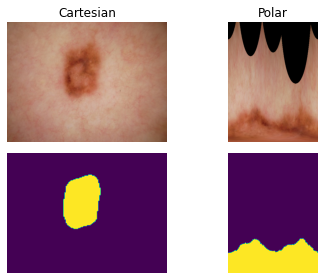
\includegraphics[width=0.4\linewidth]{images/4/to_polar}
		\caption{An example image and label from the lesion dataset and their corresponding polar transformation. \cite{bencevicTrainingPolarImage2021}}
		\label{fig:polar-lesion}
	\end{figure}

Given a polar origin $(c_x, c_y)$ of a Cartesian image $I(x, y)$ of resolution $H \times W$, we obtain each point $(r, \vartheta)$ of the polar transformed image $I'(r, \vartheta)$ as:

  \begin{equation}
    \begin{aligned}
      r &= \frac{H}{2 \pi} \cdot atan2(y, x) [ \cdot 180 / \pi ], \\
      \vartheta &= \frac{W}{\sqrt{(W / 2)^2 + (H / 2)^2}} \cdot \sqrt{x^2 + y^2},
    \end{aligned}
    \label{eq:polar-transform}
  \end{equation}
  
  where $atan2$ is the 2-argument arctangent function.

    \subsubsection{Previous work using the polar transform for medical image processing}
    
Several image segmentation methods were proposed that utilize polar coordinates. 
\citet{liuDDNetCartesianpolarDualdomain2019a} proposed an approach they
call Cartesian-polar dual-domain network (DDNet) to perform optic disc and cup segmentation
in retinal fundus images. The neural network contains two encoding branches, one for a Cartesian input image and another for the polar transformation of the same input image. The predictions are fused into a single feature vector which is then decoded into a final segmentation.
\citet{salehinejadImageAugmentationUsing2018} used the polar transformation as a way to 
augment
training data by transforming each input image into multiple polar images at various polar
origins, thus increasing the number of training data.
\citet{kimCyCNNRotationInvariant2020a} proposed a convolutional neural network layer for 
images in polar 
coordinates to achieve rotational invariance. Their cylindrical convolution layer uses cylindrically sliding windows to perform a convolution.
\citet{kimCNNBasedUGS2018} proposed a user-guided segmentation method where an expert 
selects the
point used as the polar origin. The transformed image is then
segmented using a convolutional neural network (CNN). 
\citet{estevesPolarTransformerNetworks2018a} proposed a polar transformer network for image 
classification. Note that "transformer network" here refers to spatial transformer networks 
\cite{jaderbergSpatialTransformerNetworks2016} and not attention-based networks commonly called 
transformers.
The network 
consist of a polar origin predictor and a neural network that predicts a heatmap. The centroid of the heatmap is then used as the origin for a polar transformation of the input image. The polar image is classified using a CNN. This approach is most similar to our proposed method, 
however, their approach focuses on image classification, not segmentation. Additionally, our approach differs in the ways the ground truth data is prepared, the neural network architectures, as well as other details.

While there are proposed methods that combine polar transformation with neural networks, most of them solve classification tasks. Some medical image segmentation methods use the polar transformation as a preprocessing step, however, the way they obtain the origin of the polar transformation is usually based on heuristics. To our knowledge, there is currently no work that explores using the polar transformation with a dynamic polar origin as a preprocessing step for semantic segmentation in a variety of medical image datasets.

  \subsection{Methodology}
  
All of the proposed methods rely on training a neural network model to segment polar images. To train on 
polar images, the input images need to be transformed using a polar origin which is near the center of 
the 
segmented object. The correct origin is not known ahead of time, so a prerequisite for predictions on polar
images is a method to determine the correct polar origin. We propose and 
evaluate two different methods for automatically obtaining the polar origin: (1)
estimation via a segmentation trained on non-polar images and (2) training a center-point predictor that predicts heatmaps from input images. 
This section describes these methods, as well as methods to train the 
final segmentation model on the polar images.
      
In each of our approaches, the final segmentation is done using a neural network trained on polar 
transformations of the input images. In the rest of this paper, we refer to this network as the polar 
network. In all of the described approaches, the polar transformation is not part of the network architecture itself, but happens as a preprocessing step for the polar network.
To transform each input image, the polar origin is determined as the center of mass of the 
ground truth label for that image. The center of mass of an image $I(x, y)$ is calculated by first 
calculating the spatial image moments matrix $M$, where the entry of the matrix at row $i$ and column $j$ is calculated as:

  \begin{equation}
    M_{ij}= \sum _{x,y} I(x,y) \cdot x^i \cdot y^j.
    \label{eq:moments}
  \end{equation}
  
The center of mass $(c_x, c_y)$ of the image can then be calculated as:

  \begin{equation}
    \begin{aligned}
      c_x &= M_{10} / M_{00}, \\
      c_y &= M_{01} / M_{00}.
    \end{aligned}
    \label{eq:center-mass}
  \end{equation}

Finally, to increase the model's robustness to suboptimal center point predictions, we augment the 
calculated center for training images \cite{estevesPolarTransformerNetworks2018a}. Each training image has 
a 30\% chance of varying the center's x and y coordinates by a random value in the range $(-0.05S, 
0.05S)$, where $S$ is the smallest resolution of the image, i.e. $S = min(W, H)$.
 
    \subsection{Centerpoint prediction}
    
Once the polar network is trained, inference can be done by transforming an input image to polar 
coordinates. The polar network requires choosing a center that is close to the center of mass of the 
segmented object. Because a future input image is unlabeled, the correct center needs to be inferred from 
the image. We propose two ways to accomplish this, described in this section.

   \subsubsection{(A) Training the same neural network on cartesian and polar images}
   \label{retraining-approach}
   
Our first approach is training the same neural network on cartesian and polar images. A summary of this
approach is presented in \figref{fig:retraining-diagram}. With this approach, 
the inference is done by first feeding the original Cartesian input images into a neural 
network used for segmentation. We refer to this network as the Cartesian network.
For an input image, the polar origin is calculated as the center of mass of the Cartesian network's
prediction for that input image, using \eqref{eq:center-mass}.
This polar origin is used to transform the original input image to polar coordinates, and the transformed 
image is fed
to the polar network. The output of the polar network is transformed back to Cartesian coordinates
to obtain a final segmentation. We assume 
identical architectures for both the Cartesian and polar networks. This makes applying this
framework to existing architectures very straightforward, as it does not require designing new neural 
network architectures or specific hyperparameter optimization and allows for the use of transfer learning to
initialize the networks.

	\begin{figure*}[h!]
		\centering
		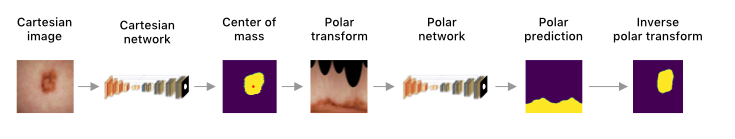
\includegraphics[width=\linewidth]{images/4/retraining-approach}
		\caption{A diagram of the approach of predicting polar origins from a Cartesian network. The first network performs an initial segmentation, which is then used to extract a polar origin for the polar transformation. The method does not rely on any specific neural network architecture. The Polar and Cartesian network can be any neural network that takes an input image and produces a binary segmentation mask as output. The red point shows the extracted polar origin. The Polar network is trained on polar image transformations. The polar transformation is not part of the network itself, but happens as a preprocessing step for the Polar network. \cite{bencevicTrainingPolarImage2021}}
		\label{fig:retraining-diagram}
	\end{figure*}
	
    \subsubsection{(B) Training a centerpoint predictor}
    \label{centerpoint-approach}
    
In the second approach for determining the optimal polar origin, we train a model specifically tasked with predicting the correct
polar origin for each input 
image, which is then used to transform the input image. The approach is shown in \figref{fig:centerpoint-approach}. 
We do this by training a neural network based on the stacked hourglass architecture 
\cite{newellStackedHourglassNetworks2016} first used for human pose estimation. Instead of training a regressor network to
predict key points in an image, the stacked hourglass architecture uses a series of stacked encoder-decoder networks, where the output
of each stack is a heatmap centered on the key point to be predicted. The output of each stack is fed as input into the next stack, allowing 
successive refinement of the heatmap prediction. During training, the loss of each stack's output is averaged to produce the final loss, 
allowing deep supervision. The final prediction heatmap is the output of the last stack in the network. To predict the center point, 
we use 8 stacked hourglass blocks, which we empirically determined as the value providing the best results. The network receives images in Cartesian 
coordinates and predicts a heatmap of the image.

	\begin{figure*}[h]
		\centering
		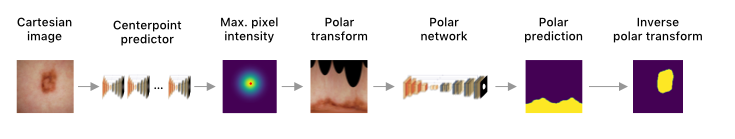
\includegraphics[width=\linewidth]{images/4/centerpoint-approach}
		\caption{A diagram of the approach of using a centerpoint prediction network. The first network can be any neural network that predicts a heatmap from an input image, which is then used to extract the polar origin, shown as a red point. The Polar network can be any semantic segmentation neural network that produces a binary mask output from an input image. The Polar network is trained on polar image transformations. The polar transformation is not part of the network itself, but happens as a preprocessing step for the Polar network. \cite{bencevicTrainingPolarImage2021}}
		\label{fig:centerpoint-approach}
	\end{figure*}
 
The ground truth heatmaps were generated by calculating the center of mass of each ground truth label 
image using \eqref{eq:center-mass}. We then create the heatmap as an image with a 2D Gaussian with the
mean on 
the center of mass on the image and a standard deviation of 8 pixels for all datasets except the liver, and 16 for the liver.
Example heatmaps are shown in 
\figref{fig:heatmap}. The optimal value for the standard deviation was determined empirically on the 
validation datasets. We found that the optimal value of the standard deviation is proportional to the size 
of the object.

	\begin{figure}[h]
		\centering
		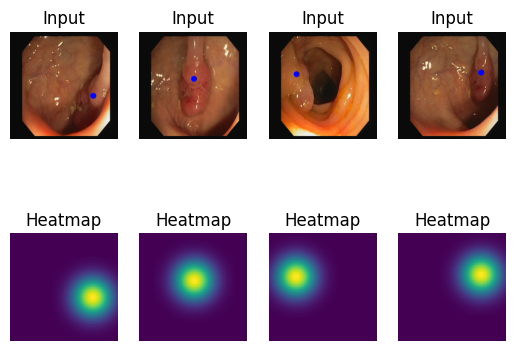
\includegraphics[width=0.8\linewidth]{images/4/heatmaps}
		\caption{Examples of heatmaps generated from the ground truth data. The heatmap is a Gaussian centered on the center of mass of the ground-truth label, shown as a blue point on the input images. \cite{bencevicTrainingPolarImage2021}}
		\label{fig:heatmap}
	\end{figure}
	
\clearpage

Additionally, during training, we use augmentation to increase the number of training inputs. In 
particular, during training for each input example, the following random augmentations are applied:

\begin{itemize}
  \item A 50\% chance of a horizontal flip.
  \item A 30\% chance of a random combination of shifting up to 6.5\% of the image dimensions, scaling up 
    to 10\% and rotating up to 45$^{\circ}$.
  \item A 30\% chance for a grid distortion, details of which are described in \cite{info11020125}.
\end{itemize}

The center-point predictor outputs 8 separate heatmaps \cite{newellStackedHourglassNetworks2016}. We
calculate the predicted center as the coordinates of the pixel with the largest intensity in the heatmap
predicted by the final layer of the model. This predicted center is then used to transform the input
image to polar coordinates, and the transformed image is fed into the polar network to perform
the segmentation. Finally, the segmentation label is transformed back to Cartesian coordinates.
    
  \subsection{Experiments} \label{experiments}
  
To validate the generality of our approach, we trained a variety of neural network architectures on 
multiple medical imaging datasets. In particular, we trained three different neural network 
architectures: U-Net \cite{ronnebergerUNetConvolutionalNetworks2015}, U-Net++ 
\cite{zhouUNetNestedUNet2018a} with a ResNet encoder and DeepLabV3+ 
\cite{chenEncoderDecoderAtrousSeparable2018a} with a ResNet encoder. Notably, each dataset we use presents a problem wherein almost all examples a single roughly elliptical object needs to be segmented. 
For each dataset and network architecture combination, we train a Cartesian and polar network, and we then 
perform four different experiments: 

\begin{enumerate}
	\item{testing the Cartesian network using Cartesian images}
	\item{testing the polar network using the ground-truth polar origin}
	\item{testing the polar network using polar origins obtained from predictions of the Cartesian network, as outlined in \ref{retraining-approach}}
	\item{testing the polar network using polar origins from the centerpoint predictor, as outlined in \ref{centerpoint-approach}}.
\end{enumerate}

    \subsubsection{Datasets description}

We used four different datasets to train the network. In this section, we give an overview of each used dataset and how it was preprocessed. Note that for training the center-point predictor, the input images were resized to a resolution of $256 \times 256$, while the generated heatmaps were resized to $64 \times 64$ pixels. Otherwise, all preprocessing steps described here are applied to the center-point model datasets as well. Each dataset was normalized and zero-centered to facilitate better network convergence. 

	\begin{figure*}
	\subfloat[Polyp dataset]{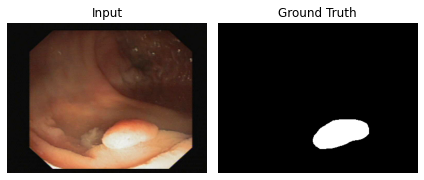
\includegraphics[width=0.49\columnwidth]{images/4/polyp_example}}
	\hfill
	\subfloat[Lesion dataset]{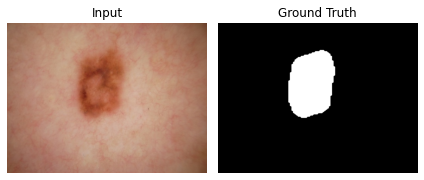
\includegraphics[width=0.49\columnwidth]{images/4/lesion_example}} \\
	\subfloat[Liver dataset]{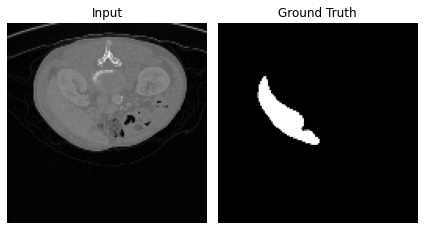
\includegraphics[width=0.49\columnwidth]{images/4/liver_example}}
	\hfill
	\subfloat[EAT dataset]{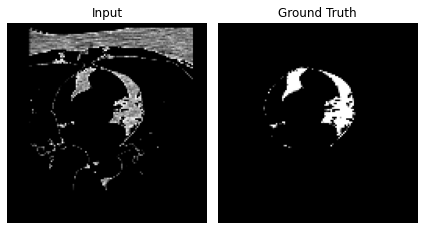
\includegraphics[width=0.49\columnwidth]{images/4/eat_example}} \\
	\caption{Example input images and ground-truth labels for each dataset used in our experiments. \cite{bencevicTrainingPolarImage2021}}
	\label{fig:datasets}
	\end{figure*}

\textbf{Polyp dataset:} The CVC-ClinicDB dataset
\cite{bernalWMDOVAMapsAccurate2015} contains 612 RGB 
colonoscopy images with the resolution $288 \times 384$ 
with labeled polyps from MICCAI 2015. We normalize each image to a range of $[-0.5, 0.5]$. 
We use the original image resolution to train all networks except the 
centerpoint network. As is used in \cite{jhaDoubleUNetDeepConvolutional2020}, 
we use an 80\%, 10\% and 10\% 
split for training, validation, and testing datasets, respectively. An example of the dataset is shown in \figref{fig:datasets}(a).

\textbf{Liver dataset:} The second dataset we use is the LiTS dataset \cite{bilicLiverTumorSegmentation2019} from the Liver Tumor Segmentation Challenge from MICCAI 2017. The dataset contains 131 CT scans of patients with hepatocellular carcinoma, with the liver as well as tumor lesions labeled by experts. In our experiments, we disregard the lesion segmentation labels and treat the dataset as a binary liver segmentation problem. In addition, we removed all slices that did not contain a ground-truth liver segmentation label, resulting in a dataset of roughly 15,000 slices. Each axial slice is thresholded to a Hounsfield scale range of $[0, 200]$ HU that contains the liver. Next, the slices are normalized to a $[0, 1]$ range and zero-centered by subtracting the global intensity of all training slices (0.1). We then proceed to train the networks on each axial slice separately. We use 101 scans for training, 15 scans for validation, and the remaining 15 scans for testing. Example liver segmentation images are shown in \figref{fig:datasets}(c).

\textbf{Lesion dataset:} The third dataset we use is the ISIC 2018 Lesion Boundary Segmentation dataset 
\cite{codellaSkinLesionAnalysis2018, tschandlHAM10000DatasetLarge2018} which contains 2,694 dermatoscopy 
images of skin lesions with expert labels of the lesions from various anatomic sites and several different 
institutions. We resize each image to a 
resolution of $384 \times 512$ and use a training, validation, and test split of 80\%, 10\%, and 10\%, 
respectively. This is consistent with \cite{jhaDoubleUNetDeepConvolutional2020}. Additionally, we normalize 
each image to a range of $[-0.5, 0.5]$. An example of a lesion 
input image and its corresponding label is shown in \figref{fig:datasets}(b).

\textbf{EAT dataset:} Finally, we also train on a dataset of labeled EAT regions from 20 patients' cardiac CT scans from 
the Cardiac Fat Database \cite{rodriguesNovelApproachAutomated2016}. The dataset has three classes labeled: 
the pericardium, EAT, and pericardial adipose tissue. We disregard all original labels except EAT and treat the dataset as a binary EAT segmentation dataset. The dataset is 
first split into training (10 patients), validation (5 patients), and test (5 patients) datasets. In the 
original dataset, 
each slice is thresholded to the adipose tissue range of $[-200, -30]$ HU and registered so that anatomical 
structures have the same locations. In addition to these original pre-processing steps, we normalize each 
slice to a $[0, 1]$ range and zero-center 
the dataset by subtracting a global mean intensity of the training set (0.1). We then train on 
each CT slice separately. An input image of the EAT dataset and its corresponding label is shown in 
\figref{fig:datasets}(d).

    \subsubsection{Implementation details}

We use the OpenCV linear polar transformation implementation.
Each model is implemented and trained using PyTorch 1.7.1 on an NVIDIA GeForce RTX 3080 GPU. For all 
networks, we use the Adam optimizer with a learning rate of $10^{-3}$. A batch size of 8 was used for all 
networks except the center-point model, where a batch size of 6 was used for the lesion and liver datasets 
and 8 for all remaining datasets. We trained all models up to a maximum of 200 epochs and used checkpoints 
after each epoch to store the model with the best validation loss. We modify the Dice coefficient to act as a loss function as shown in (\ref{eq:dice-loss}).

  \begin{equation}
    \textit{DSC}_{loss} = 1 - \frac {2\lvert X\cap Y\rvert + \lambda}{\lvert X\rvert + \lvert Y\rvert + \lambda},
    \label{eq:dice-loss}
  \end{equation}
  
where $X$ and $Y$ are the input and predicted images, respectively, and $\lambda$ is a smoothing parameter set to 1 in our experiments. 
This loss function is used to train all models except the center-point model.

The centerpoint model outputs eight heatmaps \cite{newellStackedHourglassNetworks2016}. 
We use a loss function that is the mean of the mean squared errors between each of the heatmaps and the ground truth heatmap.
The code used for all experiments is available at \url{github.com/marinbenc/medical-polar-training}.

  \subsection{Results and Discussion}

% ---------- RESULT  TABLES ---------- %

\begin{table}
\centering
\def\arraystretch{1.2}
\begin{tabularx}{\textwidth}{X X c c c c} 
 \\ [-2ex]

 \multicolumn{6}{c}{\textbf{Polyp Segmentation}}\\[1ex]
 \hline
 Architecture & Method & DSC & mIoU & Prec. & Rec. \\ 
 \hline \\ [-1.5ex]
 
 \multirow{4}{7em}{{U-Net}}
& Cartesian & 0.8315 & 0.7604 & 0.8513 & 0.8334 \\
& GT centers & 0.9484 & 0.9141 & 0.9563 & 0.9442 \\
& Cart. centers & 0.8973 & 0.8571 & 0.8996 & 0.8998 \\
& Model centers & 0.9374 & 0.8977 & 0.9488 & 0.9368 \\ [1ex]
\hline \\ [-1.5ex]

 \multirow{4}{7em}{{Res-U-Net++}}
& Cartesian & 0.8356 & 0.7636 & 0.9004 & 0.8256 \\
& GT centers & 0.9557 & 0.9260 & 0.9583 & 0.9554 \\
& Cart. centers & 0.9063 & 0.8685 & 0.9243 & 0.9027 \\
& Model centers & 0.9332 & 0.8924 & 0.9477 & 0.9321 \\ [1ex]
\hline \\ [-1.5ex]

 \multirow{4}{7em}{{DeepLabV3+}}
& Cartesian & 0.8706 & 0.8013 & 0.8857 & 0.8876 \\
& GT centers & 0.9593 & 0.9296 & 0.9576 & 0.9682 \\
& Cart. centers & 0.9212 & 0.8823 & 0.9179 & 0.9397 \\
& Model centers & 0.9338 & 0.8967 & 0.9436 & 0.9347 \\ [1ex]
\hline \\ [-1.5ex]

\multicolumn{6}{c}{\textbf{Lesion Segmentation}}\\[1ex]
 \hline
  & Method & DSC & mIoU & Prec. & Rec. \\ 
 \hline \\ [-1.5ex]
 
 \multirow{4}{7em}{{U-Net}}
& Cartesian & 0.8256 & 0.7393 & 0.8407 & 0.8712 \\
& GT centers & 0.9320 & 0.8824 & 0.9261 & 0.9541 \\
& Cart. centers & 0.8836 & 0.8317 & 0.8746 & 0.9492 \\
& Model centers & 0.9224 & 0.8699 & 0.9165 & 0.9494 \\ [1ex]
\hline \\ [-1.5ex]

 \multirow{4}{7em}{{Res-U-Net++}}
& Cartesian & 0.8664 & 0.7925 & 0.8728 & 0.9122 \\
& GT centers & 0.9439 & 0.9014 & 0.9418 & 0.9584 \\
& Cart. centers & 0.9125 & 0.8653 & 0.9075 & 0.9540 \\
& Model centers & 0.9253 & 0.8743 & 0.9253 & 0.9464 \\ [1ex]
\hline \\ [-1.5ex]

 \multirow{4}{7em}{{DeepLabV3+}}
& Cartesian & 0.8717 & 0.7984 & 0.8807 & 0.9068 \\
& GT centers & 0.9459 & 0.9059 & 0.9418 & 0.9632 \\
& Cart. centers & 0.9162 & 0.8686 & 0.9097 & 0.9536 \\
& Model centers & 0.9235 & 0.8721 & 0.9125 & 0.9570 \\ [1ex]
\end{tabularx}
\caption{Results of our proposed approaches for different tasks 
for three different neural network architectures. The Cartesian network is the network trained on Cartesian images. ``GT centers'' refers to obtaining a polar origin from the ground-truth labels and segmentation using the polar network.``Cartesian centers'' refers to predicting the polar origins from the Cartesian network and then performing segmentation using the polar network. ``Model centers'' refers to using the centerpoint predictor to obtain polar origins. (Continued on the next page.)}
\label{table:results}
\end{table}

\begin{table}
\ContinuedFloat
\centering
\def\arraystretch{1.2}
\begin{tabularx}{\textwidth}{X X c c c c} 
\\ [-2ex]
\multicolumn{6}{c}{\textbf{Liver Segmentation}}\\[1ex]
 \hline
 Segm. net. & Method & DSC & mIoU & Prec. & Rec. \\ 
 \hline \\ [-1.5ex]
 \multirow{4}{7em}{{U-Net}}
& Cartesian & 0.8976 & 0.8505 & 0.8997 & 0.9201 \\
& GT centers & 0.9553 & 0.9227 & 0.9595 & 0.9569 \\
& Cart. centers & 0.9302 & 0.8985 & 0.9279 & 0.9429 \\
& Model centers & 0.9125 & 0.8828 & 0.9108 & 0.9219 \\ [1ex]
\hline \\ [-1.5ex]

 \multirow{4}{7em}{{Res-U-Net++}}
& Cartesian & 0.8908 & 0.8463 & 0.8936 & 0.9085 \\
& GT centers & 0.9548 & 0.9215 & 0.9492 & 0.9661 \\
& Cart. centers & 0.9219 & 0.8898 & 0.9119 & 0.9428 \\
& Model centers & 0.9109 & 0.8795 & 0.9009 & 0.9306 \\ [1ex]
\hline \\ [-1.5ex]

 \multirow{4}{7em}{{DeepLabV3+}}
& Cartesian & 0.8868 & 0.8341 & 0.8995 & 0.8959 \\
& GT centers & 0.9518 & 0.9171 & 0.9547 & 0.9550 \\
& Cart. centers & 0.9253 & 0.8932 & 0.9244 & 0.9361 \\
& Model centers & 0.9092 & 0.8783 & 0.9075 & 0.9199 \\ [1ex]
\hline \\ [-1.5ex]

\multicolumn{6}{c}{\textbf{Epicardial Fat Segmentation}}\\[1ex]
 \hline
 Segm. net. & Method & DSC & mIoU & Prec. & Rec. \\ 
 \hline \\ [-1.5ex]
 \multirow{4}{7em}{{U-Net}}
& Cartesian & 0.7544 & 0.5812 & 0.7190 & 0.6949 \\
& GT centers & 0.8088 & 0.6607 & 0.7986 & 0.7675 \\
& Cart. centers & 0.7835 & 0.6227 & 0.7455 & 0.7208 \\
& Model centers & 0.7840 & 0.6252 & 0.7451 & 0.7302 \\ [1ex]
\hline \\ [-1.5ex]

 \multirow{4}{7em}{{Res-U-Net++}}
& Cartesian & 0.3410 & 0.1743 & 0.2700 & 0.3294 \\
& GT centers & 0.8030 & 0.6827 & 0.7939 & 0.8043 \\
& Cart. centers & 0.5466 & 0.3980 & 0.5286 & 0.5066 \\
& Model centers & 0.7740 & 0.6140 & 0.7156 & 0.7453 \\ [1ex]
\hline \\ [-1.5ex]

 \multirow{4}{7em}{{DeepLabV3+}}
& Cartesian & 0.6380 & 0.4246 & 0.5665 & 0.5940 \\
& GT centers & 0.6952 & 0.5123 & 0.6519 & 0.6779 \\
& Cart. centers & 0.6696 & 0.4716 & 0.5988 & 0.6454 \\
& Model centers & 0.6720 & 0.4779 & 0.6070 & 0.6488 \\ [1ex]
\end{tabularx}
\caption{Results of our proposed approaches (continued).}
\label{table:results}
\end{table}

We evaluate segmentation performance along with four key metrics: the Dice coefficient (DSC), the median intersection-over-union score (mIoU), precision, and accuracy. Precision and accuracy are both calculated pixel-wise. The results of training the different approaches presented in \ref{experiments} are shown in \tabref{table:results} for polyp, lesion, liver, and EAT segmentation. In all cases, training on polar coordinates improves the segmentation in all metrics when compared to training the same model on Cartesian coordinates. As is to be expected, testing the polar network on images transformed using the ground truth polar origins produces the best results. A close second predicts the polar origin from the center-point predictor. Predicting polar origins from the Cartesian model leads to less accurate polar origins, and the results are worse, however, they are still better than using only the Cartesian model.

We also compare our methods to other state-of-the-art methods that use the same datasets, shown in \tabref{table:comparison}. We achieve state-of-the-art results for the polyp and liver datasets. Additionally, we achieve state-of-the-art liver segmentation when compared to other per-slice methods, and nearly state-of-the-art results when compared to 3D-based methods. For EAT segmentation, our approach outperforms standard medical image segmentation networks but does not achieve state-of-the-art performance due to segmenting EAT directly and not first segmenting the pericardium.

\begin{table}[t]
\centering
\def\arraystretch{1.2}
\begin{tabularx}{\textwidth}{X X c c c c} 
 \textbf{Dataset} & \textbf{Method} & \textbf{DSC} & \textbf{mIoU} & \textbf{Prec.} & \textbf{Rec.} \\ 
 \hline \\ [-1.5ex]
 
 \multirow{3}{1em}{{Polyp}}
& PraNet \cite{fanPraNetParallelReverse2020} & 0.8990 & 0.8490 & - & - \\
& FANet \cite{tomarFANetFeedbackAttention2021a} & - & 0.8937 & 0.9401 & 0.9339 \\
& Our method & \textbf{0.9374} & \textbf{0.8977} & \textbf{0.9488} &  \textbf{0.9368} \\ [1ex]
\hline \\ [-1.5ex]

 \multirow{3}{1em}{{Lesion}}
& DeepLabV3+ \cite{chenEncoderDecoderAtrousSeparable2018} & 0.8717 & 0.7984 & 0.8807 & 0.9068 \\
& DoubleU-Net \cite{jhaDoubleUNetDeepConvolutional2020} & 0.8962 & 0.8212 & \textbf{0.9459} & 0.8780 \\
& Our method & \textbf{0.9253} & \textbf{0.8743} & 0.9253 &  \textbf{0.9464} \\ [1ex]
\hline \\ [-1.5ex]

 \multirow{3}{1em}{{Liver}}
& U-Net \cite{ronnebergerUNetConvolutionalNetworks2015} & 0.8976 & 0.8505 & 0.8997 & 0.9201 \\
& KiU-Net 3D \cite{valanarasuKiUNetOvercompleteConvolutional2020a} & \textbf{0.9423} & 0.8946 & - & - \\
& Our method & 0.9302 & \textbf{0.8985} & 0.9279 & 0.9429 \\ [1ex]
\hline \\ [-1.5ex]

 \multirow{3}{1em}{{EAT}}
& U-Net. \cite{ronnebergerUNetConvolutionalNetworks2015} & 0.7544 & 0.5812 & 0.7190 & 0.6949 \\
& Zhang et al. \cite{zhangAutomaticEpicardialFat2020a} & \textbf{0.9119} & \textbf{0.8425} & - & - \\
& Our method & 0.7840 & 0.6252 & 0.7451 &  0.7302 \\ [1ex]
\end{tabularx}
\caption{A comparison between our method (approach with best results) and the state of the art on the same datasets.}
\label{table:comparison}
\end{table}

% ---------- END RESULT TABLES ---------- %

A training graph for a polar and Cartesian U-Net-based network is shown in \figref{fig:training}. Additionally, we evaluate the accuracy of the different ways of obtaining the polar origin. This accuracy is compared with segmentation performance in \figref{fig:centers-vs-performance}.

	\begin{figure}[h]
		\centering
		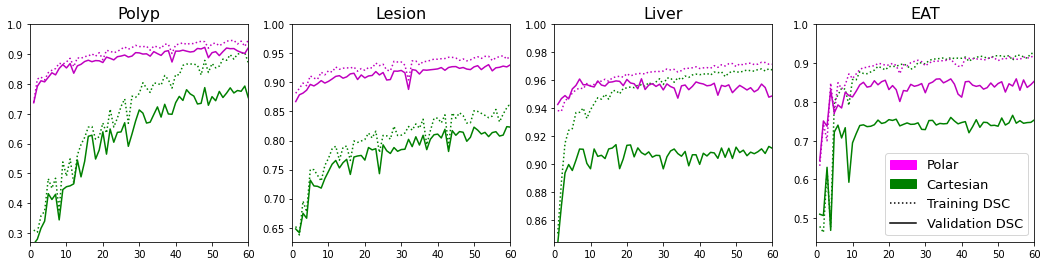
\includegraphics[width=\linewidth]{images/4/training-graphs}
		\caption{The training and validation Dice coefficient (DSC) of the polar and Cartesian U-Net models during training. \cite{bencevicTrainingPolarImage2021}}
		\label{fig:training}
	\end{figure}
	
\clearpage
		
We also train several models with both polar and Cartesian coordinates on subsets of the training dataset. Namely, we trained models on 25\%, 50\%, 75\%, and 100\% of the lesion training dataset for 50 epochs. The results of this training are shown in \figref{fig:dataset-vs-dsc}. The polar network is much more data efficient and achieves better results than the cartesian network even with only 25\% of the data.

	\begin{figure}[h]
		\centering
		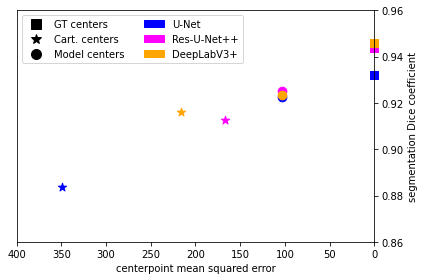
\includegraphics[width=0.65\linewidth]{images/4/mse-vs-dice}
		\caption{The relationship between mean squared errors of the centers used for the polar transformation and segmentation performance of the polar network on the lesion dataset. The mean squared errors are calculated compared to the ground-truth centers. \cite{bencevicTrainingPolarImage2021}}
		\label{fig:centers-vs-performance}
	\end{figure}

		\begin{figure}[h]
		\centering
		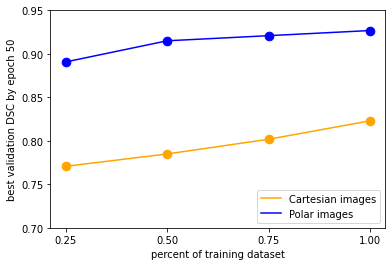
\includegraphics[width=0.65\linewidth]{images/4/dsc-vs-dataset-percent}
		\caption{The best Dice coefficient by epoch 50 for models trained on subsets of the lesion training dataset. \cite{bencevicTrainingPolarImage2021}}
		\label{fig:dataset-vs-dsc}
	\end{figure}
	
	\subsubsection{Discussion}
	
We obtain state-of-the-art results for polyp and lesion segmentation by training common biomedical image segmentation models. In the liver dataset, we achieve state-of-the-art results when compared to other 2D methods, but 3D methods 
achieve the same or slightly better results \cite{valanarasuKiUNetOvercompleteConvolutional2020a}. 
The liver dataset is 
by far the largest dataset we evaluated. As such, improvements gained from 
encoding localization information and reducing dimensionality might not be as large as in smaller 
datasets, since the network has enough data to learn these complex structures.
The EAT dataset is one where the task is not to find a single object, but instead, to segment multiple smaller 
pockets of tissue around the heart. This task is more challenging for common models like U-Net and 
requires a more complex approach \cite{zhangAutomaticEpicardialFat2020a}. It is possible that combining 
these existing approaches, namely segmenting the pericardium first, with training on polar coordinates 
would lead to an improvement in the state of the art.

	\begin{figure*}
	\subfloat[Polyp predictions]{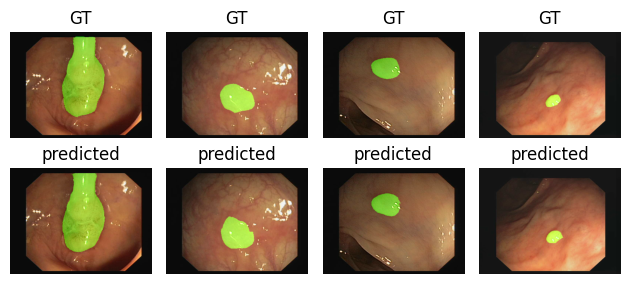
\includegraphics[width=0.49\columnwidth]{images/4/centerpoint_model_output_polyp}}
	\hfill
	\subfloat[Lesion predictions]{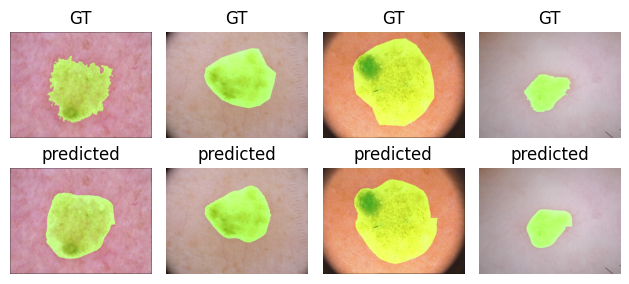
\includegraphics[width=0.49\columnwidth]{images/4/centerpoint_model_output_lesion}} \\
	\subfloat[Liver predictions]{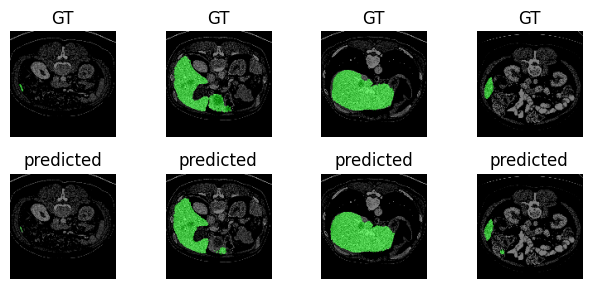
\includegraphics[width=0.49\columnwidth]{images/4/centerpoint_model_output_liver}}
	\hfill
	\subfloat[EAT predictions]{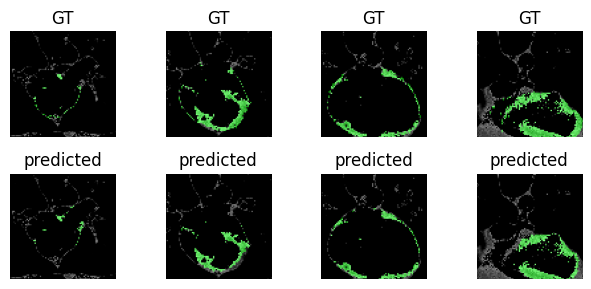
\includegraphics[width=0.49\columnwidth]{images/4/centerpoint_model_output_eat}} \\
	\caption{A random sampling of inverse polar transformed predictions from the polar network with the polar origins predicted from the centerpoint predictor for various datasets. The prediction is shown in green and overlaid on top of the original input image. EAT predictions (d) are cropped and zoomed to better show the predictions. \cite{bencevicTrainingPolarImage2021}}
	\label{fig:predictions}
	\end{figure*}

We also show that training on polar images leads to a significant improvement in segmentation performance 
when compared to training on Cartesian images for the same network architecture. Additionally, as shown in \figref{fig:training}, the polar 
network portions of our approach converge in much fewer epochs than the Cartesian networks. This is in part due to the location information being encoded in the image 
itself via the polar origin, and in part due to a possible data dimensionality reduction, allowing the 
network to more easily optimize the loss function. The polar networks are also more robust to low dataset 
sample size. This is especially important in biomedical image segmentation where the availability of large 
labeled datasets is often very limited.

Predicting the center point from the Cartesian model, while still an improvement over the plain 
Cartesian network leads to worse results than those obtained by the center point predictor model. 
We conclude that segmentation is highly dependent on choosing the correct polar origin. This 
dependency is somewhat loosened by adding polar origin augmentation when training the polar 
network.

	\begin{table}[t]
\centering
\def\arraystretch{1.2}
\begin{tabularx}{\linewidth}{X c c}
 Method & DSC & Difference \\ 
 \hline \\ [-2ex]
Cartesian & 0.8315 & - \\
Polar (Cartesian origins) & 0.8918  & +0.0603 \\
Polar (Centerpoint predictor) & 0.9094 & +0.0176  \\
 + centerpoint augmentation & 0.9288 & +0.0194 \\
 + polar network training augmentation & 0.9374 & +0.0086 \\ [1ex]
\end{tabularx}
\caption{Ablation study of our approach for the polyp dataset.}
\label{table:ablation}
\end{table}

\figref{fig:predictions} shows a random sampling of predictions from the polar network using the center point predictor for polar origins. Qualitatively, we conclude that the network achieves very good segmentation results, leading to a very high overlap with the target object. The network successfully segments both small and elliptical as well as large and unevenly shaped polyps. On the lesion images, the network predicts a smooth border when sometimes the actual border of the lesion is rough, as shown in the left-most example on \figref{fig:predictions}(b), however, the network still does a good job of delineating a lesion border even when the color of the lesion is very similar to the surrounding skin. The network successfully predicts a liver border both when the liver is very large and very small on the image, showing good scale invariance, but sometimes under segments the liver when multiple connected components are needed. On the EAT dataset, the network successfully learns to segment EAT despite its highly discontinuous and sparse distribution. However, the network sometimes under segments EAT.

Finally, we also perform an ablation study shown in \tabref{table:ablation}. Training on the polar coordinates with the polar origins predicted from the cartesian network yields the largest performance improvement. Predicting the polar origin from the center point predictor as well as adding center point augmentation to the predictor play a roughly equally important role in the performance. Lastly, a small performance improvement is further achieved by using data augmentation when training the polar network.

The center points could also be obtained by a more basic segmentation approach 
like thresholding or other traditional image processing methods, leading to a possible reduction in the 
number of required neural network parameters to achieve good segmentation. Furthermore, in our experiments,
we found that the segmentation is dependent on choosing the correct standard deviation of the generated 
heatmaps for training the center point predictor. An improvement to our method could be made by developing
a method to automatically estimate the standard deviation from the training or validation data without needing
to first train the center point predictor.

In conclusion, the polar transform demonstrates significant potential in simplifying the segmentation of elliptical objects, thus reducing the complexity of the neural network model required. However, a key limitation of this approach is that only one elliptical object can be segmented. The next section will introduce further advancements to this method, allowing the segmentation of multiple objects on the image.

\section{Supporting Multiple Transformations of an Image}

In this chapter, we've explored an approach where each image undergoes a single transformation before being processed by the segmentation network. We will now extend this model-driven preprocessing approach to accommodate multiple transformations of the same input image. This modification is particularly useful in scenarios where an image contains several objects, each with its distinct decision boundary. By applying a separate polar transformation for each object center, we can generate multiple segmentation maps for a single image. These maps can then be combined to create a unified segmentation result. The process involves the following steps:

\begin{enumerate}
	\item Our transformation predictor network will be enhanced to predict a set of transformation parameters \(\{\phi_1, \phi_2, \cdots, \phi_n\}\), where \(n\) varies based on the image and represents the number of transformations.
	\item For each transformation parameter in $\phi_i$ we will produce a corresponding set of transformed images $\{I'_i\}$, $I'_i = \mathcal{T}_{\phi_i}(I)$.
	\item Each transformed image $I'_i$ will be segmented using the segmentation network, producing a series of segmentation maps \(\{M_i\}\), where \(M_i = F_{seg}(I'_i)\).
	\item Finally, all of the segmentations will be fused using an aggregation function $f_{agg}$, resulting in a final segmentation map $M = f_{agg}(\{M_i\})$.
\end{enumerate}

To exemplify this, we will present a case of using the polar transformation as we did earlier, only this time we will be segmenting images with multiple connected components (objects) in their segmentation maps. Therefore, we will use multiple polar transformations for each image, one for each connected component. The transformation parameter predictor will be modified to predict the centroid of each connected component, instead of just a single centroid. Each centroid will be used to transform and segment the image. For the aggregation function, we will choose a weighted sum and a hysteresis thresholding function $th$ with thresholds $t_1$ and $t_2$:

\begin{equation}
	f_{agg}(\{M_i\}) = th(\sum_{i = 1}^n M_i W_i; t_1, t_2),
\end{equation}

each weight \(W_i\) functions as an image matching the dimensions of \(M_i\), where the pixels correspond to the relative importance of that pixel in the corresponding segmentation map. For instance, in the case of the polar transform, the value assigned to each element in \(W_i\) depends on its relation to the connected component associated with the polar origin for the corresponding segmentation mask \(M_i\). Specifically, elements that belong to the same connected component as the polar origin used for the \(i\)-th segmentation are assigned a value of 2. Elements outside this connected component are assigned a value of 1. With this weighing strategy, regions belonging to the connected component that is most beneficially transformed are more heavily weighted than other pixels.

The hysteresis thresholding function \(th\), defined by two thresholds \(t_1\) and \(t_2\), operates in two stages. Initially, it eliminates all pixels with intensity levels below \(t_1\). First, it removes all pixels with an intensity lower than $t_1$. Next, in the remaining pixels of the image, for each connected component, if any of the component's pixel intensities are higher than $t_2$, the whole connected component is preserved, otherwise the connected component is removed, as illustrated in \figref{fig:hysteresis-ccs}.

		\begin{figure}[h]
		\centering
		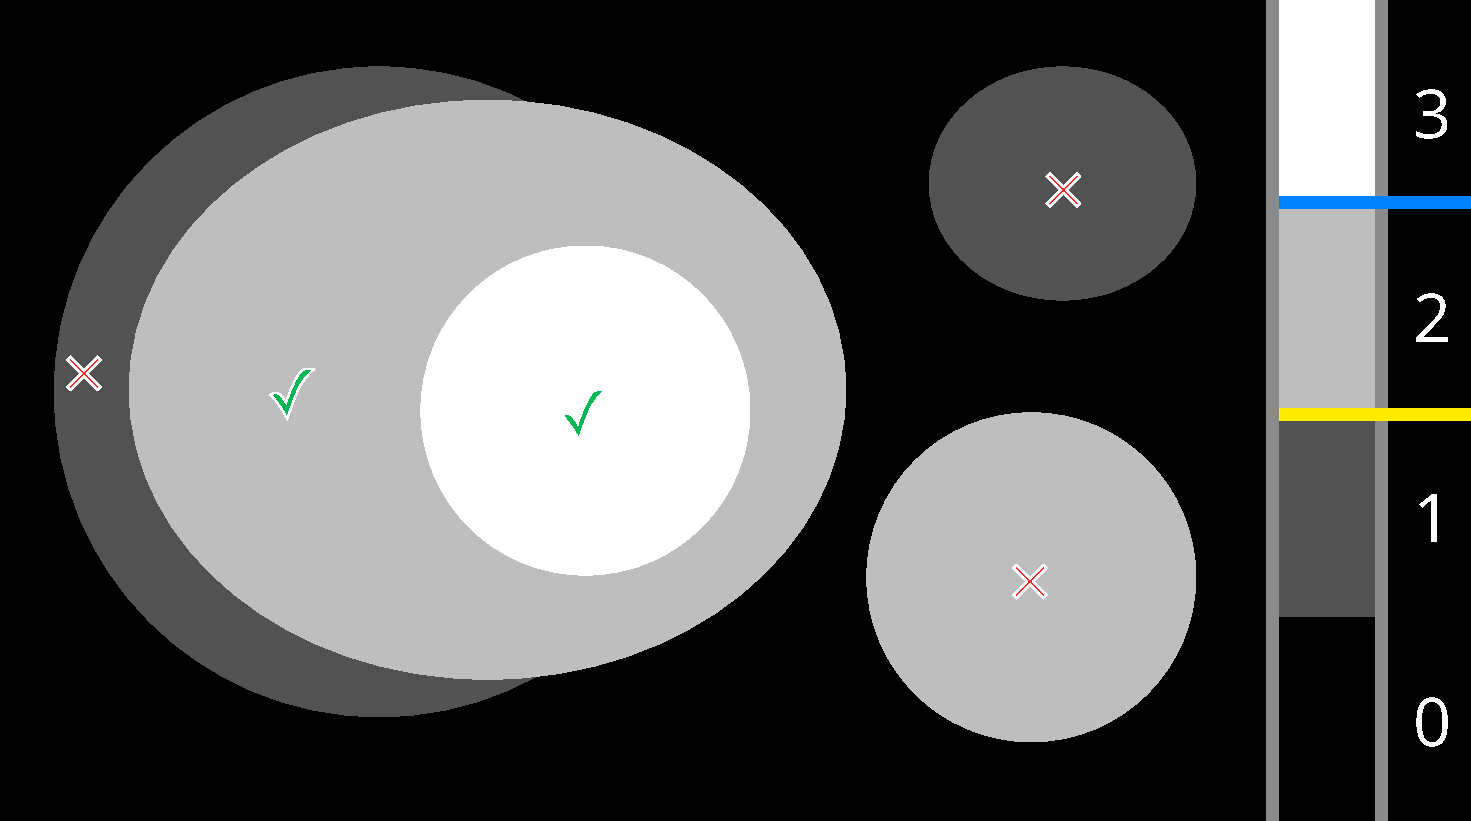
\includegraphics[width=0.7\linewidth]{images/4/hysteresis-ccs}
		\caption{A visual explanation of hysteresis thresholding. Kept regions are marked with green checkmarks, while deleted regions are marked with red crosses. The pixel intensity scale is shown on the right, where $t_1$ is marked in yellow and $t_2$ is marked in blue. All regions below $t_1$ are removed, while regions above $t_1$ are kept if they are connected to at least one pixel with intensity larger than $t_2$.}
		\label{fig:hysteresis-ccs}
	\end{figure}
	
The approach of model-driven preprocessing using multiple transformations has several advantages. First, each object can benefit from the reduction in segmentation complexity. For example, in the case of the polar transform, one object is always the bottom part of the polar transformed image to be segmented, so the network does not need to learn to first localize the object. Secondly, a consequence of this approach is that images with multiple connected components are over-sampled during training. This is beneficial since these images are usually under-represented (when compared to images with fewer connected components) and harder to segment (since they require segmenting multiple objects).
	
What follows is an empirical study of this approach for aorta segmentation, which is a modification of the one presented in \ref{polar-paper} to allow support for multiple transformations of the input image, one for each object in the image.

\section{Model-Driven Preprocessing using Multiple Transformations for Aorta Segmentation}

The aorta is the largest artery of the human body and supplies oxygenated blood from the heart to all parts of the body. It is one of the most clinically significant structures to analyze for cardiovascular disease diagnosis and prevention. Several conditions could occur on the aorta which can be detected using 3D medical imaging, including aneurysms, dissections, stenoses, coarctations, or traumas. All of these conditions can be dangerous and require careful screening, following, and potentially surgical treatment, while a failure or delay in the diagnosis of these conditions could be fatal. Therefore, developing a fully automated method to efficiently and accurately segment the aorta could be beneficial for earlier detection of these conditions. By producing a 3D model of the aorta from CT or MRI scans, a computer algorithm could perform automatic measurements to screen and detect aortic aneurysms, dissections, and other conditions that are commonly diagnosed by imaging the aorta.

Several methods based on deep learning were proposed for segmenting the aorta from CT images. \citet{fantazzini3DAutomaticSegmentation2020} use a cascade of U-Net-based networks. They first perform a rough segmentation on axial slices to extract a region of interest. They then use separate networks to segment axial, sagittal, and coronal slices of the region of interest. Several other papers have used 3D U-Net-based architectures for this task \cite{yuThreeDimensionalDeepConvolutional2021, chenMultistageLearningSegmentation2021}.

\subsection{Methodology}

The approach presented in this section is an extension of the approach presented in \ref{polar-paper}. We obtain the center points of the objects in the image using a rough segmentation from a U-Net-based network, instead of using a center point predictor as is described in \ref{polar-paper}. A summary of the approach is shown in \figref{fig:summary}.

\begin{figure}[h]
\centering
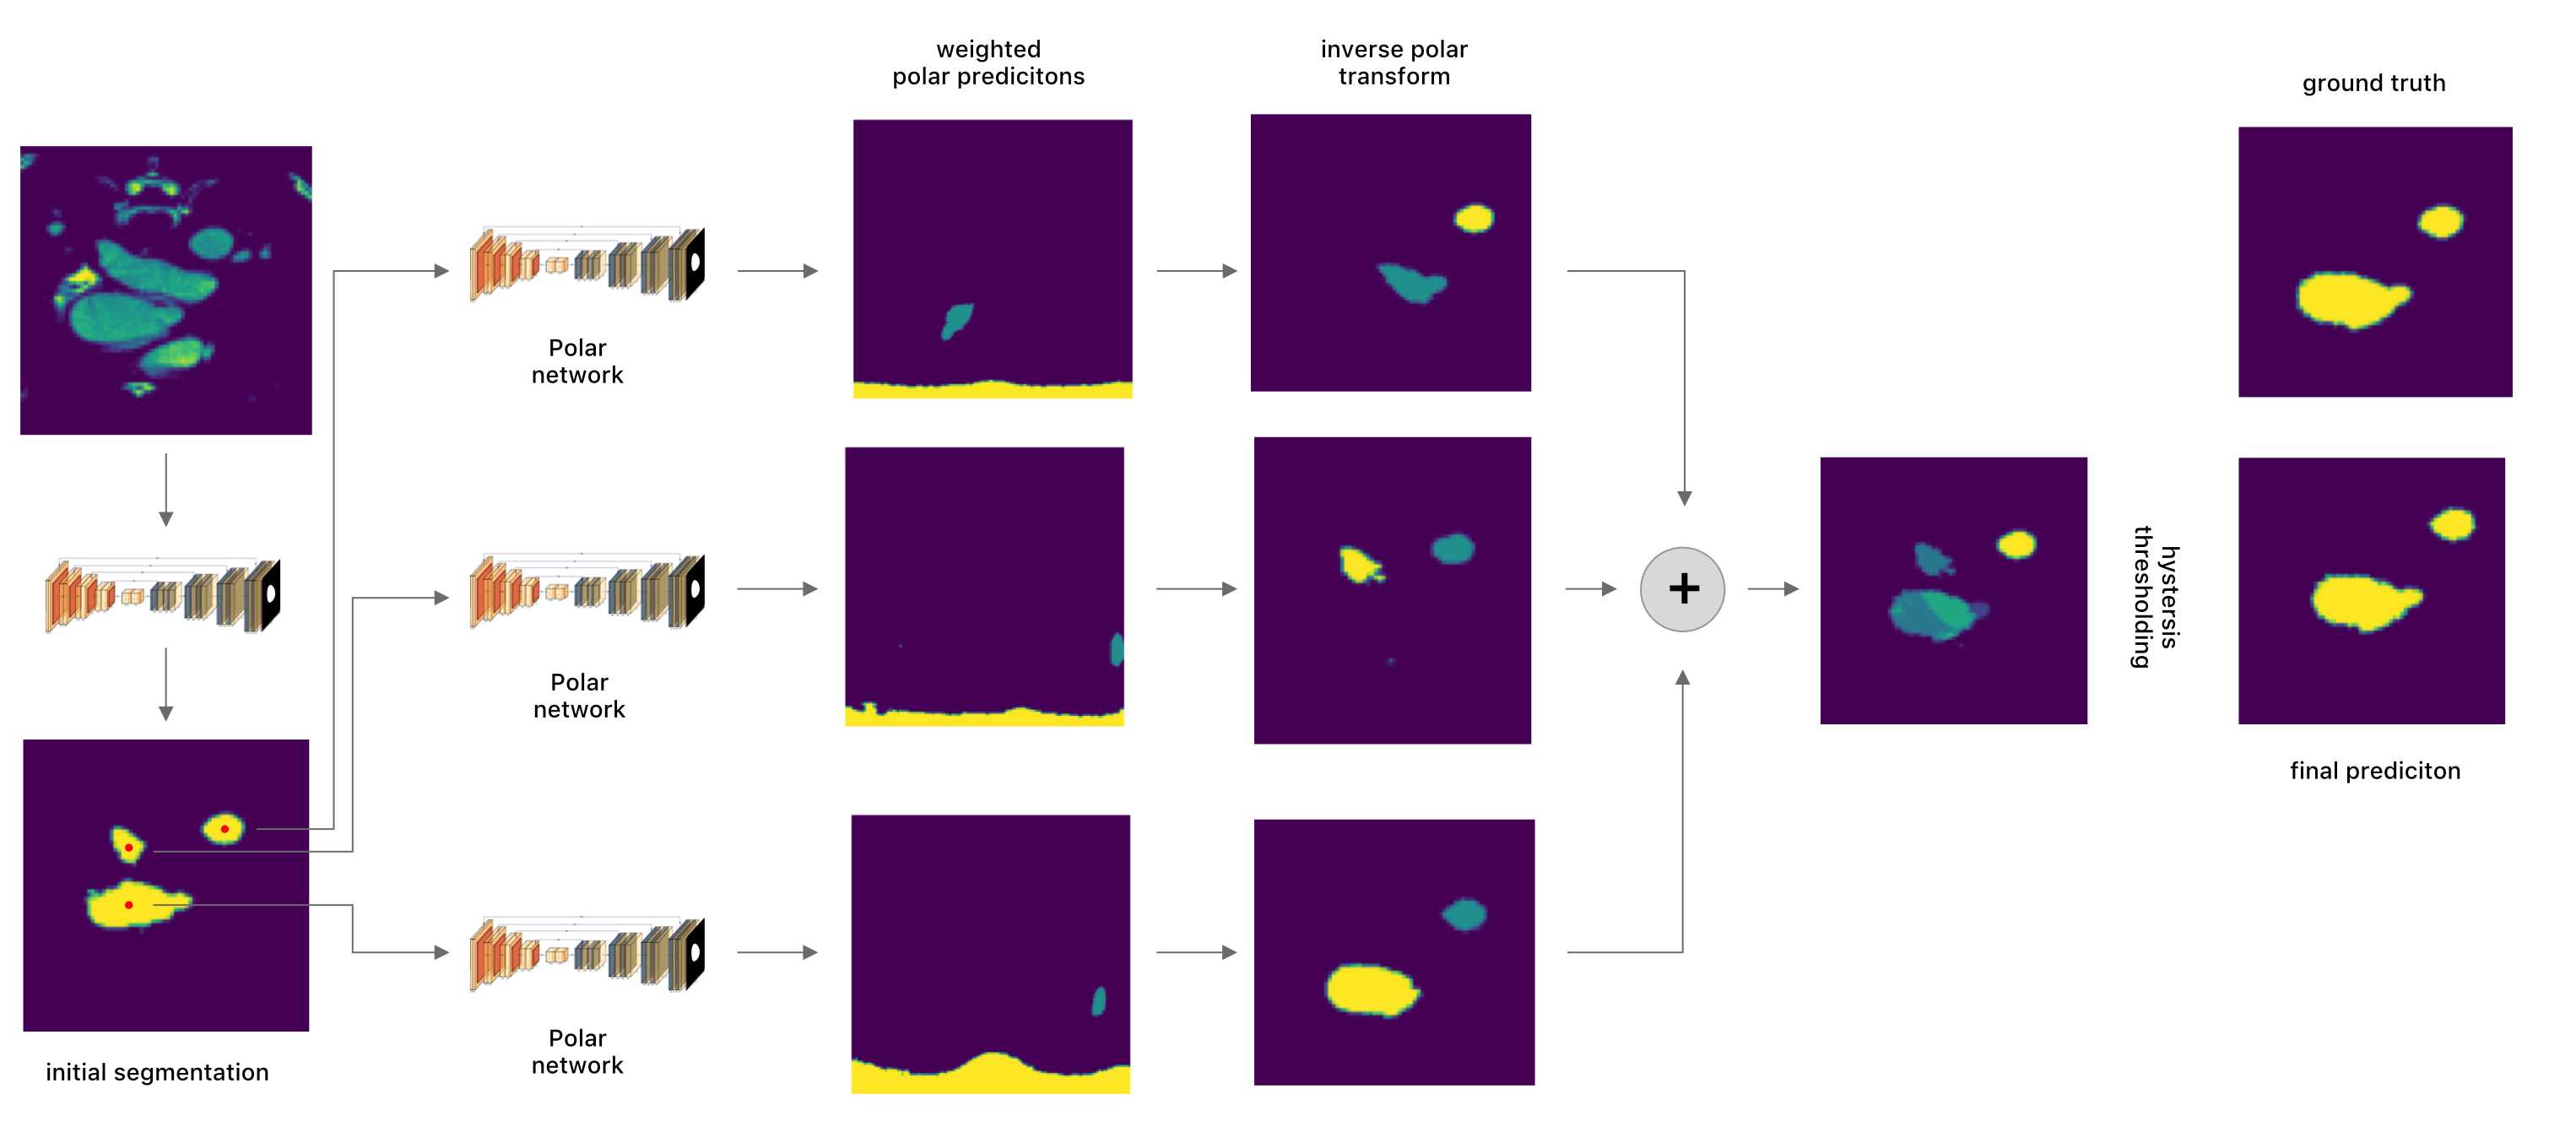
\includegraphics[width=\textwidth]{images/4/summary}
\caption{A summary of our approach. An input image is first segmented using a U-Net network. For each connected component in the segmentation, the input image is transformed to polar coordinates using the centroid of the connected component as the origin. These images are then fed into a U-Net trained on polar images, and the predictions for each object are fused, hysteresis thresholded, and transformed back to cartesian coordinates. Note how one of the false positive connected components in the initial segmentation was removed during hysteresis thresholding since the component was only predicted in one of the three polar predictions. \cite{bencevicUsingPolarTransform2022a}}
\label{fig:summary}
\end{figure}

As described earlier in this section, we perform several key modifications to allow the network to segment multiple objects on an image. During the training of the polar network, we construct a dataset that contains one polar transformation per connected component in the ground truth segmentation label. The origins of these polar transformations are the centroid of each corresponding connected component.

We also employ prediction fusion during inference. First, a 2D U-Net-based network is used to obtain an initial rough segmentation. A separate polar transformation for each connected component in the rough segmentation is constructed using the centroid of each component as the origin. The polar network predicts a segmentation map for each transform, resulting in a number of predictions equal to the number of connected components. In the predicted image, a weight of 2 is assigned to the connected component which contains the origin for that prediction, and a weight of 1 to all other connected components. We then sum all of the weighted images together. As shown earlier in this chapter, the polar network generally performs best on objects which contain the polar origin, and worse at predicting other objects on the image. Therefore, we assign a larger weight to that component as a proxy for a confidence measure. We then sum all of the weighted predictions together and normalize the prediction to a 0-1 range. This leads to a segmentation map where each non-zero pixel represents the confidence that the pixel belongs to the aorta class. To obtain the final segmentation, we use hysteresis thresholding where the bottom threshold is 0, and the top threshold is 0.4, empirically determined according to the best Dice coefficient on the validation dataset. An example of thresholding a prediction is shown in \figref{fig:thresh}.

\begin{figure}[h]
\centering
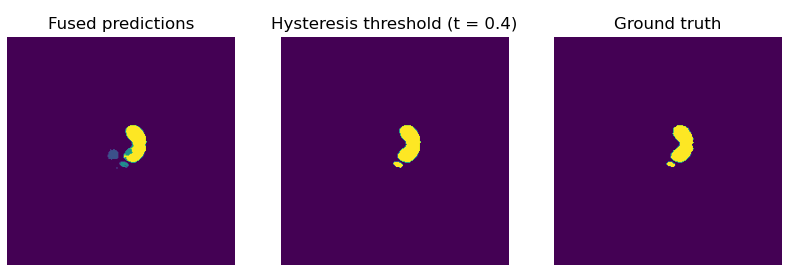
\includegraphics[width=0.8\columnwidth]{images/4/hyst}
\caption{Hystersis-thresholded segmentation output. For each polar prediction, the component that contains the origin of the transform gets a weight of 2 assigned, while all other components get a weight of 1. This left-most image is the result of summing the predictions of 3 polar transformations of the original image (one for each connected component), converted to cartesian coordinates. Note how the thresholding removes the false positive object on the left of the image while keeping the true positive objects intact. \cite{bencevicUsingPolarTransform2022a}}
\label{fig:thresh}
\end{figure}

\subsubsection{Data Description and Preprocessing}

We used a publicly available dataset of CT scans with corresponding aorta labels \cite{radlAVTMulticenterAortic2022} including the ascending aorta, the aortic arch as well as the descending and abdominal aorta. While the original dataset contains scans from three different centers, in our experiments, we only use the data from Dongyang Hospital. In total, we use 18 CT scans, each containing 122-251 slices, with a slice thickness of 2 or 3 mm.

Each CT slice is windowed to a range of 200 to 500 HU to remove information from irrelevant tissues, then normalized to a range of -0.5 to 0.5, and zero centered using the global mean value across all slices in the validation set. The slices were each resized from $512 \times 666$ to $256 \times 256$ pixels. We use augmentation during training for both the cartesian and the polar network. The augmentations we use include a $50\%$ chance of a random combination of affine transforms including a shift of up to $6.25\%$, a scale of up to $10\%$ and a rotation of up to $15^{\circ}$; as well as a $30\%$ chance of a horizontal flip.

All of our models were implemented using PyTorch 3.9 using an NVIDIA GeForce RTX 3080 GPU. We use the U-Net \cite{ronnebergerUNetConvolutionalNetworks2015d} architecture for both the cartesian and the polar network. For training, we use a batch size of 8 and the Adam optimizer with a learning rate of $0.001$. All models were trained for 60 epochs with checkpointing where the model with the best validation Dice coefficient was selected. We use the Dice loss function as described in the previous section of this chapter. All of the code, as well as the trained networks, can be found at \href{https://github.com/marinbenc/medical-polar-training}{github.com/marinbenc/medical-polar-training}.

\subsection{Results and Discussion}

\begin{table}[h]
\def\arraystretch{1.2}
\centering
\begin{tabularx}{\linewidth}{X c c c c} 
 \textbf{Method} & \textbf{DSC} & \textbf{mIoU} & \textbf{Prec.} & \textbf{Rec.} \\ 
 \hline
U-Net (non-polar) & $0.886 \pm 0.049$ & $0.825 \pm 0.052$ & $0.901 \pm 0.074$ & $0.893 \pm 0.039$ \\
Polar + GT centers & $0.937 \pm 0.053$ & $0.895 \pm 0.055$ & $0.944 \pm 0.064$ & $0.937 \pm 0.040$ \\
Polar + NP centers* & $0.932 \pm 0.027$ & $0.895 \pm 0.033$ & $0.915 \pm 0.040$ & $0.973 \pm 0.018$ \\
\end{tabularx}
\caption{A summary of the mean segmentation results of our experiments. \textit{Non-polar} are the results of the U-Net trained using cartesian images. \textit{Polar + GT centers} are the results of the U-Net trained on polar images, using ground-truth connected component centers during inference, as an example of the best case possible results. \textit{Polar + NP centers} are the results when running inference on the polar model using center points obtained from the non-polar model predictions. *Our proposed method.}
\label{table:results}
\end{table}

To perform evaluation, we use 3-fold cross-validation on the 18 scans. For each fold, we train a polar and non-polar model using the slices of 12 CT scans and run inference on the slices of the remaining 6 scans. All results presented in this section are averaged across each CT scan and then across the three folds.

\begin{figure}[h!]
\centering
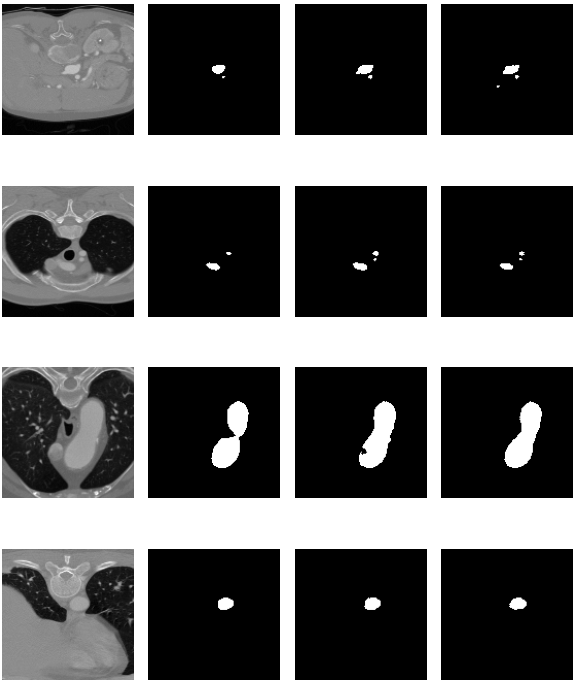
\includegraphics[width=\columnwidth]{images/4/examples_3}
\caption{Random examples of predictions. Columns from left to right show: the input image, the initial prediction from the non-polar network, the final fused polar prediction, and the ground truth segmentation label. \cite{bencevicUsingPolarTransform2022a}}
\label{fig:examples}
\end{figure}

A summary of our segmentation results is presented in \tabref{table:results}. Random examples of segmentation results are shown in \figref{fig:examples}. In the experiments in \ref{polar-paper} the polar networks achieve the best segmentation performance when using accurate center points during inference. As the accuracy of the center points goes down, so does the segmentation performance. The experiments in this paper follow the same pattern, the polar networks perform significantly better than the cartesian networks when using ground truth centers. However, even with less accurate centers obtained from initial rough segmentation by the non-polar network, the results yield only slightly lower Dice coefficients than when using ground-truth centers directly. The non-polar network can also be seen as a baseline model, and our approach results in a significant improvement over this baseline in all segmentation metrics.

In some problems in medical imaging, e.g. segmenting cancerous tissues, a higher recall is beneficial since the cost of missing tissues can be very high \cite{tahaMetricsEvaluating3D2015}. A key advantage of our approach is that by fusing multiple predictions and using hysteresis thresholding the threshold value can be used to impact the precision--recall tradeoff. Our experiments show that the average per-patient pixel-level recall increased when compared to the baseline model.

We also present the standard deviation across CT scans as a measure of segmentation reliability. Using the polar coordinates decreases the standard deviation between patients of all performance metrics, indicating that the predictions are more reliable and more robust to inter-patient differences. To further emphasize this, we present a box plot of segmentation results for each patient in \figref{fig:box}. Note that, in contrast with the baseline model, when using our approach there are no outliers in the box plot.

\begin{figure}[h]
\centering
\includegraphics[width=0.7\columnwidth]{images/4/box_plot}
\caption{A box plot of the per-scan Dice coefficients of our experiments. \textit{Non-polar} are the results of the U-Net trained using cartesian images. \textit{Polar + GT centers} are the results of the U-Net trained on polar images, using ground-truth connected component centers during inference. \textit{Polar + NP centers} are the results when running inference on the polar model using center points obtained from the non-polar model predictions. \cite{bencevicUsingPolarTransform2022a}}
\label{fig:box}
\end{figure}

A comparison of our results with other deep learning-based approaches for aorta segmentation in the literature is shown in \tabref{table:comparison}. Our approach achieves performance comparable to the state of the art, and a large improvement over the baseline methods. Note that the results are evaluated on different datasets and with a different number of cases. Therefore, it is hard to objectively compare these approaches.

\begin{table}[h]
\def\arraystretch{1.25}
\centering
\begin{tabularx}{\textwidth}{X l l c}
 \textbf{Method} & \textbf{DSC} & \textbf{mIoU} & \textbf{n}\\ 
 \hline
\citet{yuThreeDimensionalDeepConvolutional2021} & 0.958 & - & 25 \\
\citet{fantazzini3DAutomaticSegmentation2020} & $0.928 \pm 0.013$ & $0.866 \pm 0.023$ & 10 \\
\citet{cheungComputationallyEfficientApproach2021} & $0.912$ & - & 14 \\
Proposed method & $0.932 \pm 0.027$ & $0.895 \pm 0.033$ & 18 \\
\end{tabularx}
\caption{A comparison of our approach with results reported in papers describing deep learning-based aorta segmentation methods. Note that the datasets used for obtaining the results are not the same. $n$ is the number of cases used to obtain the evaluation.}
\label{table:comparison}
\end{table}

% END AORTA PAPER

  \section{Conclusion}
    
In this chapter, we've outlined an approach to enhance data efficiency in medical image segmentation by employing two smaller neural networks, rather than a single large one. The first network is designed to predict parameters for a strategically chosen transformation, aimed at reducing the complexity of segmentation. The second network then handles the segmentation of these transformed images. Our empirical studies, particularly with the polar transform, demonstrate the efficacy of this approach across various medical imaging segmentation tasks. We observed notable improvements in training efficiency, especially in cases involving the segmentation of a single, roughly elliptical object. Furthermore, segmentation of polar-transformed images has shown state-of-the-art results in small datasets and near state-of-the-art performance in larger datasets, even when utilizing generic, low-parameter-count models such as U-Net.

We've enhanced this approach by introducing the capability to perform multiple transformations on a single image, followed by the fusion of segmentation results from each transformation using hysteresis thresholding. Applying this method using polar transformations of CT images of the aorta improved segmentation results compared to baseline networks trained on Cartesian images. This improvement was observed across various metrics without a substantial increase in training time or network architecture complexity. Moreover, the fusion of individual object segmentations on an image through hysteresis thresholding has proven beneficial in increasing pixel-level recall, a valuable trait in medical image segmentation tasks.

We have further improved this approach by allowing multiple transformations of the same image and fusing segmentations of each transformation using hysteresis thresholding. When applied to the polar transform, we showed that this leads to large improvements over baseline networks trained on cartesian images for segmenting the aorta. We see improvements across a variety of metrics without significantly increasing training times or the complexity of the used neural network architectures. In addition, by fusing separate predictions of different objects on the image with hysteresis thresholding we can increase pixel-level recall (at the cost of accuracy) which is often beneficial in medical image segmentation tasks. 

This is a flexible approach that allows leveraging domain knowledge as it can be used with any invertible image transformation. Moreover, it is invariant to the downstream segmentation architecture as it is a separate network. Thus, it can be used as a general preprocessing step regardless of the segmentation method. Moreover, if the transformation parameter predictor and segmentation networks share similar architectures, one can use transfer learning between the two networks. The approaches presented in this chapter have been published in \cite{bencevicTrainingPolarImage2021} and \cite{bencevicUsingPolarTransform2022a}.

\printbibliography[heading=subbibintoc]
\end{refsection}

\begin{refsection}
% Kapitel 3

\chapter{Reducing Model Input Sizes with Model-Driven Crops}
\label{chap:reducing-input-size}

In Chapter \ref{chap:data-efficiency} of this thesis we discussed how increasing the number of parameters of a model allows it to overfit more easily. Additionally, we discussed how more complex problems require more parameters to be modeled. Thus, for small datasets, it is beneficial to reduce the complexity of the problem to allow for using networks of fewer parameters. A simple way to reduce the complexity of problems in convolutional neural networks is to reduce the size of the images.

To understand how reducing input size reduces model complexity, let's revisit the concept of sample complexity \(n(\epsilon, \delta)\) and its established bounds:

\begin{equation}
	n(\epsilon, \delta) \geq \frac{\log(\lvert \mathcal{F} \rvert / \delta)}{\epsilon},
\end{equation}

Here, \(n\) represents the minimum number of samples needed for a model from the hypothesis space \(\mathcal{F}\) to achieve a performance that is 'probably approximately correct'—that is, within an error margin \(\epsilon\) with a confidence level of \(1 - \delta\). It's clear from this relation that as the size of the hypothesis space expands, so does the sample complexity.

The hypothesis space refers to the set of all functions that the model is capable of approximating, encompassing every conceivable mapping from the domain \(\mathcal{D}\) to the codomain \(\mathcal{C}\). Therefore, the magnitude of the hypothesis space can be expressed as:

\begin{equation}
	\lvert \mathcal{F} \rvert = {\lvert C \rvert}^{\lvert D \rvert}.
\end{equation}

For binary CNN-based image segmentation, the model maps \(c\)-channeled images \(I \in \mathbb{R}^{w \times h \times c}\) to binary masks \(M \in \{0, 1\}^{w \times h}\). The hypothesis space thus grows with the image dimensions \(w, h\), and the number of channels \(c\). Reducing image size directly decreases the hypothesis space, lowering the sample size needed for effective training. This relationship is supported by empirical findings --- \citet{tanEfficientNetRethinkingModel2020} show that convolutional neural networks perform best when input size, network depth, and width are scaled proportionally.

Smaller input sizes also offer technical benefits, notably reduced memory demands. Since CNN memory requirements grow exponentially with image size, larger inputs significantly limit batch size during training. This constraint not only slows down the training process but can also affect the accuracy of gradient estimates per batch, potentially destabilizing training.

The method of image scaling is crucial for performance in medical image segmentation tasks, where images are typically downscaled uniformly. This process can lead to the loss of critical fine details, such as edges, which are vital for segmentation accuracy in medical imaging. For example, the pericardium's thin structure around the heart, often less than 2 mm and represented by only a few pixels in cardiac CT scans, can be obscured or entirely lost through downsampling. This information loss is particularly detrimental for small objects, which are prevalent in medical images.

An effective way to overcome this loss of information while still reducing the image is cropping the image to a region of interest. By focusing on the area containing the target object for segmentation, the network's learning task is simplified, removing the need to filter out irrelevant background areas. Additionally, centering and uniformly scaling the object across images can further reduce the variance of the data, enabling the network to use fewer parameters. Given this, we will now propose a method to effectively use image cropping as a way of reducing neural network input size.

\section{Model-Driven Image Cropping}

We introduce a strategy to minimize the input size for segmentation networks, focusing on cropping rather than uniform downsampling. This method involves isolating each object within the original high-resolution image, cropping these areas, and performing segmentation on the individual cropped sections. By concentrating on smaller crop regions instead of the entire image, we significantly reduce the network's input size while preserving essential pixel information within the objects. This approach is illustrated in \figref{fig:summary}, providing a visual summary of the process.

\begin{figure}[H]
\centering
\includegraphics[width=\textwidth]{images/5/explainer-diagram.png}
\caption{A visual summary of our approach. (1) An image is uniformly downsampled from its original resolution. (2) A rough segmentation is predicted by a neural network, and the bounding box of each connected component is calculated. (3) The bounding boxes are scaled to the original image space and crops of the input image are taken in the original resolution and scaled to a common input size. (4) Each crop is segmented separately by a second neural network specifically trained on cropped images. These crops are fused to form a final segmentation in the original high resolution. \cite{bencevicSegmentthenSegmentContextPreservingCropBased2023a}\label{fig:summary}}
\end{figure}

The inference procedure using our method is as follows. Let $I$ be an input image of size $W \times H$. We obtain a rough segmentation using $M_{rough} = g_{\phi_1}(C(I))$, where $M_{rough}$ is a binary segmentation mask generated by $g_{\phi_1}$, a CNN with input and output size $S \times S$, parameterized by $\phi_1$; and $C$ is a uniform downsampling operation from  $W \times H$ to $S \times S$. 

Given $N$ connected components of $M_{rough}$, a set of bounding boxes $\{b_i\}, i \in [1..N]$ is calculated enclosing each connected component, described in more detail later in this chapter. The bounding boxes are used to generate a set of crops $\{I_i: I_i = I(T_i(b_i))\}$, where $T_i$ is a scaling and translation of the bounding box in $S \times S$ space to the corresponding region in the $W \times H$ space.
The crops are used to generate a set of fine segmentation masks $Y_f$ using:

\begin{equation}
Y_f = \{Y_{fi}: Y_{fi} = g_{\phi_2}(C_i(I_i)), i \in 1..N\},
\end{equation}

where $g_{\phi_2}$ is a CNN of the same architecture as $g_{\phi_1}$ and size $S \times S$, parameterized by $\phi_2$, and $C_i$ is a scaling operation from the width and height of $I_i$ to $S \times S$. A final segmentation $y$ is formed using:

\begin{equation}
y = max(\{(T_i \circ C^{-1}_i)(Y_{fi}), i \in 1..N\}),
\end{equation}

where $y$ is the resulting segmentation formed as the maximum value in all of the fine segmentations, transformed to their corresponding regions in $W \times H$ space. This process is described in more detail in Algorithm \ref{alg:crop}. 

The rough segmentation network $g_{\phi_1}$ is trained on uniformly downsampled images. The network outputs a rough, low-resolution segmentation mask. The rough segmentation mask contains a number of connected components. For each connected component, we calculate a bounding box that encompasses all of its pixels. These bounding boxes are the crop regions used for the fine segmentation network. Since we only use this segmentation to obtain rough regions of interest, the input images to this network can be heavily downsampled without impacting the final fine segmentation.

The fine segmentation network $g_{\phi_2}$ is trained on cropped images using the ground truth segmentation masks to generate the bounding boxes. This network produces a fine segmentation of that region of the image. Since we know the original bounding box of each crop, we can resize the final segmentation to its original size and translate it to its original position. We perform this for each object in the image, fusing each of the fine segmentation masks into a final segmentation mask in the original image resolution.

In other words, our method performs zooming and panning around the original image and builds a final segmentation piece-wise from each zoom and pan. This allows us to use neural networks with very low input sizes without requiring a large amount of downscaling. What follows is a detailed description of the different parts of the segmentation process.

\begin{algorithm}
\caption{Inference algorithm for one input image}\label{alg:crop}
\begin{algorithmic}
 \renewcommand{\algorithmicrequire}{\textbf{Input:}}
 \renewcommand{\algorithmicensure}{\textbf{Output:}}
\Require High-resolution input image $I$ of size $H \times W$, \\
         input size $S$, padding $k$, \\
		 neural network NET\_1 trained in $S \times S$ downscaled images, \\
		 neural network NET\_2 trained on ground truth $S \times S$ image crops.
\Ensure Output image $Y$ of size $H \times W$.
\\
\State $I' \gets \Call{resize}{I, (S, S)}$
\State $y' \gets \Call{net\_1}{I'}$
\State $y' \gets \Call{resize}{y', (H, W)$}
\State $ccs \gets \Call{connected\_components}{y'}$
\State $crops \gets [ ]$ \Comment{An array of $S \times S$ images}
\State $bboxes \gets [ ]$ \Comment{An array of bounding boxes for each crop}
\\
\For{cc in ccs}
	\State $bbox \gets bounding\_box(cc)$
	\State $bbox.width \gets bbox.height \gets \Call{max}{bbox.width, bbox.height}$
	\State $bbox \gets (bbox.left - k, bbox.top - k, bbox.width + k, bbox.height + k)$
	\State $bbox \gets \Call{shift\_to\_image\_region}{bbox, (H, W)}$
	\State $crops.\Call{add}{\textsc{crop}(I, bbox)}$
	\State $bboxes.\Call{add}{bbox}$
\EndFor
\\
\For{crop, i in crops}
	\State $l, t, w, h \gets bboxes[i]$
	\State $crop \gets \Call{resize}{crop, (S, S)}$
	\State $y_{crop} \gets \Call{net\_2}{crop}$
	\State $y_{crop} \gets \Call{resize}{y_{crop}, (h, w)}$
	\State $Y[t:t+h, l:l+w] \gets Y[t:t+h, l:l+w]\ ||\ y_{crop}$
\EndFor
\end{algorithmic}
\end{algorithm}

\subsubsection{Cropping}\label{cropping}

The key to reducing downscaling in our approach is that we take crops from the image in the original resolution. The crop regions themselves are predicted on a downscaled image and then projected to the original image space.

The cropping procedure is as follows. First, a bounding box fully encompassing each connected component in the rough segmentation is calculated. The coordinates of the bounding box are then scaled to the high-resolution image space. An empirically determined padding of $S/8$ (for an $S \times S$ input size) is added along each of the four sides. This way of cropping preserves the context of the object and decreases the number of false negatives inside the bounding box.

The box is then squared, i.e. its height and width are set to the larger of the two dimensions. The box is also shifted (maintaining its width and height) to be fully inside the region of the image. Finally, the bounding box is used as a region to crop the original high-resolution image. The rough segmentation sometimes results in noisy regions, so each crop whose width or height is less than 5 pixels is discarded.

\pagebreak

\subsubsection{Fine Segmentation and Fusion}

Each crop of the high-resolution image is scaled to the input size of the fine segmentation network. The fine segmentation network outputs a number of segmentation masks equal to the number of connected components in the rough segmentation. A high-resolution segmentation mask is created by translating and scaling each of the fine segmentation network outputs to their original position. By doing so we construct a full segmentation piece by piece, where each piece is a fine segmentation of a single object in the image, as detected by the rough segmentation. If the cropped regions overlap in the final segmentation, we use a logical \verb|OR| operator to resolve the conflict in the fine segmentation mask. This process is presented in Algorithm \ref{alg:crop}.

\subsubsection{Training the Fine Segmentation Network}

The fine segmentation network is trained on ground truth image crops. The crops are obtained by using the connected components of ground truth segmentation masks. From there, the crops are prepared in the same way as described above. Since the images have multiple crop regions, we choose one of the crop regions of the full-resolution image at random during each training iteration. If the original image has no connected components in the ground truth segmentation mask, the whole image is used as training input. All input images to the fine segmentation network are resized to $S \times S$, where $S$ is a pre-determined input size that matches the input size used to train the rough segmentation network.

During training, we add an augmentation step in the form of crop region jittering. When preparing the crops during training, a uniformly distributed random number between $\pm16$ pixels is added to each dimension of the bounding box (the $x$- and $y$-coordinate, width, and height). This ensures that the trained network is robust to imperfect rough segmentation masks during inference.

In our experiments, we used the same architecture for both the rough and fine segmentation networks, as this allows us to use transfer learning. However, there is no requirement that the networks use the same architecture.

\subsection{Related work}

The approach presented in this chapter is motivated partly by the work of \citet{Qiu2018}, where a dataset of images is manually cropped to the object boundary, leading to an increase in segmentation performance. This was applied to skin lesions where it achieved a scale-unifying effect across the dataset. In this chapter, we adapt this approach to use a neural network to predict the optimal object boundary and develop specific ways to train the fine segmentation network on cropped images. In addition, we allow for taking multiple crops on the image and later fusing them in the final segmentation, which makes the method applicable to a wider range of segmentation tasks.

 In the previous chapter, a related approach is presented using the polar transform as a pre-processing step. The main novelty in this chapter is the use of cropping as a transformation step. The rest of the approach was then adapted to better suit a cropping transformation, including bounding box augmentation and padding the bounding box. This allows our approach to be used to reduce the input size of the networks.
 
\subsubsection{Detect-then-segment}

Several recent end-to-end neural network architectures for segmentation incorporate cropping in one of their layers \cite{girshickRichFeatureHierarchies2014, heMaskRCNN2017}. These generally use object detection to find a region of interest which is then segmented. This approach can be called \textit{detect-then-segment}. In models such as R-CNN \cite{girshickRichFeatureHierarchies2014} the objects are first detected and then fed into the segmentation pipeline. Mask R-CNN \cite{heMaskRCNN2017} uses object detection to extract a region of interest in the feature masks within the network. These methods effectively concentrate the network on a region of the image. However, information is still lost if the images are uniformly downsampled as a preprocessing step. In contrast, our approach allows one to use low input sizes by cropping the image before it enters the network. Compared to \textit{detect-then-segment} approaches, cropping as a preprocessing step reduces the number of parameters while increasing the pixel-level information in the salient regions of the image. In addition, our approach leads to rescaling each object to the same size before the fine segmentation, which increases the scale-invariance of the models.

\subsubsection{Coarse-to-fine Segmentation}

Our approach can be described as a coarse-to-fine approach to image segmentation. There have been similar approaches to medical image segmentation. \citet{zhouFixedPointModelPancreas2017} describe an approach to pancreas segmentation using a fixed-point model \cite{pmlr-v28-li13b}. They train a coarse and a fine segmentation network. The coarse network obtains an initial region of the pancreas which is then re-segmented using the fine network. The fine network then re-segments its output again, and this process is repeated iteratively until a stable solution emerges. They also use bounding box augmentation during training. Our approach differs in two ways. Firstly, we only use one iteration at a stable input size, improving the inference time. Secondly, our approach supports segmenting multiple objects on the image.

\citet{zhu3DCoarsetoFineFramework2018} describe an approach to pancreas segmentation with two neural networks. The first network is a coarse segmentation network trained on overlapping 3D regions of the whole CT volume. The second network is a fine segmentation network that is trained on only the regions where the ground-truth images contain the pancreas. During inference, the fine network re-segments densely overlapping regions of the rough segmentation. The main difference in our approach is the use of only one region of interest per object where the whole object is visible and uniform in scale. This allows us to use networks of a lower capacity while still maintaining good segmentation results.

Similarly to our approach, \citet{jhaInstanceSegmentationWhole2021} split the segmentation process into detection and segmentation stages. They use a neural network to first detect an object in a downsampled image. They then use the bounding box to crop the object in the high-resolution image. Our approach differs in several ways. Firstly, our approach allows the detection of multiple objects on the image and describes a way to fuse the segmentations of different objects. Secondly, we present new ways to train the fine segmentation network to make the fine segmentation network more robust to imperfect bounding boxes. Finally, we propose a generalized approach evaluated on a variety of different modalities of medical images.

\subsubsection{Non-uniform Downsampling}

The resolution of an input image for neural networks can be reduced using a more complex sampling strategy. \citet{marinEfficientSegmentationLearning2019} use non-uniform downsampling for this task. Their approach consists of training a neural network to sample points near object boundaries. The sampling points are then used to downsample the image and perform a final segmentation using a second neural network trained on the downsampled images. Similarly, \citet{jin2022learning} use a learnable deformable downsampling module which is trained together with a segmentation module end-to-end. Our approach differs in the use of cropping instead of non-uniform downsampling, which preserves the topology of the image and provides localization of the object.

\subsubsection{Other Approaches to Reducing Input Resolution}

Recently, transformer-based architectures such as SegFormer \cite{xie2021segformer} and the Swin Transformer \cite{liu2021Swin} have become popular approaches to semantic segmentation. These networks are trained on a large number of small, overlapping patches of the image. The network uses self-attention to determine the saliency of each patch. In a sense, this allows the network to be trained on very small input image dimensions. However, transformers require a very large amount of data to be trained and have large memory requirements \cite{dosovitskiy2020vit}, so their use is currently limited in the domain of training on downscaled medical images.

For whole slide images, the input size is often reduced by dividing the image into equally sized patches \cite{nazeriTwoStageConvolutionalNeural2018, houPatchBasedConvolutionalNeural2016}. A downside of this approach is computational complexity during inference since not all patches are relevant. Additionally, errors can arise when the objects are split by the patch boundary.

%%%%%%%%%%%%%%%%%%%%%%%%%%%%%%%%%%%%%%%%%%
\subsection{Results}

We evaluate our approach on three separate datasets, hereafter referred to as the cells, aorta, and polyp datasets. First, for each dataset, we trained a rough segmentation U-Net, Res-U-Net++, and DeepLabv3+ network at various downscaled input resolutions. These models are also used as baseline models to compare against our approach. To evaluate our approach, we train fine segmentation models using the same combinations of datasets, architectures, and input sizes. 

Altogether more than 100 neural networks were trained to evaluate our approach, including both the baseline networks and networks trained on cropped images.

Each network is trained from scratch using the downscaled dataset. The outputs from the networks are then upscaled to the datasets' original resolution, and the metrics are calculated using those outputs. We use the held-out test datasets for all of the results reported in this section. The baseline models are used as the rough segmentation networks for the experiments using our approach. The hyperparameters used for each network are reported in Table \ref{tab:hyperparams}.

In the interest of providing objective metrics of model performance, all of the hyperparameters were tuned using the validation dataset on the baseline U-Net. Those same hyperparameters are then used for each of the models in our approach. Each model is trained using the Adam optimizer up to a maximum number of epochs and the best model with the best validation loss is saved during training. The validation loss is calculated as the Dice score coefficient (DSC) over the validation dataset at the same resolution as the input images. We do not upscale the outputs for the validation loss as we do for calculating the final metrics. Each model was trained using PyTorch 1.10 on an Nvidia GeForce RTX 3080 GPU. Where possible, we have fixed the random seed value to ``2022'', but we have also run the experiments on two other random seeds and obtained similar results.

\begin{table}[H]
\caption{The hyper-parameters used for each of the models in our experiments.\label{tab:hyperparams}}
\newcolumntype{C}{>{\centering\arraybackslash}X}
\begin{tabularx}{\textwidth}{CCCC}
\textbf{Dataset} & \textbf{Batch size} & \textbf{Learning rate} & \textbf{Max. epochs} \\
\midrule
Cells & 16 & $5 \cdot 10^{-4}$ & 100\\
Polyp & 8 & $10^{-3}$ & 175\\
Aorta & 8 & $10^{-3}$ & 100\\
\end{tabularx}
\end{table}
\unskip

\subsubsection{Datasets}\label{datasets}

This section briefly describes the datasets used in our experiments as well as the preprocessing steps for the images. For more details, we direct readers to the supplemental code repository available at \href{https://github.com/marinbenc/segment-then-segment}{github.com/marinbenc/segment-then-segment}. To evaluate our approach, we chose three datasets across different medical imaging modalities, including CT scans, microscopy imaging, and colonoscopy images. We hope that the variety in the datasets will show the generalizability of our approach. Aside from the variety, the datasets were selected because they include images of large dimensions on which small objects of various sizes need to be segmented. These types of tasks are most likely to suffer from the loss of information due to downscaling and are thus particularly suitable to be segmented using our approach.

\textbf{Aorta Dataset}: For aorta segmentation we use the AVT dataset \cite{radlAVTMulticenterAortic2022}, a multi-center dataset of labeled CTA scans of the aortic vessel tree. We only use a subset of the dataset from Dongyang Hospital, a total of 18 scans of between 122 and 251 slices. Each slice is windowed to 200 to 500 HU, normalized to $[-0.5, 0.5]$, and zero-centered by subtracting 0.1 from each slice. The original resolution of the slices is $512 \times 666$ pixels. We use augmentation during training. Each input has a 50\% chance of an affine transform (translation of $\pm6.25\%$, scaling of $\pm10\%$, rotation of $\pm14^{\circ}$), as well as a 30\% chance of a horizontal flip. The dataset is split per patient into a training set (70\%, 39 scans, 14,147 slices), validation set (20\%, 11 scans, 4,488 slices), and test set (10\%, 6 scans, 3,119 slices).

\textbf{Cells Dataset}: For cell nucleus segmentation we use the 2018 Data Science Bowl dataset, otherwise known as image set BBBC038v1 from the Broad Bioimage Benchmark Collection \cite{caicedoNucleusSegmentationImaging2019}. We use 670 RGB images and their corresponding labels from the \verb|stage1_train| repository. The original files are of various sizes ranging from $256 \times 256$ to $1024 \times 1024$ pixels. We did not further split the images into patches, all training is done on the whole images. We use the same augmentation as for the aorta dataset. The dataset is split into a training set (80\%, 536 images), validation set (10\%, 67 images), and test set (10\%, 67 images).

\textbf{Polyp Dataset}: For polyp segmentation, we use the Kvasir-SEG dataset \cite{jha2020kvasir}, which contains 1000 annotated gastroscopy images containing polyps. The size of the original images ranges from 332 to 1920 pixels in width. We split the dataset into train (80\%, 800 images), validation (10\%, 100 images), and test (10\%, 100 images) datasets.

\subsubsection{Quantitative Assessment}

The results of our experiments are shown in Table \ref{tab:seg-then-seg-results}. Our approach, using low input sizes, results in segmentation DSC on par or better than baseline models trained on larger input sizes using downscaled images. This is especially apparent at large downscaling factors of 4 and more, where the baseline models quickly deteriorate in their performance but our models were still able to achieve results that are close to those on full-size images. The biggest improvement is seen in terms of recall. For instance, on the 4x downscaled cells dataset, our approach leads to a 4.3 times larger recall. Likewise, for the polyp images, the recall improves from 0.039 to 0.799, a 20 times improvement. Recall is especially important in medical image segmentation since the cost of false negatives can often far outweigh the cost of false positives.

\begin{table}[H]
\caption{The results of our approach using U-Net as the underlying architecture.\label{tab:seg-then-seg-results}}
		\newcolumntype{C}{>{\centering\arraybackslash}X}
		\begin{tabularx}{\textwidth}{lCCCC}
			& \textbf{DSC [\%]} & \textbf{IoU [\%]} & \textbf{Prec. [\%]} & \textbf{Rec. [\%]}\\
			\toprule
\toprule
\textbf{Cells} ($256 \times 256$) & & & & \\
\midrule
$64 \times 64$ - U-Net & $75.70 \pm 11.82$ & $62.13 \pm 13.29$ & $75.27 \pm 12.61$ & $76.79 \pm 12.70$ \\
$64 \times 64$ - Ours & $84.28 \pm 12.83$ & $74.50 \pm 15.45$ & $84.75 \pm 14.85$ & $86.22 \pm 13.25$ \\
\midrule
$128 \times 128$ - U-Net & $84.52 \pm 10.34$ & $74.33 \pm 13.05$ & $85.21 \pm 11.61$ & $84.66 \pm 11.61$ \\
$128 \times 128$ - Ours & $84.54 \pm 9.64$ & $74.26 \pm 12.73$ & $83.97 \pm 13.00$ & $86.86 \pm 9.39$ \\
\midrule
$256 \times 256$ - U-Net & $87.62 \pm 13.55$ & $79.75 \pm 15.46$ & $89.44 \pm 14.09$ & $86.58 \pm 14.83$ \\
$256 \times 256$ - Ours & $84.91 \pm 12.65$ & $75.24 \pm 13.92$ & $83.52 \pm 14.50$ & $87.53 \pm 13.76$ \\
\bottomrule \\
\toprule
\textbf{Polyp} ($256 \times 256$) & & & & \\
\midrule
$64 \times 64$ - U-Net & $81.76 \pm 18.81$ & $72.40 \pm 21.00$ & $83.94 \pm 21.36$ & $84.84 \pm 17.30$ \\
$64 \times 64$ - Ours & $83.82 \pm 19.91$ & $75.90 \pm 22.51$ & $86.32 \pm 21.87$ & $86.72 \pm 17.84$ \\
\midrule
$128 \times 128$ - U-Net & $82.86 \pm 20.72$ & $74.75 \pm 23.32$ & $83.30 \pm 22.73$ & $88.93 \pm 17.50$ \\
$128 \times 128$ - Ours & $81.36 \pm 26.57$ & $74.58 \pm 27.52$ & $82.49 \pm 27.55$ & $85.23 \pm 25.33$ \\
\midrule
$256 \times 256$ - U-Net & $83.80 \pm 16.08$ & $74.88 \pm 20.44$ & $87.91 \pm 19.29$ & $84.37 \pm 16.55$ \\
$256 \times 256$ - Ours & $84.68 \pm 19.40$ & $77.11 \pm 22.53$ & $87.10 \pm 20.91$ & $87.42 \pm 18.41$ \\
\bottomrule \\
\toprule
\textbf{Aorta} ($256 \times 256$) & & & & \\
\midrule
$128 \times 128$ - U-Net & $81.03 \pm 14.45$ & $70.13 \pm 17.02$ & $85.09 \pm 14.14$ & $78.30 \pm 15.04$ \\
$128 \times 128$ - Ours & $88.50 \pm 11.08$ & $80.73 \pm 13.93$ & $92.42 \pm 10.33$ & $86.02 \pm 12.25$ \\
\midrule
$256 \times 256$ - U-Net & $72.30 \pm 28.69$ & $62.97 \pm 28.74$ & $91.21 \pm 25.39$ & $63.80 \pm 29.11$ \\
$256 \times 256$ - Ours & $80.10 \pm 25.18$ & $72.12 \pm 25.74$ & $86.75 \pm 24.14$ & $76.39 \pm 26.51$ \\
\midrule
$512 \times 512$ - U-Net & $89.34 \pm 14.59$ & $83.10 \pm 18.26$ & $96.03 \pm 11.52$ & $85.66 \pm 17.44$ \\
$512 \times 512$ - Ours & $85.51 \pm 14.80$ & $76.85 \pm 17.17$ & $90.90 \pm 14.15$ & $82.39 \pm 15.54$ \\
		\end{tabularx}
\end{table}

We evaluate how general our approach is by applying it to two other state-of-the-art semantic segmentation architectures, Res-U-Net++ \cite{jhaResUNetAdvancedArchitecture2019, zhouUNetNestedUNet2018b} and DeepLabv3+ \cite{chenEncoderDecoderAtrousSeparable2018b}. The results of these experiments are shown in Table \ref{tab:other-sota}.

\begin{table}[h]
\caption{A comparison of the Dice Score Coefficients of our approach using other underlying architectures at 4x and 2x downscaled images.\label{tab:other-sota}}
		\newcolumntype{C}{>{\centering\arraybackslash}X}
		\begin{tabularx}{\textwidth}{lCCC}
			\textbf{Model} & \textbf{Size} & \textbf{Baseline [\%]} & \textbf{Seg-Then-Seg [\%]}\\
\toprule
\textbf{Cells} ($256 \times 256$) & & & \\
\midrule
Res-U-Net++ & $64 \times 64$ & $75.18 \pm 11.85$ & $86.63 \pm 10.06$ \\
Res-U-Net++ & $128 \times 128$ & $84.74 \pm 9.64$ & $86.90 \pm 11.77$ \\
\midrule
DeepLabv3+ & $64 \times 64$ & $66.93 \pm 15.93$ & $80.41 \pm 16.80$ \\
DeepLabv3+ & $128 \times 128$ & $81.43 \pm 13.74$ & $84.34 \pm 16.91$ \\
\bottomrule \\
\toprule
\textbf{Polyp} ($256 \times 256$) & & & \\
\midrule
Res-U-Net++ & $64 \times 64$ & $79.92 \pm 19.72$ & $81.35 \pm 20.82$ \\
Res-U-Net++ & $128 \times 128$ & $84.23 \pm 17.74$ & $83.34 \pm 20.73$ \\
\midrule
DeepLabv3+ & $64 \times 64$ & $76.62 \pm 21.78$ & $77.53 \pm 24.56$ \\
DeepLabv3+ & $128 \times 128$ & $83.65 \pm 18.86$ & $85.02 \pm 19.37$ \\
\bottomrule \\
\toprule
\textbf{Aorta} ($512 \times 512$) & & & \\
\midrule
Res-U-Net++ & $128 \times 128$ & $81.59 \pm 14.43$ & $88.21 \pm 13.25$ \\
Res-U-Net++ & $256 \times 256$ & $88.21 \pm 13.19$ & $86.11 \pm 14.02$ \\
\midrule
DeepLabv3+ & $128 \times 128$ & $76.30 \pm 22.81$ & $86.73 \pm 16.94$ \\
DeepLabv3+ & $256 \times 256$ & $87.71 \pm 12.13$ & $89.28 \pm 11.75$ \\
\end{tabularx}
\end{table}

Furthermore, our approach achieves much better stability of results as the input size decreases. This is shown visually in Figure \ref{fig:dsc-vs-size}. The stability improvements are especially visible in Figure \ref{fig:box-plots}, where it can be seen that the distribution of the results from our approach remains more stable than in the baseline models.

\begin{figure}[H]
\centering
\includegraphics[width=\textwidth]{images/5/dsc-vs-size.png}
\caption{The relationship between input dimensions and the mean Dice Score Coefficient (DSC) and recall for different datasets. The points are measured values from our experiments.\label{fig:dsc-vs-size}}
\end{figure}

\begin{figure}[H]
\centering
\includegraphics[width=\textwidth]{images/5/violin-plots.png}
\caption{Violin plots of Dice Score Coefficients of our approach compared to the baseline models at various input dimensions. The dashed lines represent quartiles of the distributions.\label{fig:box-plots}}
\end{figure}

The goal of our approach is increasing segmentation performance on downscaled images, so we do not expect a performance increase on the full-size images. While our approach offers significant improvements when using downscaled images, the main disadvantage of our approach is that it requires training two separate neural networks. However, this downside is lessened by two key factors. First, the cropped networks converge much faster since the objects are already localized and unified in scale in the images, making the problem easier for the network to learn. Secondly, since the architecture of the two networks is identical, one can use transfer learning from the trained rough segmentation network to the fine segmentation network.

\subsubsection{Qualitative Assessment}

Qualitatively, there is a large improvement when using our approach over the baseline methods on downscaled inputs. At large downscaling factors, outputs from the baseline models often include artifacts on the border since the pixel grid is not fine enough to represent small variations on the object boundary. These issues disappear with our approach, as the overall downscaling amount is much lower. This effect is especially visible on the cells dataset due to its relatively small object size, as shown in Figure \ref{fig:examples-cells}. We observe a similar effect on the aorta dataset, shown in Figure \ref{fig:examples-aa}.

On the polyp dataset, our approach greatly reduces the number of false negative pixels on the image, as can be seen in Figure \ref{fig:examples-polyp}. U-Net fails to predict the whole polyp region on small input sizes, leading to ragged object boundaries and holes in the predicted regions. By comparison, our approach produces smoother, closed contours and manages to capture more of the object boundary than U-Net equivalents at the same input size.

\begin{figure}[H]
	\includegraphics[width=\textwidth]{images/5/output_examples_cells.png}
	\caption{Example outputs from the models for the cells dataset at various input sizes. \cite{bencevicSegmentthenSegmentContextPreservingCropBased2023a}\label{fig:examples-cells}}
\end{figure}


\begin{figure}[H]
	\includegraphics[width=\textwidth]{images/5/output_examples_polyp.png}
	\caption{Example outputs from the models for the polyp dataset at various input sizes. \cite{bencevicSegmentthenSegmentContextPreservingCropBased2023a}\label{fig:examples-polyp}}
\end{figure}

\begin{figure}[H]
	\includegraphics[width=\textwidth]{images/5/output_examples_aa.png}
	\caption{Example outputs from the models for the aorta dataset at various input sizes. \cite{bencevicSegmentthenSegmentContextPreservingCropBased2023a}\label{fig:examples-aa}}
\end{figure}

\subsubsection{Computational Performance Characteristics}

Since our approach consists of using a cascade of two U-Nets, the number of parameters of the network is doubled. However, the peak GPU memory utilization during training and inference remains exactly the same when using our approach as with a baseline model on the same input size. Our approach allows one to reduce the input size while still maintaining the same segmentation metrics, thus allowing larger batch sizes during training. This is presented in Table \ref{tab:performance}.


\begin{table}[H]
\caption{Performance characteristics of our approach compared to the baseline model with similar mean test Dice Score Coefficients.\label{tab:performance}}
		\newcolumntype{C}{>{\centering\arraybackslash}X}
		\begin{tabularx}{\textwidth}{lCCCCC}
			& \textbf{Input size} & \textbf{DSC} & \textbf{Peak VRAM$^{1, 3}$} & \textbf{Inf. time$^{2, 3}$} & \textbf{Max. batch size$^{3}$}\\
			\toprule
			\textbf{Cells} & & & & & \\
			\midrule
			U-Net & $64^2$ & 75.70 & 1.9 GB & 24 ms & $~300$\\
			Seg-Then-Seg & $64^2$ & 84.28 & 1.9 GB & 122 ms & $~300$\\
			U-Net & $128^2$ & 84.52 & 2.3 GB & 24 ms & $~80$\\
			
			\toprule
			\textbf{Polyp} & & & & & \\
			\midrule
			U-Net 		 & $48^2$ 	& 78.42 & 2.9 GB & 16 ms & $~850$\\
			Seg-Then-Seg & $48^2$ 	& 81.68 & 2.9 GB & 29 ms & $~850$\\
			U-Net 		 & $128^2$ 	& 82.86 & 3.8 GB & 16 ms & $~150$\\
						
			\toprule
			\textbf{Aorta} & & & & & \\
			\midrule
			U-Net 		 & $128^2$ 	& 81.03 & 2.9 GB  & 13 ms & $~46$\\
			Seg-Then-Seg & $128^2$ 	& 88.50 & 2.9 GB  & 26 ms & $~46$\\
			U-Net 		 & $512^2$ 	& 89.34 & 10.1 GB & 16 ms & $~9$\\
			\bottomrule
		\end{tabularx}
		\noindent{\footnotesize{\textsuperscript{1} Measured using a batch size of 8 for all rows.}} \\
		\noindent{\footnotesize{\textsuperscript{2} Mean inference time across all inputs in the test set, calculated per slice for the aorta dataset.}} \\
		\noindent{\footnotesize{\textsuperscript{3} Measured using PyTorch 1.10 on an Nvidia GeForce RTX 3080 GPU and an AMD Ryzen 7 3700x 8-core CPU with 32 GB of RAM.}}
\end{table}

In terms of computational performance, the largest downside of our approach is that it increases inference time non-linearly with the size of the images, which can be seen in Figure \ref{fig:inf-time}.

\begin{figure}[H]
\centering
\includegraphics[width=\textwidth]{images/5/inf_time.png}
\caption{Mean per-input inference time across different input sizes for the U-Net-based models. \cite{bencevicSegmentthenSegmentContextPreservingCropBased2023a}\label{fig:inf-time}}
\end{figure}

This increase is explained by two key features of our approach. Firstly, cropping and rescaling operations take up a large percentage of the time. Secondly, each connected component in the initial segmentation is processed separately by the second network, thus inference time increases with the number of objects to be segmented. This is most apparent in the cells dataset, as the input images have the largest number of objects. Note that we use the implementation of \verb|torch.nn.functional.interpolate| with the nearest-neighbor mode in Pytorch 1.10 for all resizing. The inference time depends on the specific implementation of the resizing algorithm as well as the hardware it is being run on.

While these increases seem large in relative terms, it should be noted that in absolute terms the increases are in the order of magnitude of tens of milliseconds. We argue that such an increase in inference time does not limit the applicability of our approach in practical use cases.

Note that the goal of our method is not to produce state-of-the-art segmentation results on high-resolution images. Instead, the goal is to allow training on heavily downscaled images without sacrificing segmentation performance.

This initial version of the approach presents a promising avenue for future research. One way to improve the approach is to use a single end-to-end trainable network. We describe this kind of extension in the next section.

\section{An End-to-End Extension of Model-Driven Image Cropping}

So far, both in this chapter as well as the previous chapter, we employed separate networks for initial rough segmentation and subsequent fine segmentation. Transitioning to an end-to-end model presents distinct advantages. Training the rough and fine segmentation modules together could enhance the rough segmentation's ability to identify more accurate regions of interest, while the fine segmentation module could improve its robustness to imperfect initial segmentations.

A straightforward approach might involve chaining the two networks: an input image first undergoes rough segmentation, followed by fine segmentation of the transformed image, with both subnetworks trained simultaneously. This naive approach has several challenges. Firstly, since the network now needs to perform two segmentations, network convergence is much harder as there isn't a straightforward flow of gradients from the output to the input of the network. Secondly, the transformation procedure is potentially non-differentiable, and thus there could be no gradient calculated between the output layer of one subnetwork and the input layer of the other subnetwork.

To address these issues, we suggest two key modifications for a viable end-to-end model. Firstly, the output from the rough segmentation module is incorporated as an additional input channel to the fine segmentation module, facilitating gradient flow and providing context about the object's location. Secondly, we pre-train both subnetworks so they are already capable of segmenting images before they are fine-tuned together. This drastically reduces the chance that the end-to-end network will not converge. What follows is a more detailed description of the end-to-end network architecture.

\subsection{End-to-end Network Architecture and Training}

\begin{figure}[h]
\includegraphics[width=\textwidth]{images/5/e2e/diagram.pdf}
\caption{An illustration of the end-to-end model-driven cropping architecture, comprising two interconnected modules: a coarse and a fine segmentation module, linked via a cropping layer. Both modules are designed to handle images of small, fixed input sizes. The first module processes a downscaled version of the input image. Its segmentation output determines the region of interest in the high-resolution image, which, along with the cropped initial segmentation, is fed into the fine segmentation module. Before being fine-tuned together, both networks are pre-trained as standard segmentation networks.\label{fig:e2e-diagram}}\end{figure}

As illustrated in \figref{fig:e2e-diagram}, the network consists of two stages, a coarse and fine segmentation stage, connected by a cropping layer. Both stages use the same U-Net-based segmentation architecture. The input size of each stage is fixed and smaller than the original image resolution. Assuming the input size of the network is $w \times h$, given a high-resolution input image $I'$ of size $W \times H$, we first uniformly downscale the image into $I$ of size $w \times h$ using linear interpolation. This image is then input into the coarse segmentation module producing a segmentation mask $M_{coarse}(I)$.

The segmentation mask $M_{coarse}$ is then upscaled to $M'_{coarse}$ of size $W \times H$ and thus matches the high-resolution image. Then, a bounding box is calculated such that it encompasses all non-zero regions of $M'_{coarse}$ and expanded by 20 pixels in each direction, clipped to the bounds of the image. The bounding box is used to crop $I'$ and the crop is then scaled to $w \times h$, producing a high-resolution input region of interest $I_{crop}$. Note that scaling the crop region to $w \times h$ results in a much lower total scaling than it does when scaling down the whole image. In cases where $M_{coarse}$ has no non-zero pixels, the bounding box is set to the whole image, i.e. $I_{crop} = I$. From our experiments, such cases are exceedingly rare.

Then, an input vector is constructed for the fine segmentation network as $x_{fine} = [I_{crop}, M_{coarse}]$ --- in other words, the first channel is the high-resolution crop, while the second channel is the coarse segmentation mask. The fine segmentation network then produces a final segmentation mask $M(x_{fine})$ which is used as the output of the whole model.

We use pre-training to allow the two networks to reliably converge. First, we train a regular segmentation network on uniformly downscaled images $I$. Once trained, the weights of this model are transferred both to the rough and fine segmentation modules of our proposed network architecture.

\subsection{Experiments in Clinical Dermatological Image Segmentation}

We validate this end-to-end architecture on segmenting the skin lesion boundary in clinical dermatological images using datasets of small sample sizes. Namely, we use the University of Waterloo skin cancer database \cite{waterloo} (available at \cite{uwaterlooSkinCancer}) of clinical skin lesion images. The dataset consists of manual segmentation labels of two publicly available skin lesion databases, DermIS \cite{dermisDermIS} and DermQuest (no longer available). We treat these two collections as two different centers to evaluate out-of-sample performance. The images are of various sizes from 300 to 550 pixels in height and width. As a preprocessing step, each image of each dataset is normalized to $[-0.5, 0.5]$.

We use PyTorch 1.10 for all experiments. All models are trained on an Nvidia GeForce RTX 3080. Wherever possible, we fix a random seed value of ``2022''. We use the Adam optimizer for all training while reducing the learning rate on plateaus by a factor of 0.1. The best model is selected and saved during training based on validation loss. We use a learning rate of $10^{-4}$ for both pre-training and fine-tuning. We set the batch size to 16 for all input sizes except $512 \times 512$, where the batch size was set to 4. For ease of implementation, all high-resolution input images are resized to $1024 \times 1024$ pixels, but this is not a required step for our method, which can work with any high-resolution input image size.

\subsubsection{Results and Discussion}

To evaluate our method, we train a baseline U-Net model and our end-to-end image-cropping approach for input sizes $64 \times 64$, $128 \times 128$, $256 \times 256$, and $512 \times 512$. The same architecture was used for the baseline U-Net model as well as for the rough and fine segmentation modules in our method. We employed 5-fold cross-validation to evaluate in-sample performance, resulting in five distinct models for each dataset. For out-of-sample performance evaluation, each image in one dataset was segmented using the five models trained on the other dataset. Segmentation metrics were calculated for each prediction and then averaged, ensuring that all reported out-of-sample metrics represent an average from models trained across five different data splits.

The two segmentation metrics we use for the evaluation are the Dice Similarity Coefficient (DSC) as well as the Thresholded Jaccard Index. DSC takes into account both the accuracy and recall of the method and is thus a good general segmentation metric. The Thresholded Jaccard Index was proposed for lesion segmentation in the ISIC 2018 challenge \cite{codellaSkinLesionAnalysis2018} to account for specific needs in skin lesion segmentation. Low-accuracy segmentations (in this case defined as those with a Jaccard Index less than 0.65) are not useful for further lesion analysis. Therefore, instead of a simple mean result calculation, all results with a Jaccard Index below 0.65 are set to zero. This has been shown to better represent true segmentation performance in the context of lesion segmentation. 

Visually, our approach demonstrates enhanced performance in delineating lesion boundaries, as evident in Figure \ref{fig:visual}. The segmentation results more accurately adhere to the ground truth contours and exhibit fewer false-positive regions compared to those generated by the baseline models.

\begin{figure}[h]
\centering
\includegraphics[width=\textwidth]{images/5/e2e/visual_results.png}
\caption{Randomly chosen examples of out-of-sample segmentation results. The columns, from left to right, show the input image with the ground truth segmentation mask, the final output segmentation mask of our approach, the rough segmentation of our approach, and the output of a baseline U-Net model. The images are zoomed in on the lesion region.} \label{fig:visual}
\end{figure}

Quantitatively, in-sample and out-of-sample results of our model compared to a baseline U-Net are shown in Table \ref{tab:results}. When comparing our method and a baseline U-Net using the same input size, we note an increase in DSC in almost all experiments. We see similar results for the Thresholded Jaccard Index. These increases can give us an estimate of how much we can reduce the input size of an image while still retaining the same segmentation quality. For instance, using our approach, we can go from $256 \times 256$ to $64 \times 64$ images while achieving the same in-sample as well as out-of-sample Thresholded Jaccard Index for DermIS.

\begin{table}[h]
\caption{Results of our approach and the baseline model in terms of the Dice Coefficient (DSC) as well as the thresholded Jaccard index (Th. Jacc.) for various experiments. Results are shown in the form of mean $\pm$ standard deviation. The top two groups show in-sample performance within the DermIS and DermQuest datasets, while the bottom two groups show out-of-sample performance when trained on DermIS and tested on DermQuest, and vice-versa.}\label{tab:results}
\def\arraystretch{1.2}
\setlength\tabcolsep{1em}
\begin{tabularx}{\textwidth}{X|cc|cc}
& \multicolumn{2}{c|}{U-Net} & \multicolumn{2}{c}{Ours} \\
\midrule
 \textbf{Size}                                                     & \textbf{DSC}           & \textbf{Th. Jacc.}     & \textbf{DSC}           & \textbf{Th. Jacc.}     \\
\midrule
 &\multicolumn{4}{c}{DermIS}                         \\
\midrule
 64                                                       & 85.51 $\pm$ 15.50 & 70.31 $\pm$ 31.38 & 87.01 $\pm$ 15.06 & 74.57 $\pm$ 27.97 \\
 128                                                      & 86.53 $\pm$ 15.71 & 72.21 $\pm$ 30.78 & 88.82 $\pm$ 11.93 & 75.84 $\pm$ 28.41 \\
 256                                                      & 88.09 $\pm$ 14.58 & 73.58 $\pm$ 33.01 & 89.88 $\pm$ 12.49 & 77.04 $\pm$ 30.77 \\
 512                                                      & 89.85 $\pm$ 16.90 & 81.32 $\pm$ 26.32 & 90.35 $\pm$ 17.07 & 83.40 $\pm$ 24.35 \\
 \midrule
 &\multicolumn{4}{c}{DermQuest}                      \\
\midrule
 64                                                       & 87.75 $\pm$ 9.07  & 71.61 $\pm$ 29.56 & 87.83 $\pm$ 8.97  & 73.96 $\pm$ 25.84 \\
 128                                                      & 88.83 $\pm$ 10.19 & 76.59 $\pm$ 25.76 & 89.45 $\pm$ 10.09 & 77.93 $\pm$ 25.00 \\
 256                                                      & 89.61 $\pm$ 11.20 & 77.34 $\pm$ 27.73 & 90.10 $\pm$ 11.22 & 78.99 $\pm$ 26.18 \\
 512                                                      & 91.14 $\pm$ 9.18  & 81.31 $\pm$ 23.69 & 90.52 $\pm$ 12.98 & 81.16 $\pm$ 24.76 \\
\midrule
 &\multicolumn{4}{c}{DermIS $\rightarrow$ DermQuest} \\
\midrule
 64                                                       & 77.11 $\pm$ 13.58 & 43.40 $\pm$ 34.37 & 80.94 $\pm$ 12.85 & 54.56 $\pm$ 31.45 \\
 128                                                      & 80.20 $\pm$ 12.92 & 50.81 $\pm$ 33.87 & 79.61 $\pm$ 14.15 & 52.46 $\pm$ 32.36 \\
 256                                                      & 78.67 $\pm$ 15.32 & 51.10 $\pm$ 33.30 & 80.07 $\pm$ 14.55 & 55.18 $\pm$ 31.51 \\
 512                                                      & 80.96 $\pm$ 14.38 & 60.73 $\pm$ 26.96 & 83.34 $\pm$ 13.29 & 66.72 $\pm$ 24.61 \\
\midrule
 &\multicolumn{4}{c}{DermQuest $\rightarrow$ DermIS} \\
\midrule
 64                                                       & 78.94 $\pm$ 18.81 & 54.98 $\pm$ 34.36 & 81.85 $\pm$ 17.24 & 60.87 $\pm$ 32.66 \\
 128                                                      & 78.31 $\pm$ 19.36 & 51.57 $\pm$ 37.63 & 81.51 $\pm$ 18.23 & 60.10 $\pm$ 35.86 \\
 256                                                      & 81.10 $\pm$ 19.54 & 60.81 $\pm$ 35.41 & 81.97 $\pm$ 19.46 & 63.12 $\pm$ 34.89 \\
 512                                                      & 83.60 $\pm$ 18.73 & 65.59 $\pm$ 32.99 & 82.82 $\pm$ 19.70 & 64.50 $\pm$ 33.35 \\
\end{tabularx}
\end{table}

The thresholded Jaccard index assumes that any segmentation with a Jaccard index below 0.65 is a failed segmentation, i.e. it cannot be used for any downstream analysis of the legion due to its insufficient accuracy. Consequently, we examined the frequency of these failed segmentations across various input sizes, as depicted in Figure \ref{fig:box-plot}. The findings indicate a general improvement in the mean Jaccard Index (exceeding 0.65) when utilizing our model, particularly for smaller input sizes, and this trend persists even in out-of-sample evaluations. Additionally, there is a noticeable decrease in the incidence of failed segmentations (Jaccard Index < 0.65) in all but two experiments. This decline is most pronounced with smaller input sizes, suggesting that our method significantly enhances the robustness of segmentations derived from images with small input sizes.

\begin{figure}[h]
\includegraphics[width=\textwidth]{images/5/e2e/boxplots.pdf}
\caption{A box plot of Jaccard indices above or equal to 0.65 (above) and the number of Jaccard indices below 0.65 (below). The first two columns show in-sample results, while the last two columns show out-of-sample results for models trained on DermIS and tested on DermQuest and vice-versa.} \label{fig:box-plot}
\end{figure}

\clearpage

\section{Conclusion}

Downscaling is a common source of segmentation errors in neural networks. In this chapter, we presented an approach to training neural networks that reduces downscaling by utilizing two neural networks and salient crops. We show how training a second neural network on cropped image regions can improve segmentation performance on small input sizes with few downsides. Our approach improves segmentation metrics on downscaled images across different modalities and image sizes, especially in terms of recall. We show that, while this approach increases inference time, it allows for training using much larger batch sizes while maintaining the same segmentation metrics. By utilizing transfer learning, we successfully addressed issues related to network convergence and provided an end-to-end extension of this method. Using our approach, we were able to reduce input sizes by at least half while retaining the same segmentation quality.

A significant advantage of our approach is the reduced requirement for detailed segmentation labels in the rough segmentation stage. This stage only necessitates approximate object localization, achievable through simpler, potentially unsupervised methods like heuristic-based and traditional image processing techniques. Moreover, one can use weakly supervised training using pseudo-labels, instead of segmentation masks. While we did not evaluate our approach on 3D networks in this chapter, there is nothing in our approach that is specific to 2D images. Our approach can be extended to 3D images by using 3D neural network architectures and 3D bounding boxes for crop regions.

However, our approach has certain limitations. Notably, from our experiments in datasets with large sample sizes, our method did not substantially improve segmentation quality. We speculate that our approach acts as a form of regularization, beneficial in scenarios where overfitting is a concern due to small sample sizes and high-capacity networks. This regularization may be redundant in cases with ample sample sizes. Nonetheless, the primary aim of our approach is to improve data efficiency in terms of both input size and sample size.

We believe that this method can be broadly applied to enhance segmentation performance and robustness in a variety of image segmentation challenges, particularly where object scale and location variance are significant and the sample size is small. The methods presented in this chapter were published in \cite{bencevicSegmentthenSegmentContextPreservingCropBased2023a} and \todo{Will cite the paper when it is published.}.


 
\printbibliography[heading=subbibintoc]
\end{refsection}

\begin{refsection}
% Kapitel 6

\chapter{Adding Depth Information to 2D U-Nets for CT Segmentation} % Main chapter title
\label{chap:semi-3d}

In the previous two chapters, we discussed two specific methods of model-driven preprocessing and their extensions. In this chapter, we will introduce a preprocessing technique designed to incorporate depth information into 2D images, aiming to bridge the gap between 2D and 3D image segmentation. CT scans, being 3D images, are often segmented with 3D neural networks. However, directly segmenting 3D scans poses two key challenges:

Firstly, 3D scans are naturally very large, as instead of processing one e.g. $256 \times 256$ slice, the network now needs to process a $256 \times 256 \times 256$ volume. This dramatically increases memory requirements and restricts the maximum batch size. In extreme cases where processing an entire scan is infeasible, the data is either partitioned into smaller patches \cite{zhu3DCoarsetoFineFramework2018}, downsampled with focused re-segmentation on regions of interest \cite{isenseeNnUNetSelfconfiguringMethod2021}, or segmented using semi-3D networks \cite{wenConvolutionalNeuralNetworks2020}.

Secondly, the scarcity of large 3D datasets exacerbates the risk of overfitting, as we have established that using large images necessitates the use of high-capacity models. Segmenting individual slices, on the other hand, can act as a form of regularization, creating multiple samples from a single subject and allowing for the use of smaller networks.

Therefore, there is a need for methods that can effectively integrate depth information into 2D segmentation networks, maintaining the technical benefits of a 2D network while enhancing them with depth perception.

One potential solution to incorporate depth information into 2D segmentation networks is to condition the network's output on the slice depth by adding the slice depth coordinate as an additional input feature. This would give the network more information about the expected segmentation shape as a function of slice depth both globally and individually for that slice. However, integrating such scalar information into a fully convolutional network like U-Net is not straightforward.

This problem has been solved in the field of image generation, where the condition is added as a separate input channel. For an image \(I \in \mathbb{R}^{W \times H \times C}\) and a condition vector \(x\), the image is augmented to include \(\lvert x \rvert\) additional channels. Each new channel \(c(i) \in \mathbb{R}^{W \times H}\) is constructed so that every pixel \(c(i)_{xy}\) equals \(x(i)\) for all \(x, y\) coordinates \cite{sahariaPhotorealisticTexttoImageDiffusion2022}.

Drawing inspiration from this, we propose a new and simple way of incorporating 3D information into 2D fully-convolutional neural networks for medical image segmentation. Consider a 3D scan comprising \(D\) slices:

\begin{equation}
	I = \{I_d(x, y)\; \vert\;  I_d(x,y) \in R^{W \times H}, d \in [1..D]\}.
\end{equation}

For every slice \(I_d\), we create a depth information channel \(C_d(x, y) = d / D\) for all \(x, y\), i.e. each pixel is equal to the normalized z-coordinate of that slice. The network's input for each slice becomes $I'_{d} = [I_d, C_d]$ where the first channel is $I_d$ and the second channel contains the depth information.

This method enables 2D networks to utilize depth cues without significant modifications to their architecture or an increase in parameter count, maintaining compatibility with transfer learning from 2D datasets. Throughout the rest of this chapter, we evaluate this technique on the specific task of epicardial adipose tissue (EAT) segmentation.

\section{Epicardial Adipose Tissue Segmentation}

Epicardial adipose tissue (EAT) is a type of adipose tissue located within the pericardium, a protective layer around the heart. EAT lies between the myocardium (the heart muscle) and the fibrous outer layer of the pericardium. Due to EAT's proximity to the myocardium, it is believed to be a metabolically active organ that has a direct impact on various cardiovascular diseases.

For instance, EAT has been shown to play a direct role in coronary atherosclerosis and cardiomyopathy \cite{Sacks2007, Marwan2013}. EAT thickness has been shown to correlate with metabolic syndrome \cite{Chenn2009} and coronary artery disease independently of obesity \cite{Iacobellis2011}. It relates in general with the progression of coronary artery calcification \cite{Gorter2008}. Additionally, the volume and density of EAT have been linked to major adverse cardiac events in asymptomatic subjects \cite{Goeller2018}. Additionally, EAT plays a role in insulin resistance, is an accurate therapeutic target, and impacts heart morphology and adiposity \cite{Iacobellis2009-2}.

EAT's active role in cardiovascular diseases makes measuring its volume and thickness an important diagnostic tool. Currently, EAT is most often quantified by measuring EAT thickness using echocardiography. This estimation of the volume from the thickness at a single point can introduce inaccuracies and inter-observer variability. Using 3D medical imaging technologies such as CT results in more accurate measurements, however, the availability of CT machines as well as the procedure's cost and duration make it impractical for common clinical use. Another downside of using CT to measure EAT is the time required to manually measure EAT volume, which can take up to an hour per patient \cite{Militello2019} and is prone to inter-observer variability of around 10\% \cite{Marwan2013} of the measured volume. Fully or semi-automatic methods of EAT segmentation and quantification from CT images could reduce time requirements and the cost of EAT quantification.

Segmenting EAT is a challenging image-processing task. Its uneven distribution around the heart, peculiar shape, and its similarity to other adipose tissues nearby complicate the process. Segmenting EAT relies on delineating the pericardium, which is less than 2 mm thin and can often be hard to delineate on CT images due to partial volume effects.

\section{Related Work}

Incorporating depth information into 2D segmentation networks often involves training on preselected regions of interest, where multi-channel images are constructed from sequential slices of a 3D volume \cite{wenConvolutionalNeuralNetworks2020}. These multi-slice images serve as input for conventional 2D networks. Our approach diverges by directly supplying the z-coordinate as an additional input channel. Similar strategies are employed in U-Net-based architectures in image generation, such as Imagen \cite{sahariaPhotorealisticTexttoImageDiffusion2022}. We suggest that a similar method of incorporating supplementary information could improve the data efficiency of image segmentation tasks.

There are several semi-automatic and fully automatic methods for EAT segmentation proposed in the existing literature. One of the first methods of EAT segmentation was proposed by \citet{Coppini2010}. They use a semi-automatic approach where an expert places control points on the pericardium which are used to segment the pericardium using thresholding and geodesic active contours. An improved semi-automatic segmentation method is presented by \citet{Militello2019}. Their method requires expert input to define the VoI on a few slices of the scan, and the rest of the VoI is then interpolated, saving time while still offering manual-level segmentation accuracy.

\citet{Ding2014} propose a method similar to \citet{Coppini2010} but instead of relying on manual initialization, they initialize the pericardium contour using an atlas-based method achieving fully automatic segmentation. \citet{Rodrigues2016} propose a fully automatic machine-learning-based method. Their method consists of extracting hand-selected salient features from the CT slices, which are then segmented by a learned random forest classifier.

\citet{Commandeur2018} proposed one of the first EAT segmentation methods to use deep learning. They use a multi-task approach consisting of two convolutional neural networks to classify whether a slice contains the heart and segment the pericardium as well as EAT. More recent works propose deep learning methods based on variations of the U-Net architecture. \citet{Li2019} use a U-Net with a pyramid pooling structure, while \citet{he2020} use a 3D-based U-Net with an added attention mechanism. \citet{Zhang2020} use two stacked U-Net-based networks. The first network segments a pericardium region, which is then refined using morphological operators. This region is used as a mask for the input into the other U-Net, which segments the EAT region. While similar, our approach differs from this work in several ways. We only use one U-Net-based neural network, significantly reducing the number of parameters. Additionally, we modify the input data to allow the network to utilize slice-depth information during training and inference.

\section{Dataset Description}\label{data}

We use a dataset of CT scans of 20 patients from Rio de Janeiro obtained and released publicly by \citet{Rodrigues2016}. The original ground truth was obtained via manual segmentation of 878 total slices by a physician and a computer scientist. The slices were also registered, scaled, and cropped to a similar anatomical region, as well as thresholded to the adipose tissue range of $[-200, -30]$ HU. Of the 20 patients, 10 are male and 10 are female. The mean age of the patients is 55.4. Each scan has an average of 42.95 slices with a slice thickness of 3 mm. The CT scans were obtained with two different scanners, 9 patients were scanned by a Phillips scanner, while the other 11 were scanned by a Siemens scanner.

The original labels contain three classes: pericardium, EAT, and paracardial adipose tissues. Using these labels as a reference, we manually labeled a closed pericardium region on each slice. During labeling, we follow the pericardium line where available and mark the pericardium region as the border separating the two adipose tissues when a label is not visible. We then create a separate set of EAT labels by multiplying the input images, thresholded to the range of adipose tissue, with the pericardium label. I.e. we define EAT as all adipose tissue masked by the pericardium label. A comparison of the original label and our re-labeled images is shown in \figref{fig:dataset-relabel}.

\begin{figure}[h]
    \centering
    \includegraphics[width=0.65\columnwidth]{images/6/relabel}
    \caption{An example of the original image label and our relabeled image. The EAT label is shown in red, while the pericardium label is shown in white. \cite{bencevicEpicardialAdiposeTissue2021}}
    \label{fig:dataset-relabel}
\end{figure}

\section{Methodology}\label{method}

We achieve segmentation of the pericardium using a deep neural network architecture based on U-Net \cite{ronneberger2015unet}. The input to the model is a 2-channel $128 \times 128$ image. The first channel is a single slice of a patient's CT scan. The second channel, as described earlier in the chapter, represents the slice depth of that slice. The pericardium region varies highly by slice depth. Therefore, we utilize depth information by first normalizing the slice depth of each input slice to a value between 0 and 1. We then create a $128 \times 128$ image where each pixel has the value of the slice depth. This image is used as the second channel of the neural network input. This allows the network to utilize additional depth information without changing the underlying architecture. Example input images are shown in \figref{fig:input-images}.

\begin{figure}[b]
\center
\includegraphics[width=\columnwidth]{images/6/inputs.png}
\caption{A sample of the inputs to the neural network from a single patient, sorted by slice depth. The first channel (CT adipose tissue) is shown in full white, while the second channel (the slice depth) is shown from black (highest z-axis) to green (lowest z-axis). \cite{bencevicEpicardialAdiposeTissue2021}}
\label{fig:input-images}
\end{figure}

We use a loss function which is a modified version of the Dice coefficient:

  \begin{equation}
    \textit{DSC}_{loss} = 1 - \frac {2 \lvert X\cap Y \rvert + \lambda}{\lvert X \rvert + \lvert Y \rvert + \lambda},
    \label{eq:loss}
  \end{equation}
  
where $X$ and $Y$ are the input and predicted images, respectively, and $\lambda$ is a smoothing parameter set to 1 in our experiments.

\subsection{Data Preprocessing}

We apply several data preprocessing steps on the original dataset to achieve better segmentation results. First, the images are all normalized and zero-centered by subtracting the global mean intensity of all pixels of the training dataset (0.1). The images are then scaled down from $512 \times 512$ to $128 \times 128$ pixels. We also removed a total of 112 slices from the original dataset that did not include EAT labels, either because of labeling errors in the original dataset or because the slices were outside the heart region.

Furthermore, we utilize heavy data augmentation to increase model generalizability. In real-world distributions, anatomical structures can differ drastically from one person to the next. To simulate these differences, we add a random chance of augmenting each input image during the training phase. Each input image has a 50\% chance for a horizontal flip, and a 30\% chance of a random combination of affine image transformations, including (1) a translation of max. 6.25\% of the image's width, (2) a scaling of max. 10\% of the image's scale, and (3) a rotation of a max. 45 degrees. Additionally, each input image has a 20\% chance of a non-linear mesh deform. Examples of augmented images are shown in \figref{fig:augment}.

\begin{figure}[h]
\center
\includegraphics[width=\textwidth]{images/6/augmentation.png}
\caption{Different random augmentation examples of the same input image. \cite{bencevicEpicardialAdiposeTissue2021}}
\label{fig:augment}
\end{figure}

\subsection{Model Training}

The neural network is implemented and trained using PyTorch 1.7.1 on an NVIDIA GeForce RTX 3080 GPU. The networks were trained for 200 epochs, with a checkpoint mechanism after each epoch. We select the model with the best validation loss during training. In our experiments, the model converged around epoch 100 after 5 minutes. The training was done using the Adam optimizer with a learning rate of 0.001. The used batch size was 8. We used a manual random seed value of 42 for all experiments. We use 2-fold per-patient cross-validation for all experiments. Each model was trained on the slices of 10 patients and validated on the remaining 10 patients.

\section{Experiments and Results}\label{experiment}

The results in this section are evaluated on the two cross-validation folds and averaged across folds. Segmentation quality is evaluated using the Dice Similarity Coefficient (DSC) and the Jaccard Index. We analyze the model's quantification quality with a Bland-Altman analysis \cite{MARTINBLAND1986307} as well as with the Pearson correlation coefficient. To calculate the Pearson correlation and to perform the Bland-Altman analysis, we threshold all segmented pericardium regions to obtain the EAT segmentation results and calculate the number of pixels labeled as EAT on each image. We also calculate the number of EAT pixels on the ground truth images. The pixel counts are used as a proxy for volume measurement, as the EAT volume of a patient is proportional to the number of segmented EAT pixels in the patient's CT scan.

\subsection{Results}

Our method's mean DSC and correlation results are presented in Table \ref{tab:results}. 

\begin{table}[h]
\renewcommand{\arraystretch}{1.4}
\caption{Mean results of the cross-validation. The Corr. value is the Pearson correlation between the total number of EAT pixels for each slice of the validation dataset ($p<0.0001$).}
\centering
\begin{tabularx}{\textwidth}{Xccccc} 
 Target & DSC & Jaccard & Prec. & Rec. & Corr. \\
 \hline
 Pericardium & 0.9264 & 0.8819 & 0.9319 & 0.9345 & - \\ 
 EAT & 0.8646 & 0.7807 & 0.8787 & 0.8690 & 0.8864 \\
\end{tabularx}
\label{tab:results}
\end{table}

The network provides better results for pericardium segmentation than EAT segmentation, which is expected given the pericardium's smoother shape. The DSC for EAT indicates that our method performs slightly worse inter-observer variability, but still achieves good segmentation in a fraction of the time needed for manual segmentation. The precision and recall have similar values both for EAT and the pericardium, showing a good potential for future use to measure EAT volume. Examples of predictions from our model are presented in \figref{fig:examples}.

\begin{figure}[h]
    \centering
    \includegraphics[width=\columnwidth]{images/6/examples.png}
    \caption{Examples of EAT predictions compared to the ground truth images. \cite{bencevicEpicardialAdiposeTissue2021}}
    \label{fig:examples}
\end{figure}

The Bland-Altman analysis of our method is presented in \figref{fig:corr}. The analysis shows a high level of agreement between our method and ground-truth annotations. The plot also shows a small positive bias from our method. Additionally, the plot does not show a strong proportional bias. However, while most measurements fall within the 95\% confidence interval, there are outliers. The most likely reason for these errors is the noisy nature of the ground truth labels especially towards the edges of the heart region.

\begin{figure}[h]
    \centering
    \includegraphics[width=0.65\columnwidth]{images/6/blaltman.jpg}
    \caption{The Bland-Altman analysis of the number of pixels predicted as EAT on each slice of the test dataset for each fold. The dashed lines indicate a 95\% confidence interval. \cite{bencevicEpicardialAdiposeTissue2021}}
    \label{fig:corr}
\end{figure}

Additionally, we compare our results to using a U-Net to directly segment the pericardium, as well as with other state-of-the-art approaches This comparison is presented in Table \ref{tab:comparison}.

\begin{table}[h]
\renewcommand{\arraystretch}{1.4}
\caption{A comparison of our approach with other deep-learning-based approaches for EAT segmentation.}
\centering
\begin{tabularx}{\textwidth}{Xccccc} 
 Method & DSC & Jaccard & Prec. & Rec. & Params \\
 \hline
 U-Net for EAT & 0.75 & 0.58 & 0.72 & 0.69 & 5.8 M \\ 
 Zhang et al. \cite{Zhang2020} & \textbf{0.91} & \textbf{0.84} & - & - & 11.6 M \\
 He et al. \cite{he2020} & 0.85 & - & 0.86 & 0.89 & 6.4 M \\
 Our method & 0.86 & 0.78 & 0.89 & 0.87 & 5.8 M \\
\end{tabularx}
\label{tab:comparison}
\end{table}

\clearpage

\section{Conclusion}\label{conclusion}

Our approach achieved a mean Dice Similarity Coefficient (DSC) of 0.8574 and a correlation coefficient of 0.8864. Although these figures fall short of the state-of-the-art, it's important to note that our dataset underwent relabeling to minimize noise and errors, making direct comparisons to results from the original dataset challenging. In addition, our method uses a more direct neural network with fewer preprocessing steps and fewer parameters than existing deep-learning methods (\cite{Commandeur2018, Li2019, he2020}), leading to lower inference times.  We demonstrate the effectiveness of segmenting the pericardium region as a proxy for directly segmenting epicardial adipose tissue (EAT), leveraging the simpler task of learning the smooth contour of the pericardium compared to the more complex, irregular distribution of EAT. Furthermore, we explore incorporating depth information into an encoder-decoder neural network without resorting to 3D volume patch training. By adding slice depth as an extra channel we have improved segmentation performance without changing the underlying architecture and while maintaining the ability to use transfer learning from 2D datasets. The method presented in this chapter was published in \cite{bencevicEpicardialAdiposeTissue2021}.

\printbibliography[heading=subbibintoc]
\end{refsection}


%----------------------------------------------------------------------------------------
%  THESIS CONTENT - APPENDICES
%----------------------------------------------------------------------------------------

%\appendix % Cue to tell LaTeX that the following "chapters" are Appendices

% Include the appendices of the thesis as separate files from the Appendices folder
% Uncomment the lines as you write the Appendices

% % Appendix A

\chapter{Formatierung} % Main appendix title

\label{AppendixA} % For referencing this appendix elsewhere, use \ref{AppendixA}

\section{Aufzählungen}

\subsection{Itemize}

\begin{itemize}
  \item Erstes Item
  \item Zweites
  Mit Zeilenumbruch
\end{itemize}

\subsection{Enumerate}

\begin{enumerate}
  \item Punkt mit eins
  \item Und die zwei
\end{enumerate}

\subsection{Description}

\begin{description}
  \item [Punkt 1] Zu Punkt eins lässt sich viel sagen
  \item [1 Label] zum labeln von Dingen
\end{description}

\section{Code}

\begin{lstlisting}[language=XML]
  <role rolename="manager-gui"/>
  <user username="admin" password="MySecretPassword" roles="manager-gui"/>
\end{lstlisting}
% % Appendix A

\chapter{Bilder} % Main appendix title

\label{AppendixB} % For referencing this appendix elsewhere, use \ref{AppendixB}

\begin{figure}[h] % h is the float option, in this case: try to print at this point of the code
    \centering %center the picture
    \includegraphics[width=0.75\columnwidth]{Figures/HS_PF_Logo_Grau}
    \caption[Logo HSPF]{The Logo of Hochschule Pforzheim University\\ Source: \cite{WissArbeiten}} %[short caption (reference in list of figures)]{Long caption}
    \label{fig:DellVC}
\end{figure}

% %AppendixC

\chapter{Quellcode} % Main appendix title

\label{AppendixC}

%\lstinputlisting[caption=index.php,label=index.php,language=PHP]{../Webseite/index.php}



%----------------------------------------------------------------------------------------
%  BIBLIOGRAPHY
%----------------------------------------------------------------------------------------

%----------------------------------------------------------------------------------------

\end{document}